\documentclass{beamer}

\mode<presentation>
{
  \usetheme{CambridgeUS}
	\usecolortheme{beaver}
  % 或者 ...

  \setbeamercovered{transparent}
  % 或者其他（也可以直接删除）
}

\usepackage{xeCJK}
\usepackage{ulem}
\usepackage[english]{babel}
\usepackage[utf8]{inputenc}
\usepackage{times}
\usepackage[T1]{fontenc}
\usepackage{hyperref}
\usepackage{pifont}
\usepackage{biblatex}
\usepackage{bibentry}
\usepackage{verbatim}
\usepackage{subfig}
\usepackage{tikz}
\usepackage{listings}
\bibliography{cite}
\newcommand{\cmark}{\ding{51}}%
\newcommand{\xmark}{\ding{55}}%
\setCJKmainfont{WenQuanYi Micro Hei}
\renewcommand{\raggedright}{\leftskip=0pt \rightskip=0pt plus 0cm}
\raggedright

\let\oldfootnotesize\footnotesize
\renewcommand*{\footnotesize}{\oldfootnotesize\tiny}

\title[智能软件工程] 
{智能软件工程}
\subtitle{\small{当软件工程遇见人工智能}}

\author[任志磊] 
{任志磊}

\institute[大连理工大学] % (可选)
{
\\
\includegraphics[width=0.1\textwidth]{../utils/logo.png}\\
大连理工大学
}

\subject{软件工程}

\pgfdeclareimage[width=0.08\textwidth]{university-logo}{../utils/logo.png}
\logo{\pgfuseimage{university-logo}}

\setbeamertemplate{section in toc}[circle]
\setbeamertemplate{items}[circle]
\setbeamertemplate{caption}[numbered]
\setbeamertemplate{bibliography item}{\insertbiblabel}
\setbeamertemplate{bibliography entry title}{}
\setbeamertemplate{bibliography entry journal}{}
\setbeamerfont{subsection in toc}{size=\tiny}

\begin{document}

\begin{frame}
  \titlepage
\end{frame}

\begin{frame}[t]{目录}
  \tableofcontents[currentsection,currentsubsection, 
    sectionstyle=show,
    subsectionstyle=show,
]
\end{frame}

\AtBeginSection[]
{
  \begin{frame}<beamer>{目录}
    \tableofcontents[currentsection,currentsubsection]
  \end{frame}
}

\section{引言}

\begin{frame}
\frametitle{关于我}
\begin{block}{任志磊}
	\begin{itemize}
		\item 大连理工大学教授
        \item \url{https://zhilei.ren}
		\item \href{mailto:zren@dlut.edu.cn}{\texttt{zren@dlut.edu.cn}}
		\item 研究方向：
			\begin{itemize}
				\item 智能软件工程
                \item 软件测试、缺陷定位与自动修复
				\item 动态追踪
			\end{itemize}
        \item \scriptsize{\url{https://github.com/zhileiren/ise-lecture-notes.git}}
	\end{itemize}
\end{block}
\end{frame}

\begin{frame}
\frametitle{研究团队}
\begin{block}{OSCAR}
	\begin{itemize}
        \item “\textbf{O}perating \textbf{S}ystem and \textbf{C}ompiler with \textbf{A}pplication \textbf{R}esearch”
		\item “\textbf{O}ptimizing \textbf{S}oftware by \textbf{C}omputation from \textbf{AR}tificial intelligence”
		\item “\textbf{O}perating \textbf{S}ystem will \textbf{C}rash whenever my \textbf{A}lgorithm \textbf{R}uns”
	\end{itemize}
\end{block}
\end{frame}

\begin{frame}[t]{讨论内容}
    \begin{block}{内容大纲}
        \begin{itemize}
            \item 软件工程与人工智能简介
            \item 需求工程
            \item 设计与实现
            \item 软件测试 
            \item 软件工程研究案例研究
        \end{itemize}
    \end{block}
\end{frame}

\section{软件工程简史}
\subsection{先驱思想}

\begin{frame}[t]{先驱思想}
    \vspace{7em}
    \centering
    \Huge
    谁是第一位程序员？
\end{frame}

\begin{frame}[t]{1843: Ada Lovelace - 第一位程序员}
        \begin{itemize}
            \item \textbf{Augusta Ada King, Lovelace 伯爵夫人} (1815-1852)
            \item 诗人拜伦之女，数学专业
        \end{itemize}
        \begin{figure}[b]
            \centering
            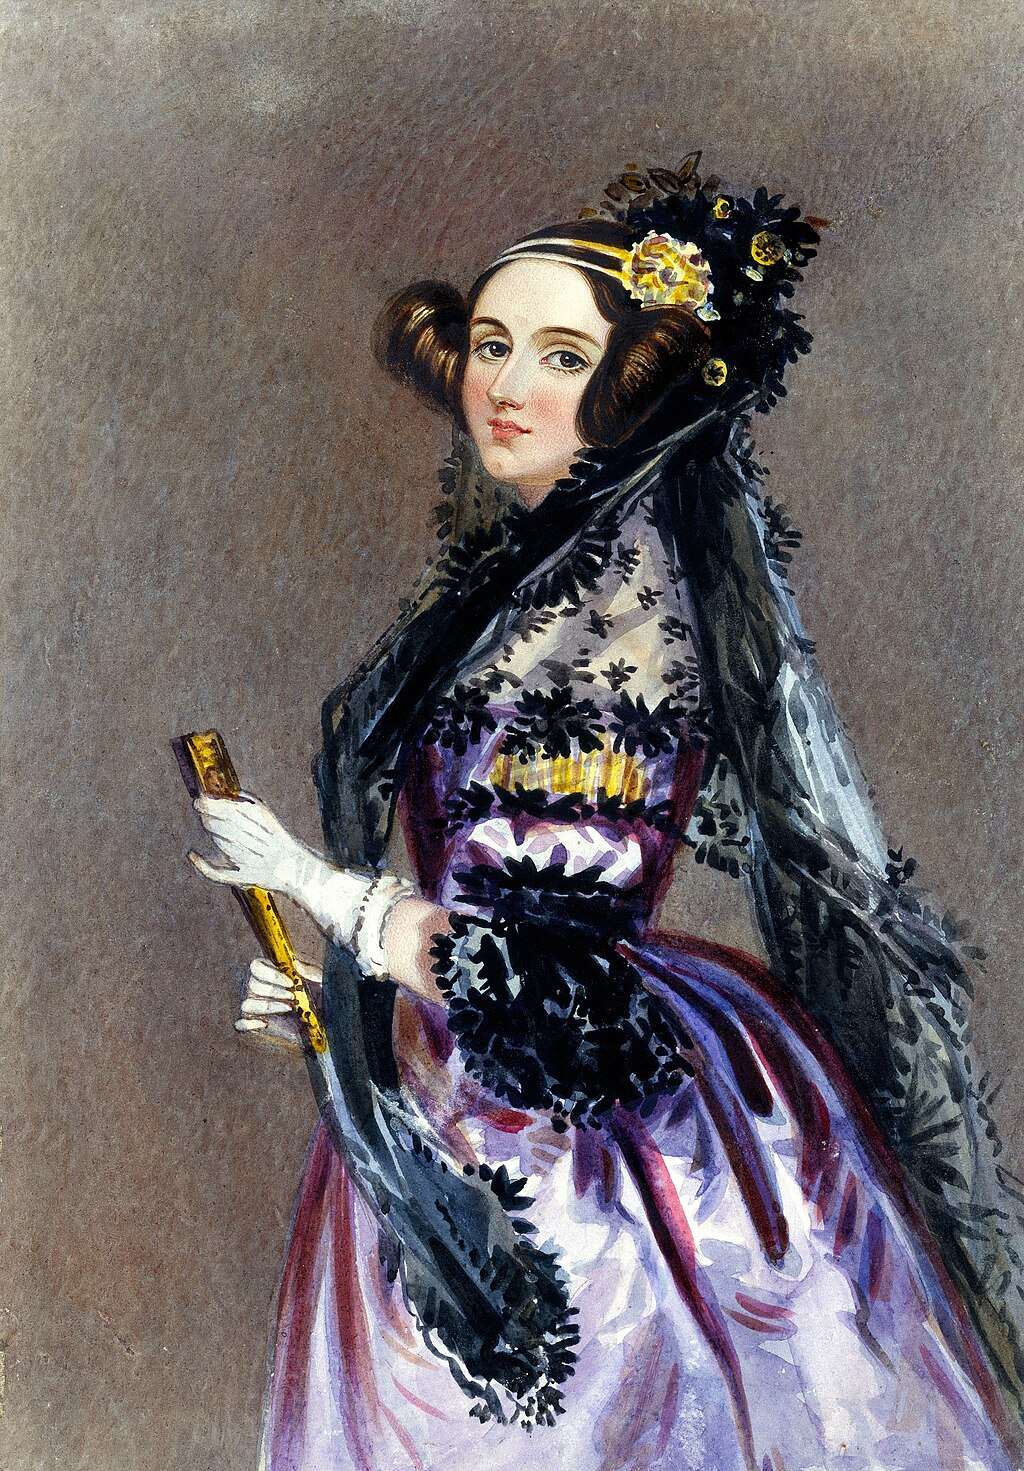
\includegraphics[width=0.3\textwidth]{images/Ada_Lovelace_portrait.jpg}
            \caption{Ada Lovelace 肖像}
        \end{figure}
\end{frame}

\begin{frame}[t]{1843: Ada Lovelace - 第一位程序员}
        \begin{itemize}
            \item 与 Charles Babbage（查尔斯·巴贝奇）合作研究其 \textbf{分析机 (Analytical Engine)}
            \item 《Lovelace 与 Babbage 的惊险冒险》（漫画）
        \end{itemize}

        \begin{figure}[b]
        \centering
        \subfloat[分析机试验模型]{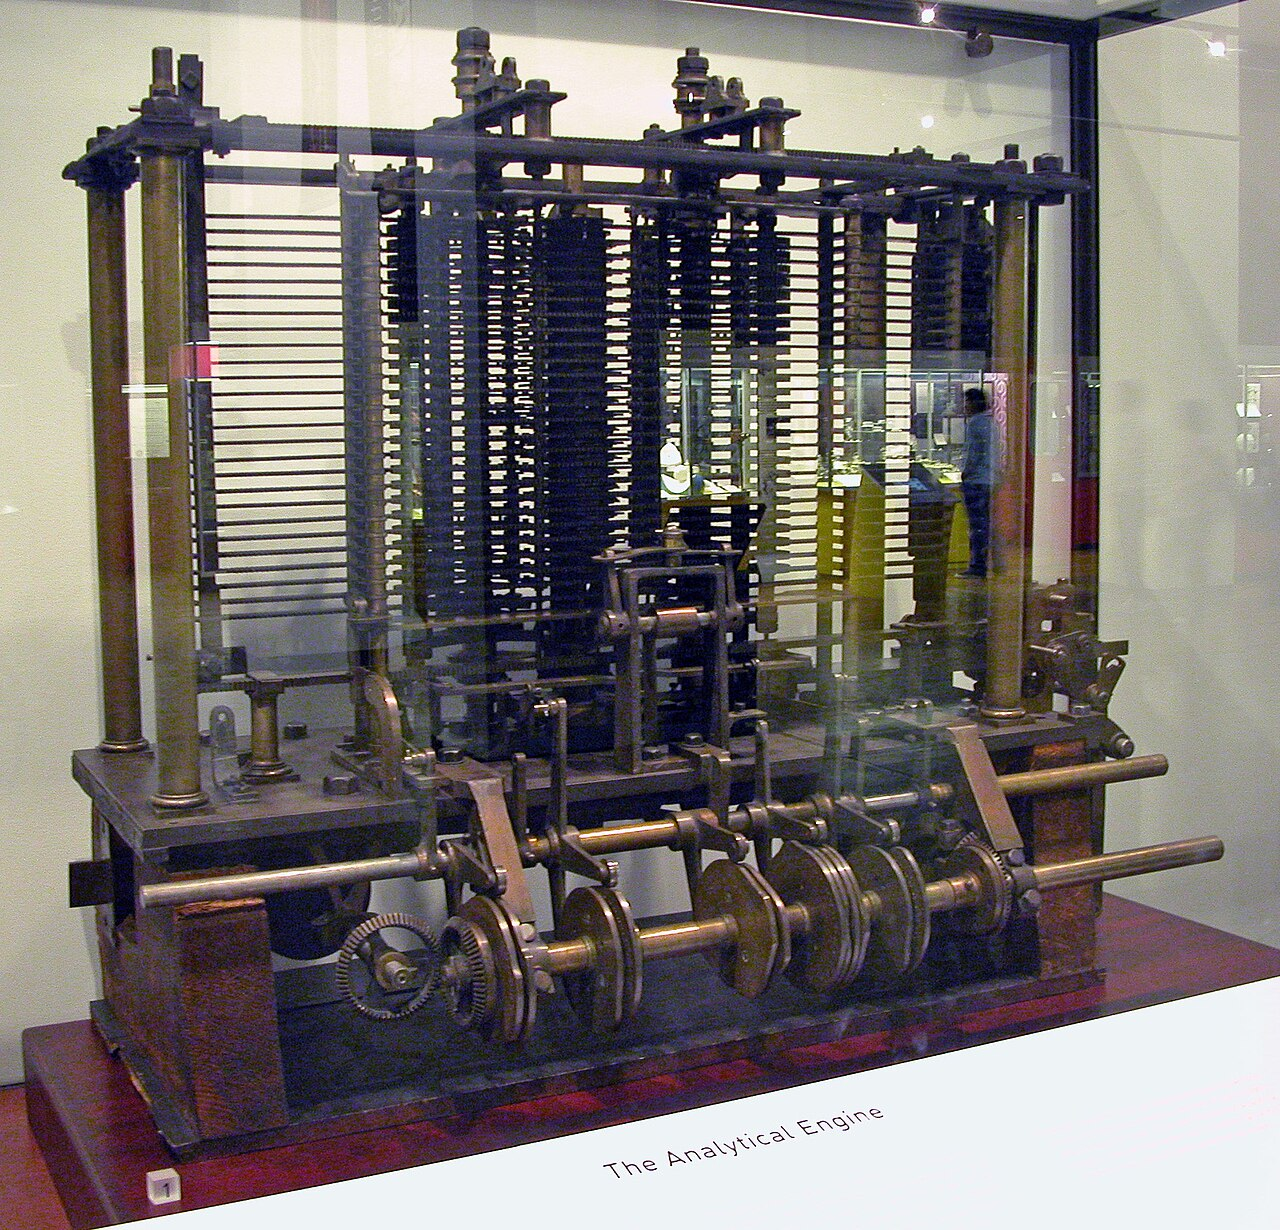
\includegraphics[height=4cm]{images/AnalyticalMachine_Babbage_London.jpg}}\qquad    
        \subfloat[漫画封面]{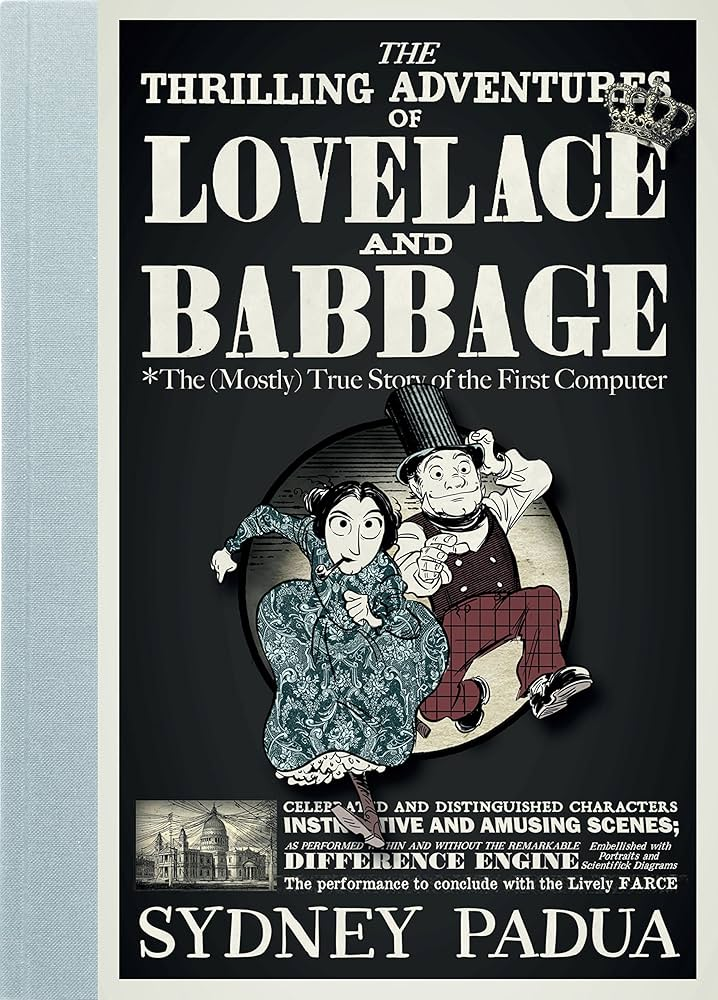
\includegraphics[height=4cm]{images/Comic_cover.jpg}}    
        \caption{分析机}
        \end{figure}
\end{frame}

\begin{frame}[t]{1843: Ada Lovelace - 第一位程序员}
	\begin{figure}
	\begin{center}
		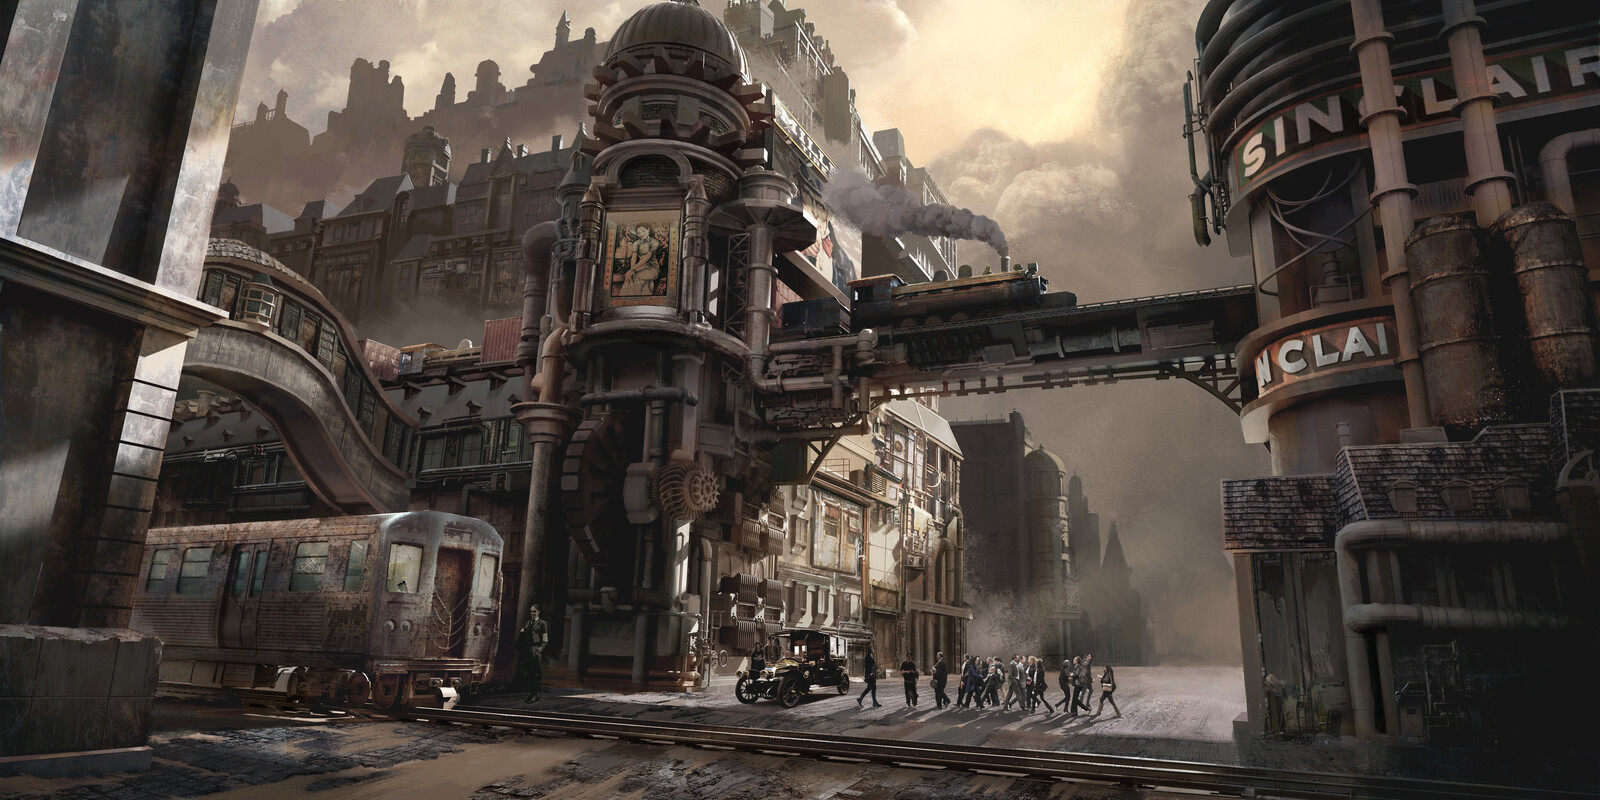
\includegraphics[width=.8\textwidth]{images/steampunk.jpg}
	\end{center}
	\caption{蒸汽朋克}
	\end{figure}
\end{frame}

\begin{frame}[t]{1843: Ada Lovelace - 第一位程序员}
        \begin{itemize}
            \item 她翻译了一篇关于分析机的意大利文章，并添加了大量的个人\textbf{注释 (Notes)}
            \item \textbf{Note G} 包含了被认为是世界上第一个计算机程序的内容
        \end{itemize}
        \begin{figure}[b]
            \centering
            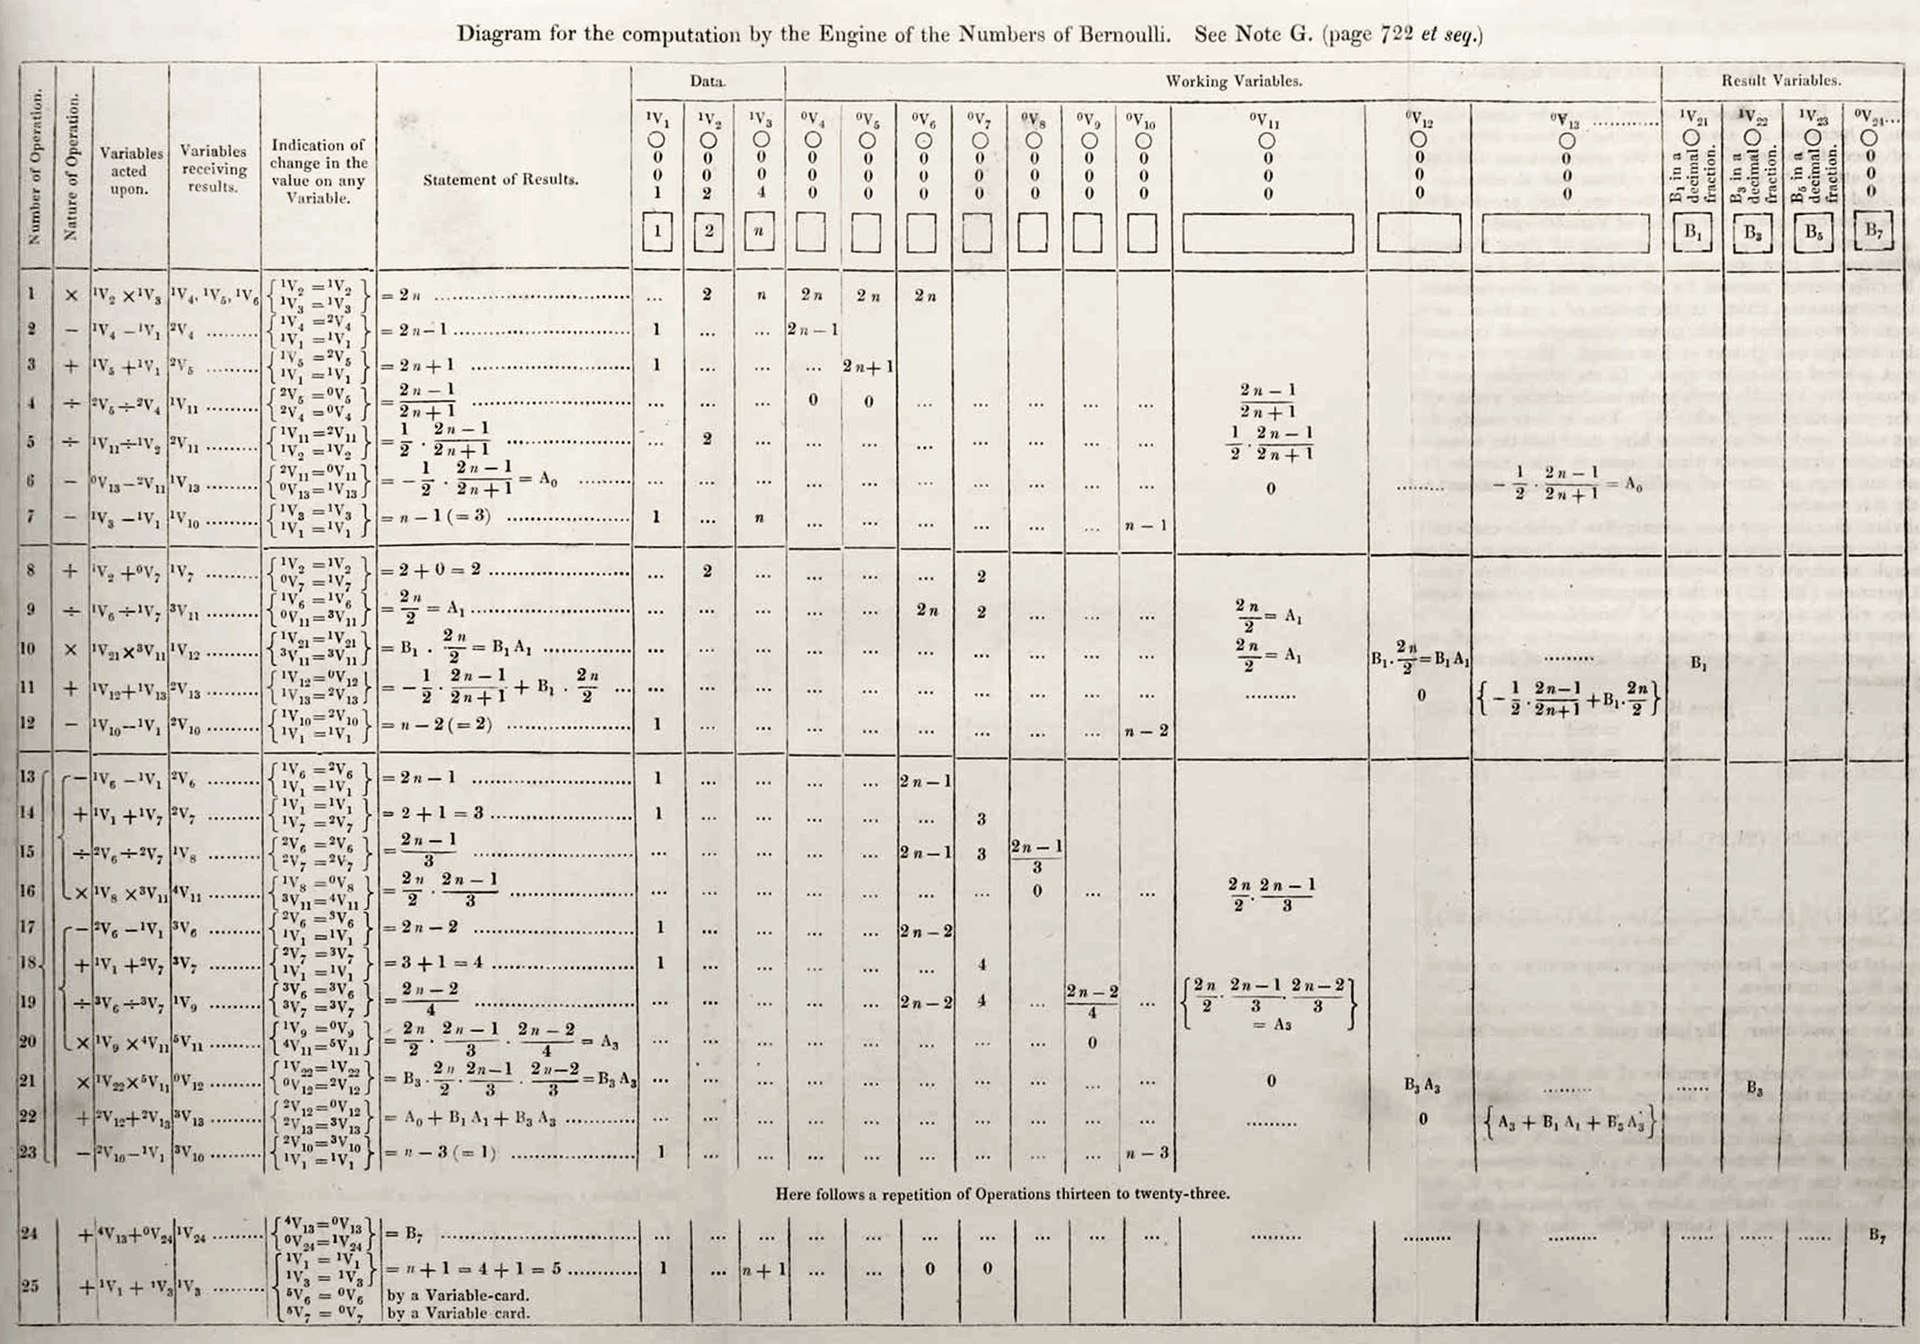
\includegraphics[width=0.5\textwidth]{images/Diagram_for_the_computation_of_Bernoulli_numbers.jpg}
            \caption{第一个程序}
        \end{figure}
\end{frame}

\begin{frame}[t]{Lovelace 的遗产}
\begin{itemize}
    \item \textbf{Ada 编程语言}：1980年由美国国防部以她的名字命名。设计用于大规模、安全关键型系统。
    \item \textbf{Ada Lovelace 日}：每年十月的第二个星期二举行的国际性庆祝活动。
\end{itemize}

    \begin{figure}[b]
        \centering
        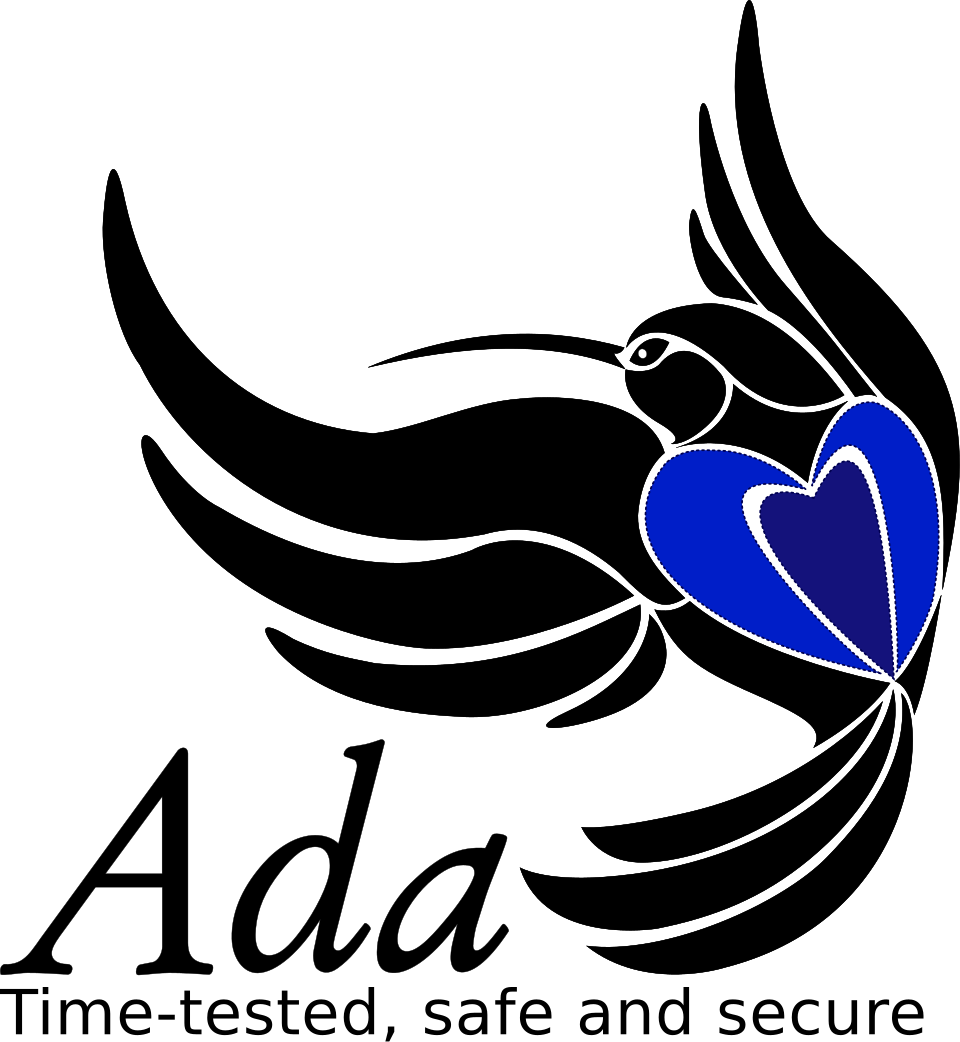
\includegraphics[width=0.3\textwidth]{images/Ada_logo.png}
        \caption{Ada 编程语言吉祥物}
    \end{figure}
\end{frame}

\begin{frame}[t]{从愿景到现实}
\begin{center}
    \begin{tabular}{c}
        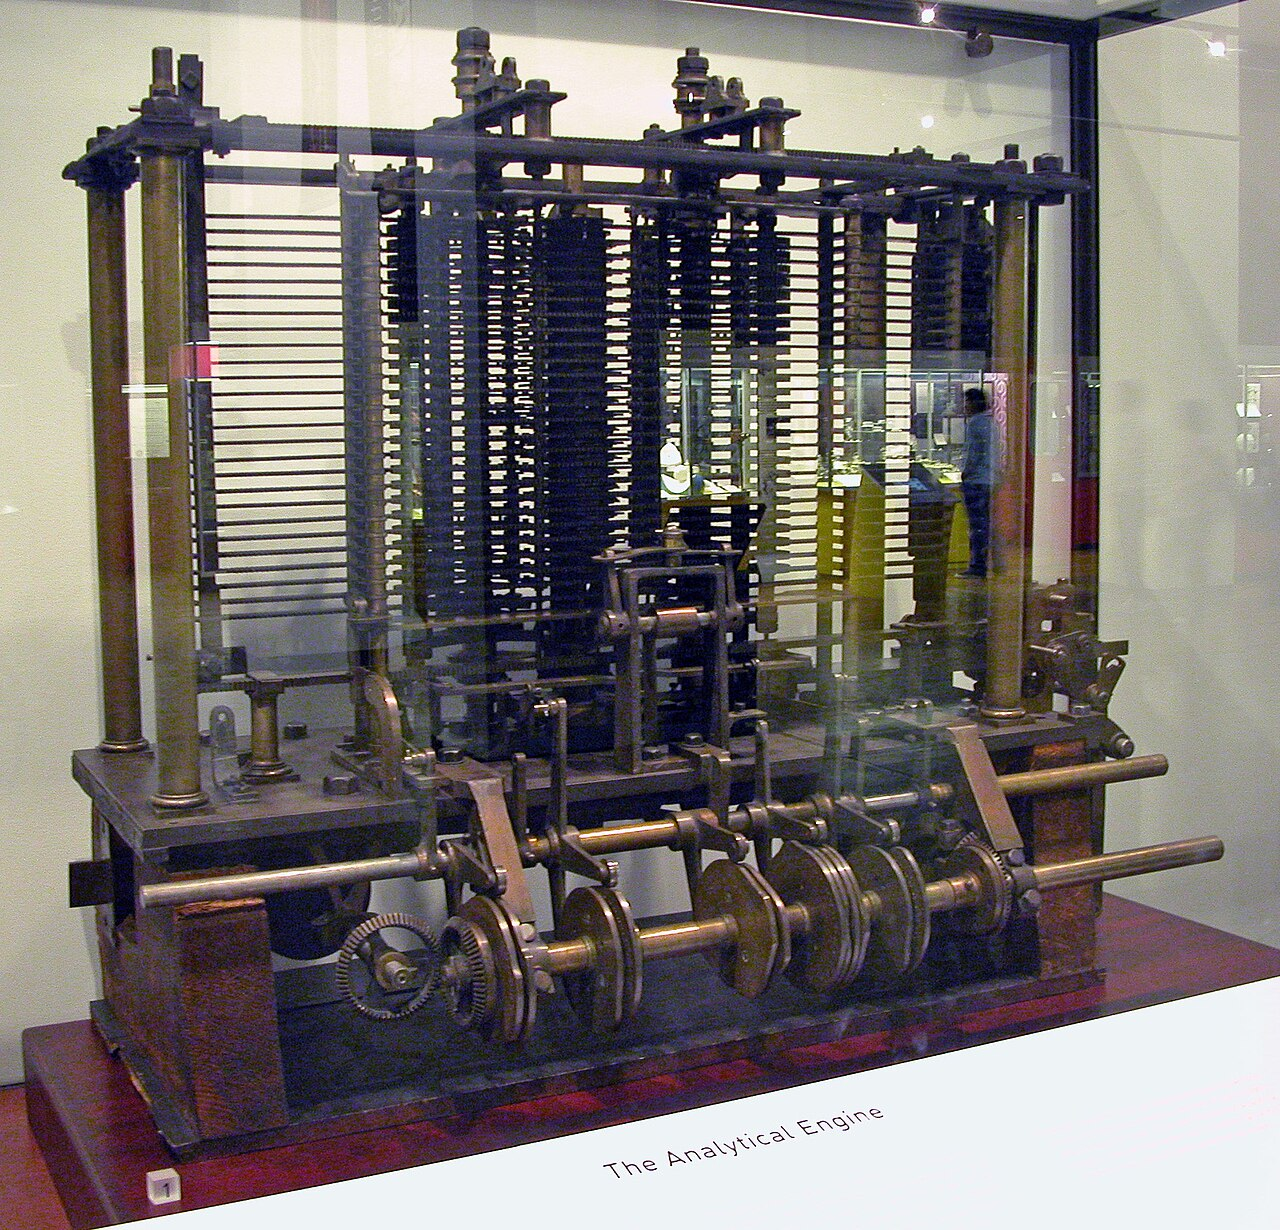
\includegraphics[width=0.25\textwidth]{images/AnalyticalMachine_Babbage_London.jpg} \\
        \textbf{1840s} Lovelace 的理论程序 \\
        $\Downarrow$ \textbf{~100 年} $\Downarrow$ \\
        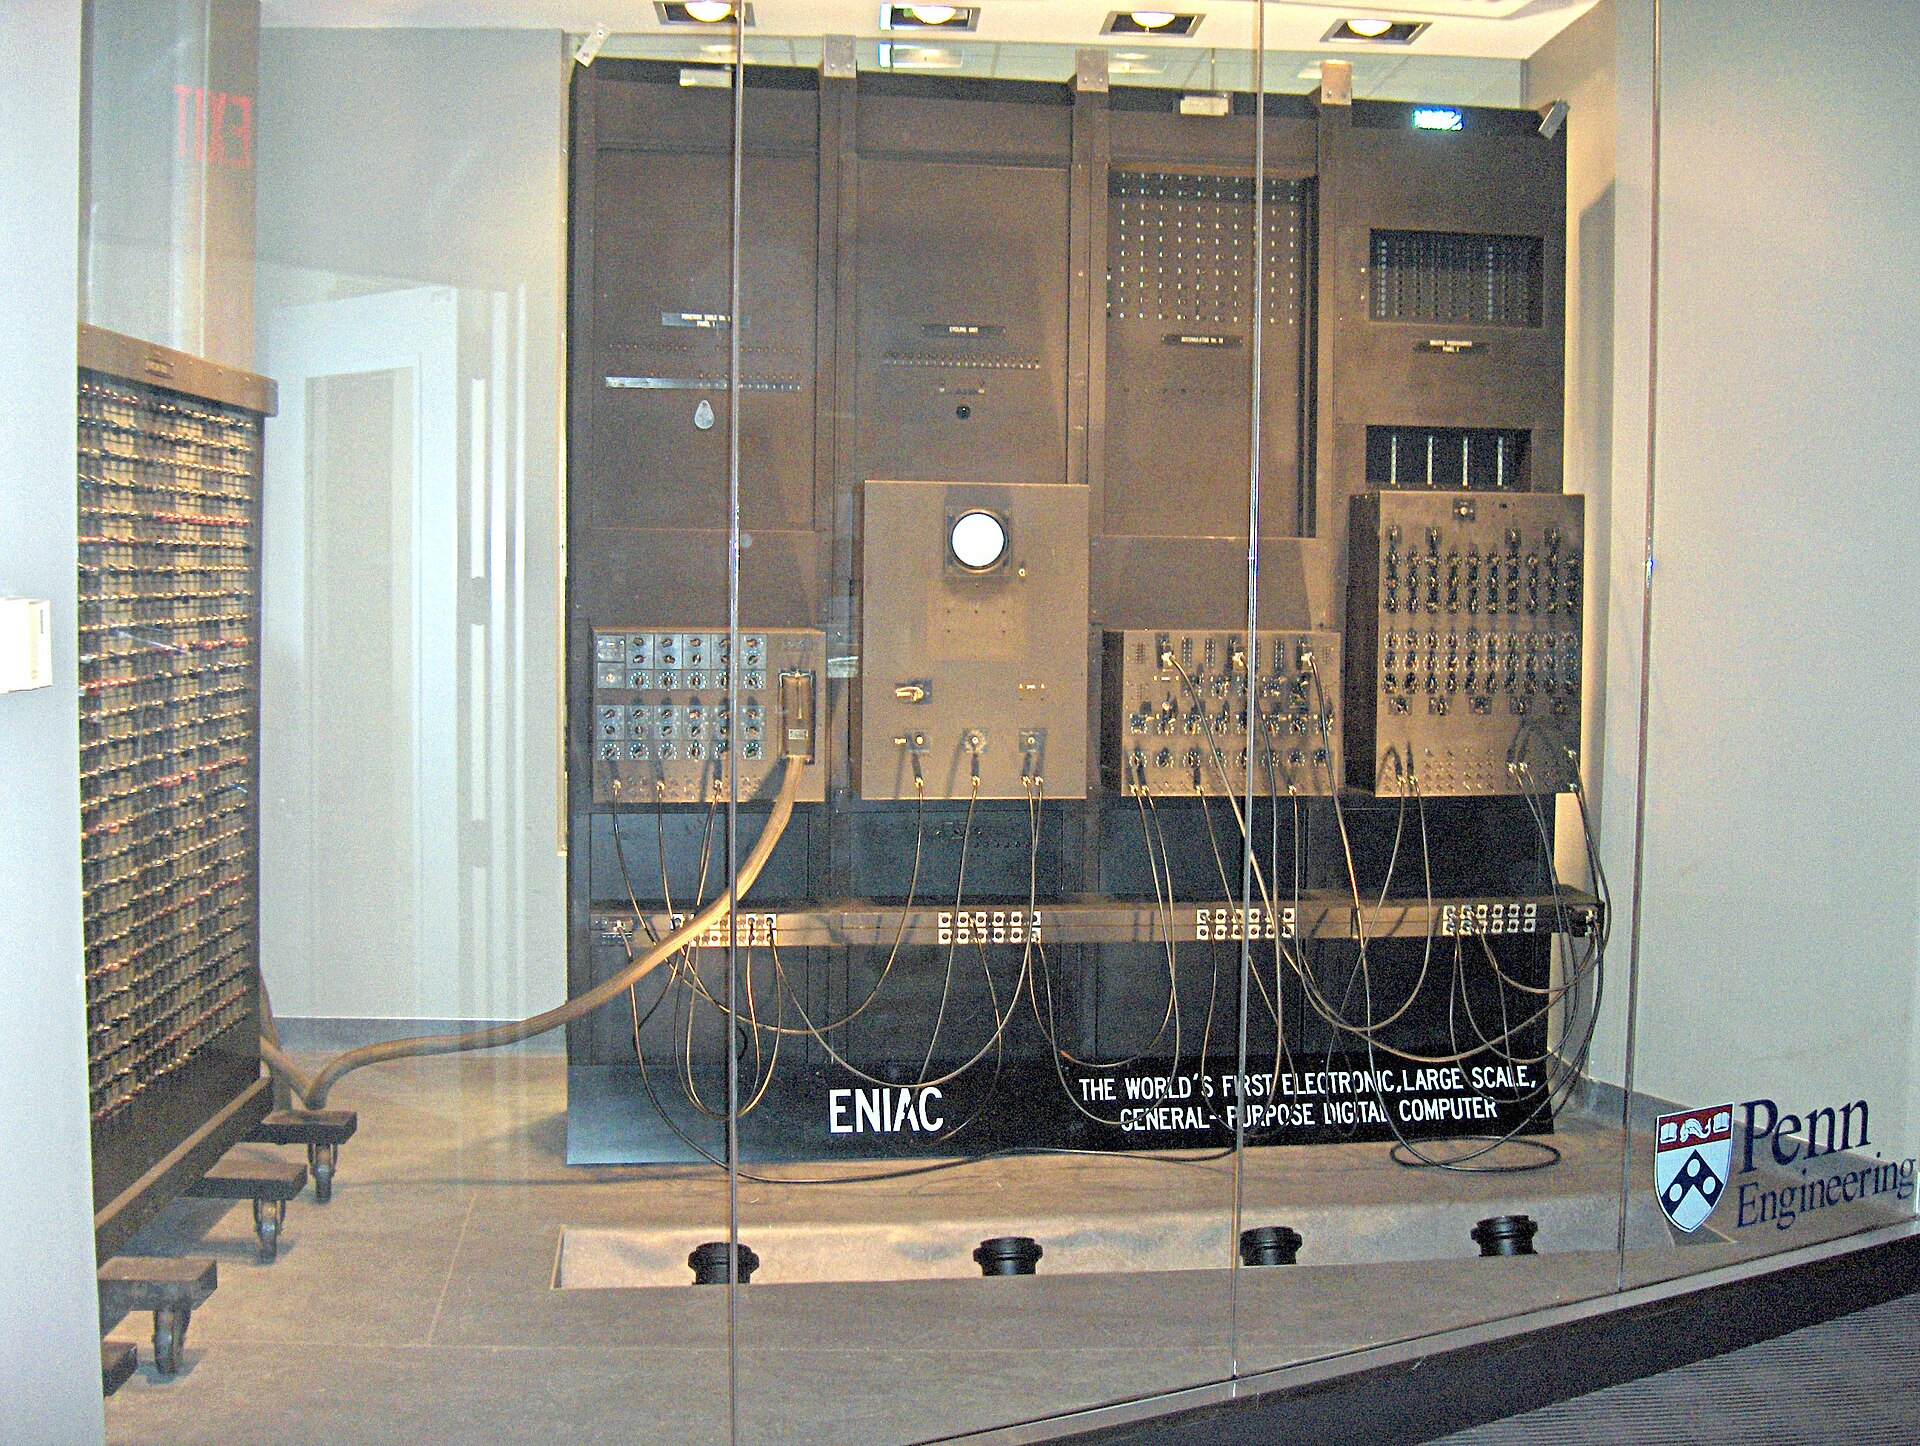
\includegraphics[width=0.25\textwidth]{images/ENIAC_Penn1.jpg} \\
        \textbf{1940s} ENIAC - 第一台电子计算机 \\
    \end{tabular}
\end{center}
\end{frame}

\begin{frame}[t]
\frametitle{高级语言的黎明}
\begin{itemize}
    \item \textbf{1950s 背景}：使用机器码/汇编进行编程既繁琐又容易出错
    \item \textbf{愿景}：创建更易于人类阅读且与机器无关的语言
    \item \textbf{出现的两条路径}：
    \begin{itemize}
        \item \textbf{Fortran (1957)}：为科学计算设计 - \textit{命令式}
        \item \textbf{Lisp (1958)}：为人工智能研究设计 - \textit{函数式}
    \end{itemize}
\end{itemize}

\begin{center}
    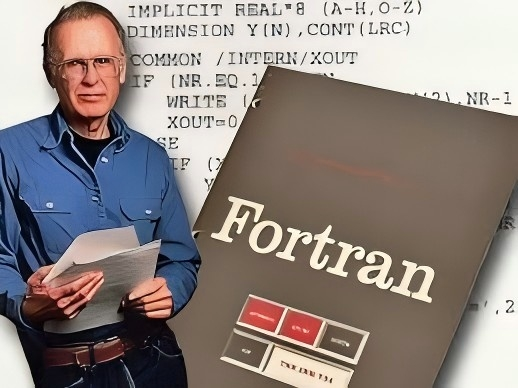
\includegraphics[width=0.3\textwidth]{images/fortran.jpg}
    \quad
    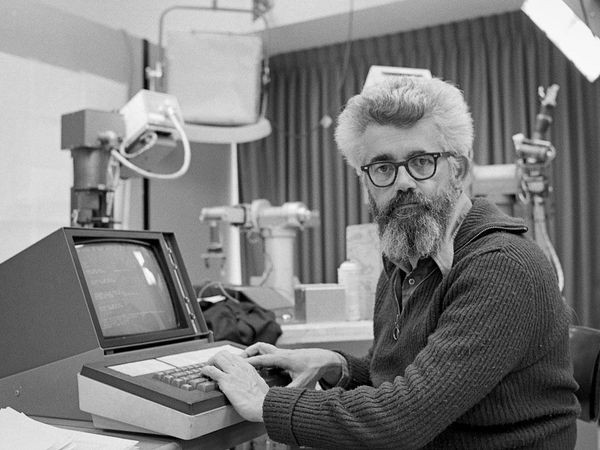
\includegraphics[width=0.3\textwidth]{images/lisp.jpg}
    \\\scriptsize{左：John Backus, Fortran 创始人；右：John McCarthy, Lisp 创始人}
\end{center}
\end{frame}

\begin{frame}[t]
\frametitle{Fortran：第一门高级语言}
\begin{itemize}
    \item \textbf{名称}：公式翻译系统 (FORmula TRANslating system)
    \item \textbf{创建者}：1957年由 IBM 的 John Backus 创建
    \item \textbf{主要目标}：使科学计算更简单、更高效
    \item \textbf{关键创新}：
    \begin{itemize}
        \item 历史上第一个编译器
        \item 类似于代数的数学符号
        \item 数组操作和复数处理
        \item 令人惊讶的高效代码生成
    \end{itemize}
    \item \textbf{影响}：彻底改变了科学和工程计算
\end{itemize}
\end{frame}

\begin{frame}[fragile,t]
\frametitle{Fortran Code Example}
\scriptsize
\begin{lstlisting}[language=Fortran, caption=Fortran 77 Style]
C AREA OF A TRIANGLE WITH HERON'S FORMULA
      PROGRAM TRIANGLE
      REAL A, B, C, AREA, S
      
      READ *, A, B, C
      S = (A + B + C) / 2.0
      AREA = SQRT(S * (S - A) * (S - B) * (S - C))
      
      PRINT *, 'AREA = ', AREA
      END PROGRAM
\end{lstlisting}

\begin{itemize}
    \item \textbf{命令式风格}：显式的操作序列
    \item \textbf{数学焦点}：公式的直接翻译
    \item \textbf{简单数据流}：变量被原地修改
    \item \textbf{固定格式}：早期版本要求特定的列位置
\end{itemize}
\end{frame}

\begin{frame}[t]
\frametitle{Lisp：第二门高级语言}
\begin{itemize}
    \item \textbf{名称}：列表处理 (LISt Processing)
    \item \textbf{创建者}：1958年由 MIT 的 John McCarthy 创建
    \item \textbf{主要目标}：人工智能研究
    \item \textbf{关键创新}：
    \begin{itemize}
        \item 函数式编程范式
        \item 链表作为基本数据结构
        \item 垃圾回收机制
        \item 同质性 (Homoiconicity)：代码即数据，数据即代码
        \item 递归作为主要控制结构
    \end{itemize}
    \item \textbf{影响}：人工智能研究和函数式编程的基础
\end{itemize}
\end{frame}

\begin{frame}[fragile,t]
\frametitle{Lisp 代码示例}
\scriptsize
\begin{lstlisting}[language=Lisp, caption=Common Lisp Style]
;; 使用递归计算阶乘
(defun factorial (n)
  (if (<= n 1)
      1
      (* n (factorial (- n 1)))))

;; 在列表上映射函数
(defun square-list (numbers)
  (mapcar #'(lambda (x) (* x x)) numbers))

;; 使用高阶函数
(let ((numbers '(1 2 3 4 5)))
  (print (factorial 5))
  (print (square-list numbers)))
\end{lstlisting}

\begin{itemize}
    \item \textbf{函数式风格}：强调表达式而非语句
    \item \textbf{递归思维}：通过递归分解问题
    \item \textbf{列表操作}：内置的列表处理操作
\end{itemize}
\end{frame}

\begin{frame}[t]
\frametitle{范式对比：命令式 vs 函数式}
\begin{itemize}
    \item \textbf{Fortran (命令式范式)}:
    \begin{itemize}
        \item \textit{哲学}：“如何计算” - 步骤序列
        \item \textit{状态变化}：变量被修改
        \item \textit{控制结构}：循环、条件判断、goto
        \item \textit{主要抽象}：过程和子程序
        \item \textit{内存管理}：手动/基于栈
    \end{itemize}
    
    \item \textbf{Lisp (函数式范式)}:
    \begin{itemize}
        \item \textit{哲学}：“计算什么” - 表达式与变换
        \item \textit{不可变性}：尽可能避免改变状态
        \item \textit{控制结构}：递归、函数组合
        \item \textit{主要抽象}：函数作为一等公民
        \item \textit{内存管理}：自动垃圾回收
    \end{itemize}
\end{itemize}
\end{frame}

\begin{frame}[t]
\frametitle{设计哲学对比}
\begin{itemize}
    \item \textbf{Fortran 的实用导向}:
    \begin{itemize}
        \item 专为数值计算效率而设计
        \item 紧密映射数学符号
        \item 针对数组操作和线性代数进行了优化
        \item 最小化语法，最大化计算能力
        \item 目标用户：科学家和工程师
    \end{itemize}
    
    \item \textbf{Lisp 的理论基础}:
    \begin{itemize}
        \item 基于 Lambda 演算和递归函数理论
        \item 拥抱符号计算和人工智能问题
        \item 通过宏 (Macros) 实现强大的元编程
        \item 通过 REPL 环境进行交互式开发
        \item 目标用户：AI 研究员和计算机科学家
    \end{itemize}
\end{itemize}
\end{frame}

\subsection{起源}

\begin{frame}[t]{软件工程的黎明}
\begin{itemize}
    \item \textbf{1968 NATO 会议}：“软件工程”一词正式提出
    \item 解决“软件危机” - 软件开发日益增长的复杂性和成本
    \item 核心目标：将工程原则应用于软件开发
\end{itemize}
    \begin{figure}[b]
        \centering
        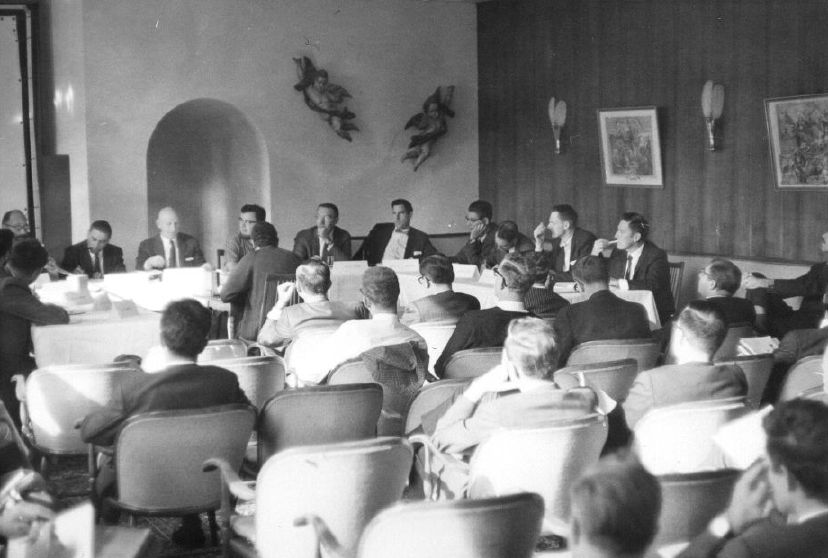
\includegraphics[width=0.3\textwidth]{images/NATO-conference-photo.png}
        \caption{1968 NATO 加米施会议}
    \end{figure}
\end{frame}

\subsection{基础概念}

\begin{frame}[t]{1968: “Goto 语句被认为有害”}
\begin{itemize}
    \item \textbf{Edsger Dijkstra 的开创性信函} (1968)
    \item 主张反对使用 GOTO 语句
    \item 推动结构化编程原则
    \item 现代控制结构（if-else, while, for）的基础
    \item 强调代码的可读性和可维护性
\end{itemize}
\begin{block}{Dijkstra 的洞察}
程序测试可以用来展示 Bug 的存在，但永远无法展示它们的缺失。
\end{block}
\end{frame}

\begin{frame}[t]{Dijkstra 论自然语言编程 (1978)}
\begin{itemize}
    \item Dijkstra 强烈反对“用自然语言告诉计算机做什么”的设想。
    \begin{itemize}
        \item 自然语言具有高度的\textbf{模糊性 (Ambiguity)}。
        \item 编程的本质是\textbf{严谨的思维过程}。如果一个人能够清晰严谨地用自然语言描述问题，他其实已经在编写一种形式化语言。
    \end{itemize}
\end{itemize}
\begin{quote}
    “所谓自然语言的‘自然性’，归根结底，不过是我们能轻松地用它说出那些荒谬性并不显而易见的话。” —— E.W. Dijkstra
\end{quote}
\end{frame}

\begin{frame}[t]{Dijkstra 论自然语言编程 (1978)}
\begin{figure}
    \centering
    
\includegraphics[width=0.6\textwidth]{images/code.png}
    \caption{那就是代码}
\end{figure}
\end{frame}

% \begin{frame}[t]{LLM 时代的自然语言接口}
% \begin{block}{Prompt Engineering：Dijkstra 错了吗？}
% \begin{itemize}
%     \item \textbf{范式转移}：LLM 证明了模糊的自然语言可以被转化为精确的代码。
%     \item \textbf{验证的必要性}：虽然输入是自然的，但输出（代码）必须经过编译器和测试集的验证。
%     \item \textbf{混合模式}：未来的编程可能不是“纯自然语言”，而是以自然语言驱动、以形式化逻辑（如类型系统）为约束的“意图编程”。
% \end{itemize}
% \end{block}
% \end{frame}

\begin{frame}{当代回响}
\begin{itemize}
    \item 2026年，LLM让“自然语言编程”成为现实：Karpathy几乎不再亲手写码，Stripe每周合并1300个Agent PR
    \item 但AI编程实践的教训与Dijkstra的警告惊人地吻合：
\end{itemize}
\vspace{0.2cm}
\begin{enumerate}
    \item 甜蜜期：动动嘴就能跑出Demo → 接受“不用想太清楚就能开始”
    \item 阵痛期：AI习惯性“漏需求”，架构松散，上下文一长就“降智”
    \item 回归期：最有效的流程变成了：描述意图 $\rightarrow$ 转化为Spec $\rightarrow$ AI分析排除矛盾 $\rightarrow$ 人类审查 $\rightarrow$ 测试套件 $\rightarrow$ 分拆执行
\end{enumerate}
\vspace{0.2cm}
\small 这个流程的每一步，本质上都是在把自然语言的“毛坯”，精加工成形式化的“构件”。
\end{frame}

\begin{frame}[t]{1975: 人月神话}
\begin{columns}
    \begin{column}{0.6\textwidth}
        \begin{itemize}
            \item \textbf{Frederick Brooks 的经典著作} (1975)
            \item 基于管理 IBM OS/360 开发的经验
            \item \textbf{核心论点}：“向进度落后的软件项目添加人力会使其更慢”
            \item \alert{布鲁克斯法则}：由于沟通成本，在软件工作中“人月”是一个危险且错误的度量单位。
            \item “没有银弹”
        \end{itemize}
    \end{column}
    \begin{column}{0.4\textwidth}
        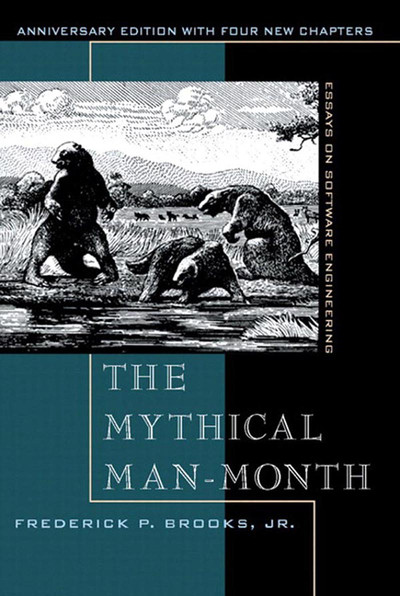
\includegraphics[width=0.6\textwidth]{images/Mythical Man-Month.jpg}
    \end{column}
\end{columns}
\end{frame}

\begin{frame}[t]{1986: 没有银弹 (No Silver Bullet)}
\begin{itemize}
    \item \textbf{Fred Brooks 的核心观点}：在十年内，没有任何单一的技术或管理进展能让软件生产率提高一个数量级。
    \item \textbf{两种复杂度}：
    \begin{itemize}
        \item \alert{本质复杂度 (Essential Complexity)}：软件所要解决的业务逻辑、数据关系和算法本身的复杂性。
        \item \alert{附属性复杂度 (Accidental Complexity)}：由于开发环境、语言语法、陈旧工具等引起的非必要困难。
    \end{itemize}
    \item \textbf{结论}：大多数现代进步（如高级语言、IDE）只解决了附属性复杂度。本质复杂度无法通过“魔法”消除。
\end{itemize}
\begin{figure}
    \centering
    
\includegraphics[width=0.4\textwidth]{images/silver_bullet.jpg}
    \caption{软件工程中没有万灵药}
\end{figure}
\end{frame}

\begin{frame}[t]{LLM 时代的“银弹”讨论}
\begin{block}{LLM 是终极银弹吗？}
\begin{itemize}
    \item \textbf{附属性复杂度的终结}：LLM 极大地消除了语法记忆、API 查找和样板代码编写的负担（接近零附属性复杂度）。
    \item \textbf{本质复杂度的回归}：即使代码生成速度快了 10 倍，\textbf{需求定义、系统架构设计和逻辑正确性}（本质复杂度）依然由人类承担。
    \item \textbf{新挑战}：AI 幻觉引入了新的测试和验证成本。
\end{itemize}
\end{block}
\end{frame}

\begin{frame}[t]{观点演变总结}
\begin{table}
\scriptsize
\centering
\begin{tabular}{|l|p{4cm}|p{4cm}|}
\hline
\textbf{核心议题} & \textbf{经典观点 (Brooks/Dijkstra)} & \textbf{LLM 时代特点} \\ \hline
\textbf{生产力瓶颈} & 本质复杂度（逻辑、沟通）不可逾越。 & LLM 加速了实现过程，但沟通和逻辑确认仍是瓶颈。 \\ \hline
\textbf{编程媒介} & 必须使用严谨的数学/形式化语言。 & 自然语言成为第一接口，但代码仍作为底层“真理”。 \\ \hline
\textbf{程序员角色} & 逻辑构建者与细节实现者。 & \textbf{审查者 (Reviewer)} 与 \textbf{需求策展人 (Curator)}。 \\ \hline
\end{tabular}
\caption{经典理论在 AI 时代的延续与转变}
\end{table}
\end{frame}

\begin{frame}[t]{编程之道}
\begin{columns}
    \begin{column}{0.6\textwidth}
        \scriptsize
        \begin{itemize}
            \item 一位经理找到大师级程序员，向他展示了一个新应用的需求文档。经理问大师：“如果我分配五个程序员来设计这个系统，需要多长时间？”
            \item “需要一年，”大师不假思索地答道。
            \item “但是我们现在就需要这个系统，甚至越快越好！如果我分配十个程序员，需要多长时间？”
            \item 大师级程序员皱了皱眉头。
            \item “那样的话，需要两年。”
            \item “那如果我分配一百个程序员呢？”
            \item 大师级程序员耸了耸肩。
            \item “那么设计将永远无法完成，”他说。
        \end{itemize}
    \end{column}
    \begin{column}{0.4\textwidth}
        \begin{figure}
            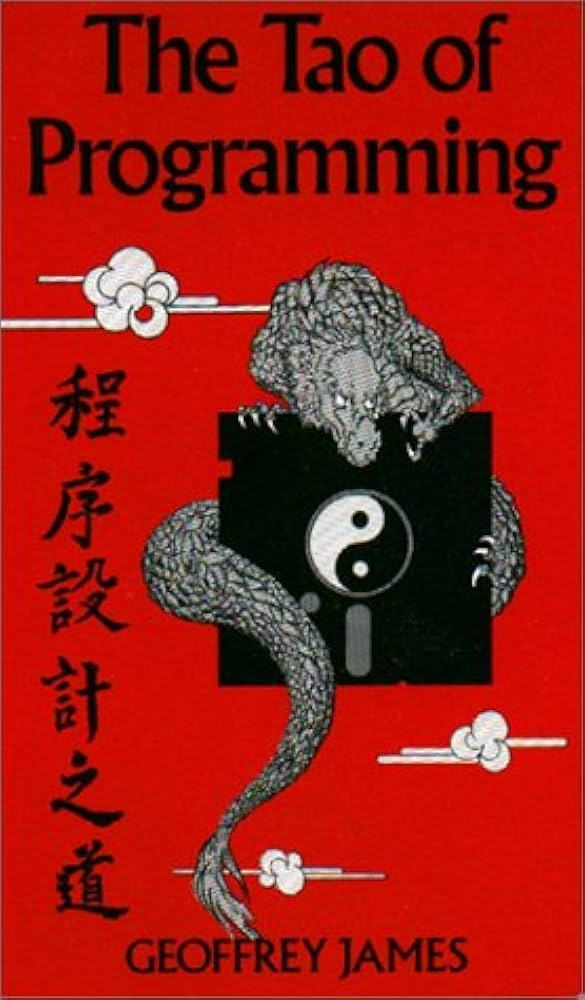
\includegraphics[width=0.6\textwidth]{images/tao.jpg}
        \end{figure}
    \end{column}
\end{columns}
\end{frame}

\begin{frame}[t]{编程之道}
    \scriptsize
    \begin{itemize}
        \item 道生机器语言，机器语言生汇编语言。
        \item 汇编语言生编译器。至今已有万种语言。
        \item 每种语言各有所用，无论多么卑微。
        \item 每种语言都表达了软件的阴阳。每种语言在道中皆有其位。
        \item 但如果可以避免，请不要用 COBOL 编程。
    \end{itemize}
    \begin{block}{道德经}
        \begin{itemize}
            \item 道生一，一生二，二生三，三生万物。
            \item The Tao gave birth to One, One gave birth to Two, Two gave birth to Three, Three gave birth to ten thousand things.
        \end{itemize}
    \end{block}
    \begin{figure}
        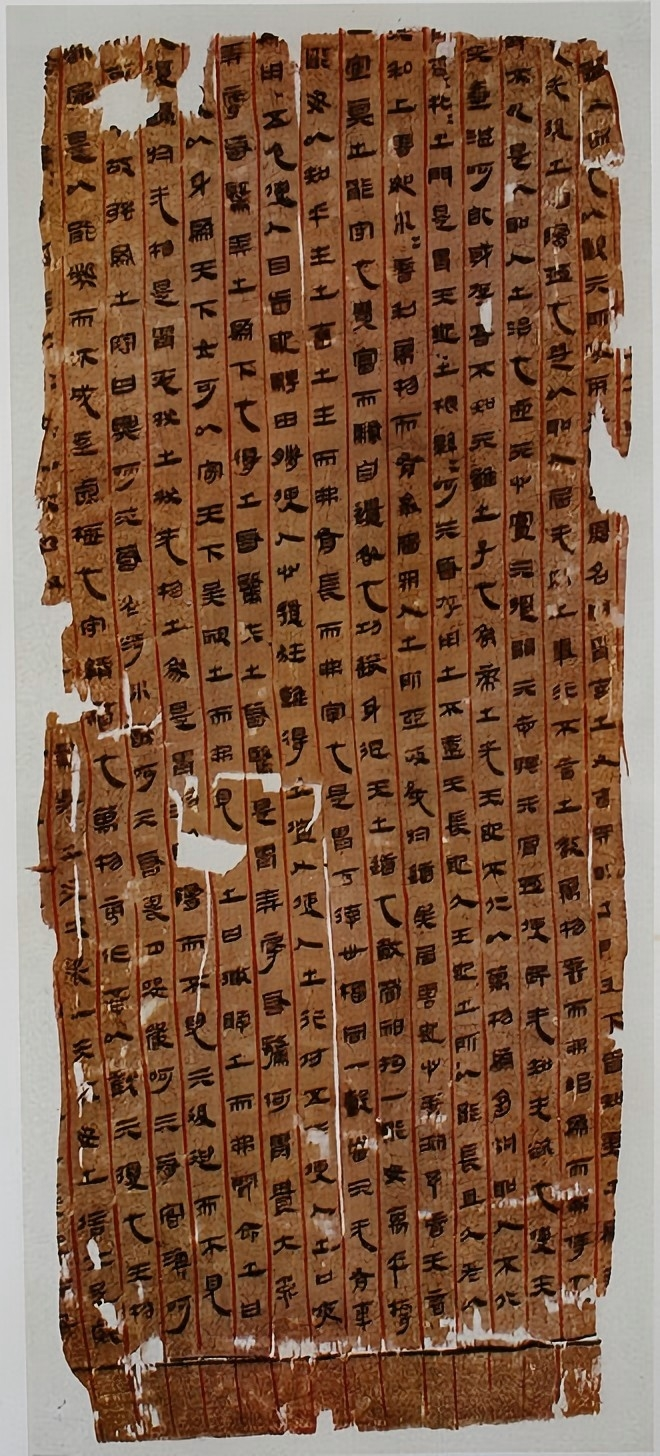
\includegraphics[width=0.1\textwidth]{images/taoist.jpg}
        \caption{《道德经》帛书（公元前2世纪）}
    \end{figure}
\end{frame}

\subsection{关键里程碑}

\begin{frame}[t]{1984: 关于信任信任的反思}
\begin{itemize}
    \item \textbf{Ken Thompson 的图灵奖演讲} (1984)
    \item 编译器可以插入能够自我传播的后门
    \item 软件供应链安全的基础性洞察
\end{itemize}
\begin{figure}
    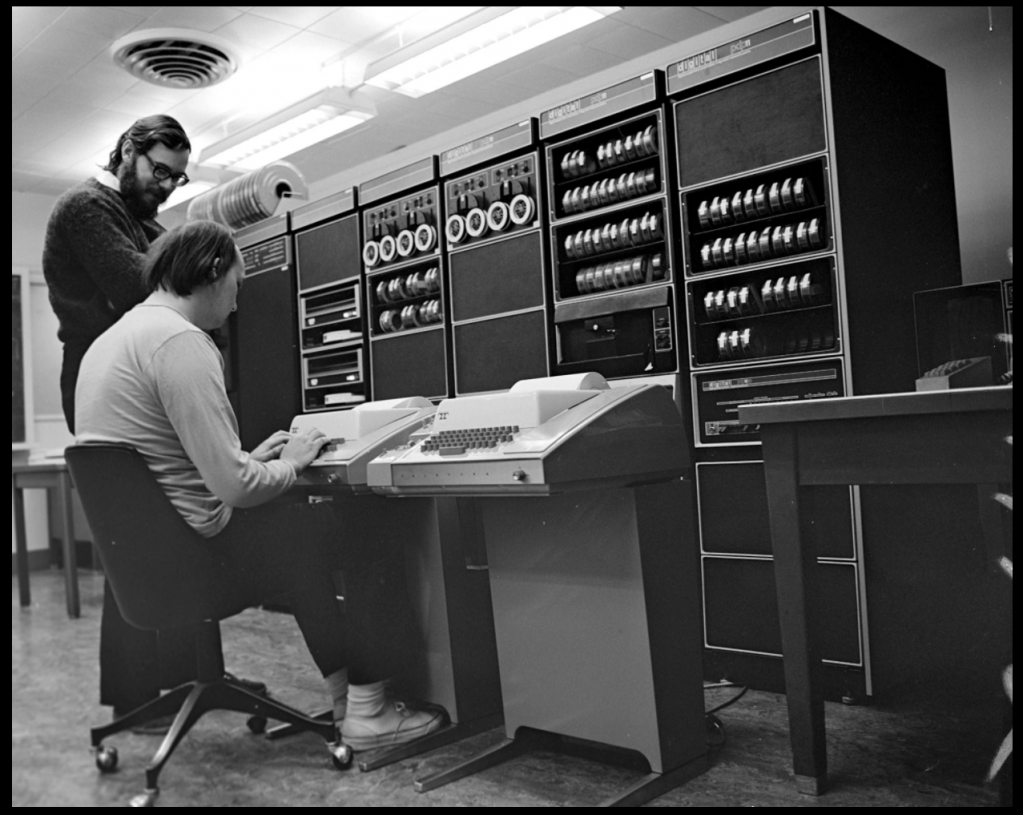
\includegraphics[width=0.3\textwidth]{images/Ken_UNIX.png}
    \caption{Ken Thompson 和 Dennis Ritchie 与 UNIX}
\end{figure}
\pause
\begin{alertblock}{核心启示}
    我们用来构建软件的工具本身必须是可信的。没有终极的信任根。
\end{alertblock}
\end{frame}


\begin{frame}[t]{RogueLike}
    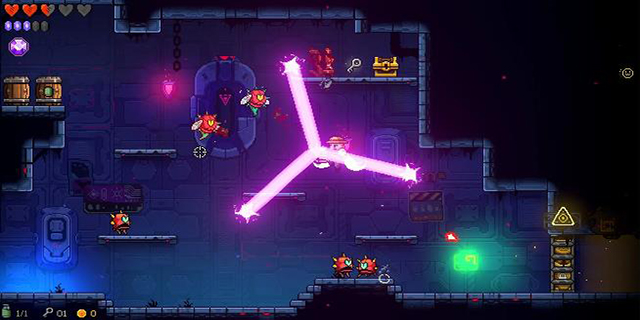
\includegraphics[height=.2\textwidth]{images/roguelike1.jpg} 
    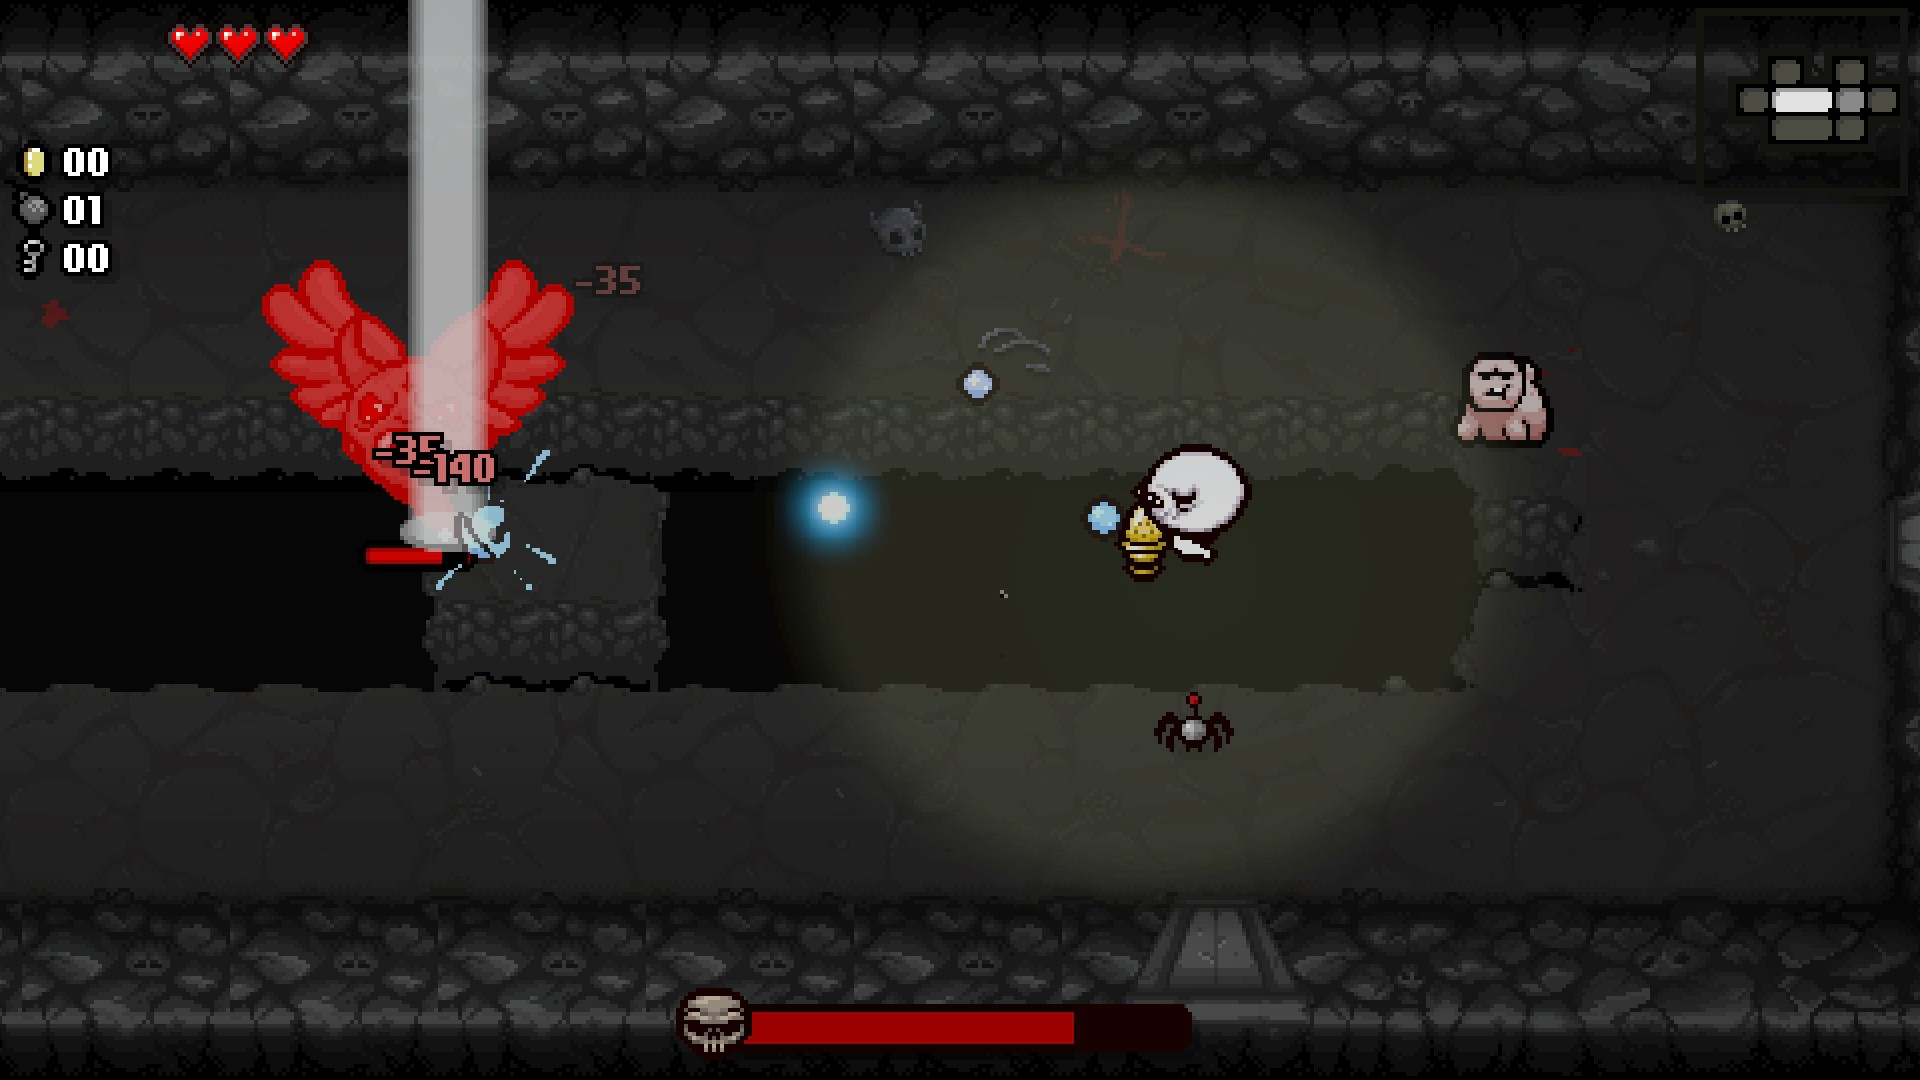
\includegraphics[height=.2\textwidth]{images/roguelike2.jpg} 
\end{frame}
\begin{frame}[t]{Rogue}

    Rogue是迷宫探索式电子游戏，最早由迈克尔·托依和格伦·韦科曼在1980年左右开发\footnote{\url{https://zh.wikipedia.org/wiki/Rogue}}。部分因为游戏内容的过程生成，游戏在1980年代中期大学Unix系统上很流行。Rogue使迷宫探索在电子游戏领域普及，其他开发者制作了诸多统称为“类rogue”（Roguelike）的派生作品。比如它直接给与了Hack灵感，此游戏之后又衍生出NetHack。类rogue还影响了其他类型的商业游戏，如暗黑破坏神
    Rogue在当时的计算机研究者和大学生之间引发轰动，甚至Unix之父之一的肯·汤普逊也沉迷其中。丹尼斯·里奇开玩笑道：“Rogue就是史上最浪费CPU时钟周期的东西（the biggest waste of CPU cycles in history）”
\end{frame}

\begin{frame}[t]{RogueLike}
    游戏玩法核心元素在2008年的柏林国际Roguelike游戏开发大会得到了明确的定义，称之为“柏林准则”
    \begin{itemize}
        \item 通过随机生成地牢来增强可玩性 
        \item 游戏使用永久死亡机制
        \item 游戏是回合制的
        \item 游戏不应该有过多限制
        \item 游戏应该为玩家提供完成同样方式的多种不同方法
        \item 为了生存玩家必须妥善管理自己的资源
        \item 游戏核心内容应是hack and slash
        \item 游戏要求玩家探索地图，寻找宝藏并杜绝背板
    \end{itemize}
\end{frame}

\begin{frame}[t]{Hack and NetHack}
    Hack（1982年）是杰·芬拉森（Jay Fenlason）在肯尼·伍德蓝德（Kenny Woodland）、麦克·托米（Mike Thome）和强纳森·沛恩（Jonathan Payne）的帮助下开发的。他们曾找到Rogue的制作者托伊和阿诺，希望能获取游戏源代码，却遭到拒绝，这迫使他们从原有的游戏草稿设计一个完整的游戏出来。

麦克·史蒂芬森（Mike Stephenson）接手Hack的代码维护工作后，他按照美国宾夕法尼亚大学哲学教授伊兹查克·米勒和电脑极客珍妮特·瓦兹（Janet Walz）的建议改进了这款游戏。这三位组建了一个“开发组”，着手对Hack的源代码做重大修改。部分因为他们的工作主要通过USENET来沟通，他们称修改后的版本为NetHack，Net便是指该游戏通过网络开发。
\end{frame}

\begin{frame}[t]{NetHack}

    \begin{itemize}
        \item NetHack是一款最初在1987年发布的Roguelike单人游戏，拥有由ASCII字符组成的图形界面。它继承了Hack（1985年）及更早的Rogue（1980年）。\footnote{\url{https://zh.wikipedia.org/wiki/NetHack}}
        \item 游戏名字中的“网络”（Net）是指开发过程通过互联网合作完成。
        \item 而“Hack”是指角色扮演游戏的特点——hack and slash。
        \item 玩家扮演一个地下城探险者寻找Yendor的项链。
        \item 玩家需要选择自己所扮演的角色并指定性别、种族、职业和阵营，或者选择让系统随机产生一个角色。游戏者可以扮演经典奇幻角色，比如骑士、野蛮人、巫师、游侠、女武神、僧侣和武士，也可以选择一些比较少见的角色，诸如考古学家、游客和洞穴人。
    \end{itemize}
\end{frame}

\begin{frame}[t]{DnD}
    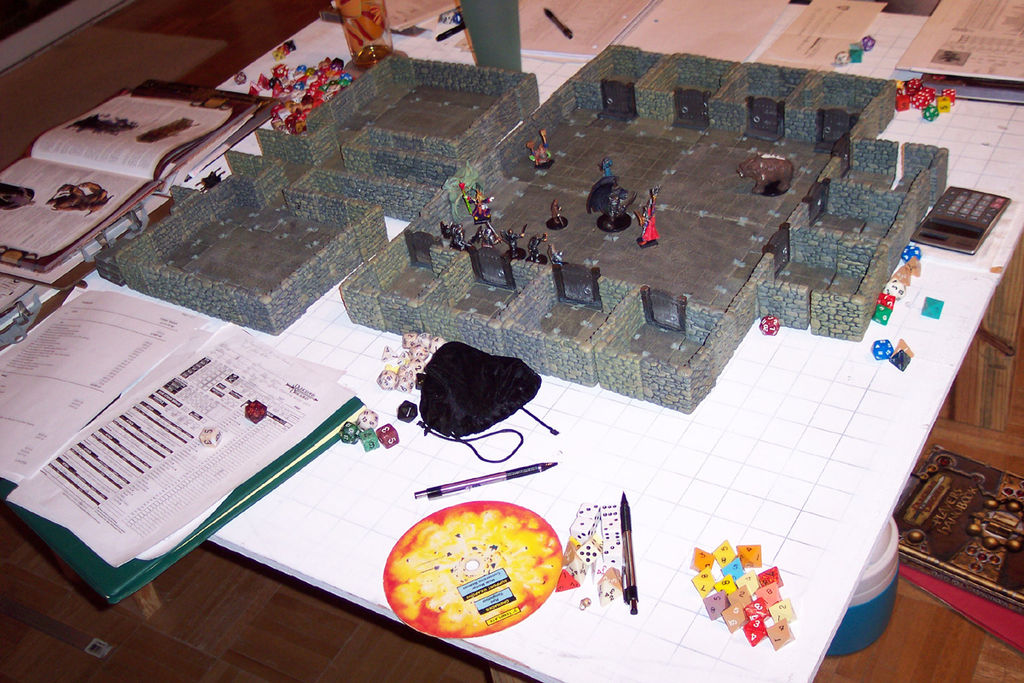
\includegraphics[width=.7\textwidth]{images/dnd.jpg} 
\end{frame}

\begin{frame}[t]{Nethack}
    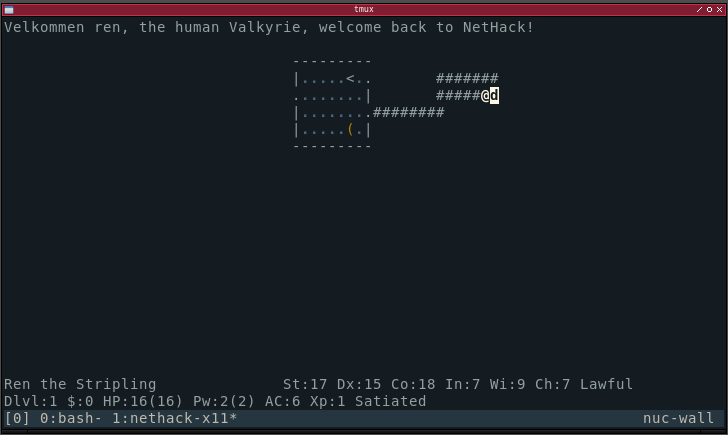
\includegraphics[height=.25\textwidth]{images/nethack.png} 
    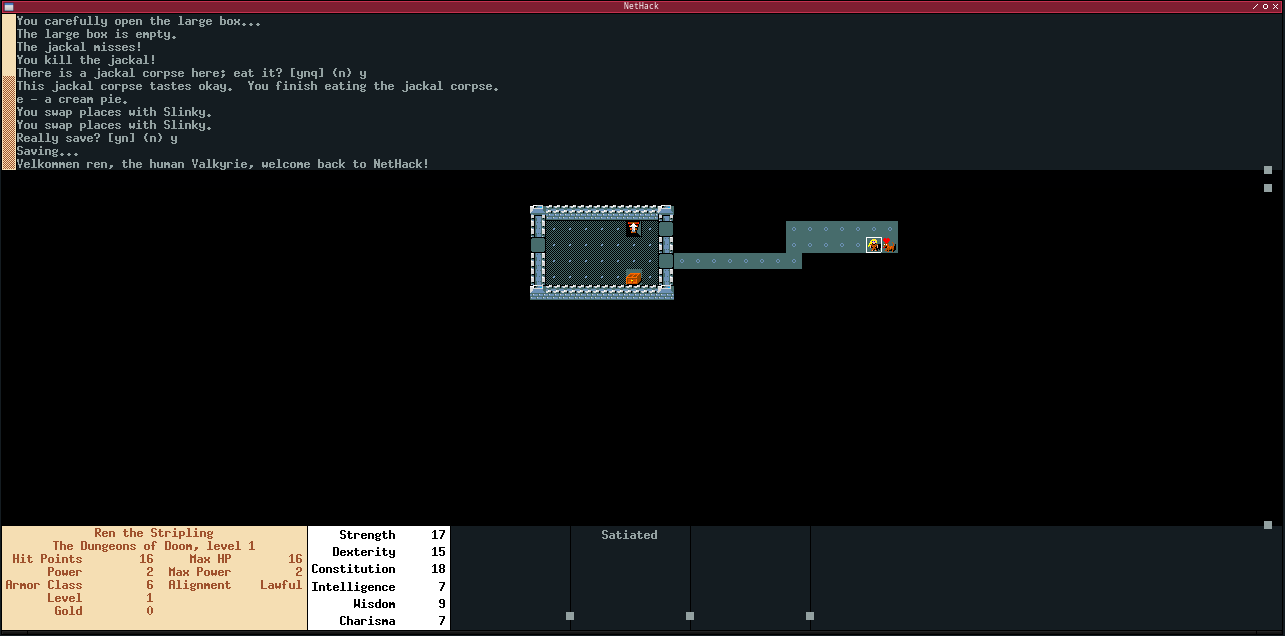
\includegraphics[height=.25\textwidth]{images/xnethack.png} 
    \\
    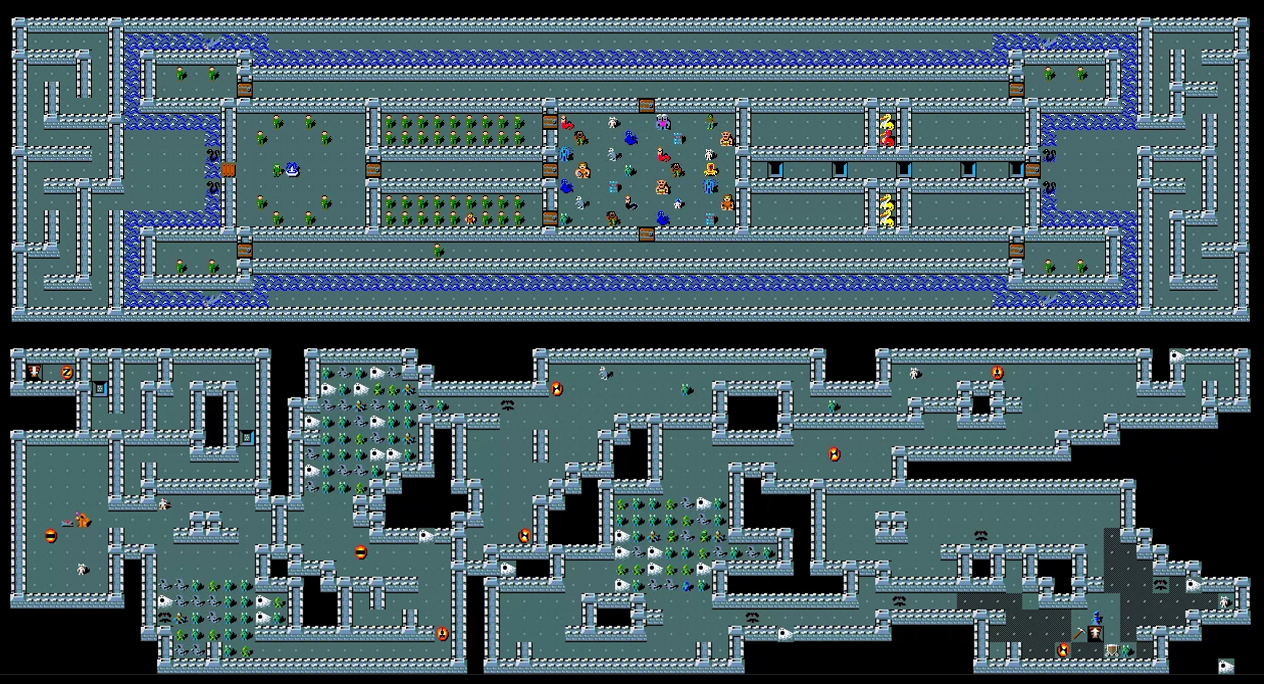
\includegraphics[width=.5\textwidth]{images/level_crop.png} 

\end{frame}


\begin{frame}[t]{1980s-1990s: GNU 与开源革命}
    \begin{itemize}
        \item \textbf{Richard Stallman 发起 GNU 项目} (1983)
        \item 自由软件基金会 (FSF) 成立 (1985)
    \end{itemize}
    \begin{figure}
        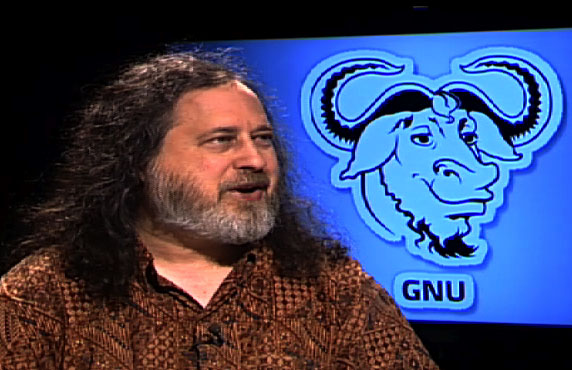
\includegraphics[width=0.7\textwidth]{images/stallman.jpg}
        \caption{Richard 与 GNU 项目}
    \end{figure}
\end{frame}

\begin{frame}[t]{1980s-1990s: GNU 与开源革命}
    \vspace{7em}
    \centering
    \Huge
    GNU: GNU's Not Unix
\end{frame}

\begin{frame}[t]{1980s-1990s: GNU 与开源革命}
  \begin{figure}
        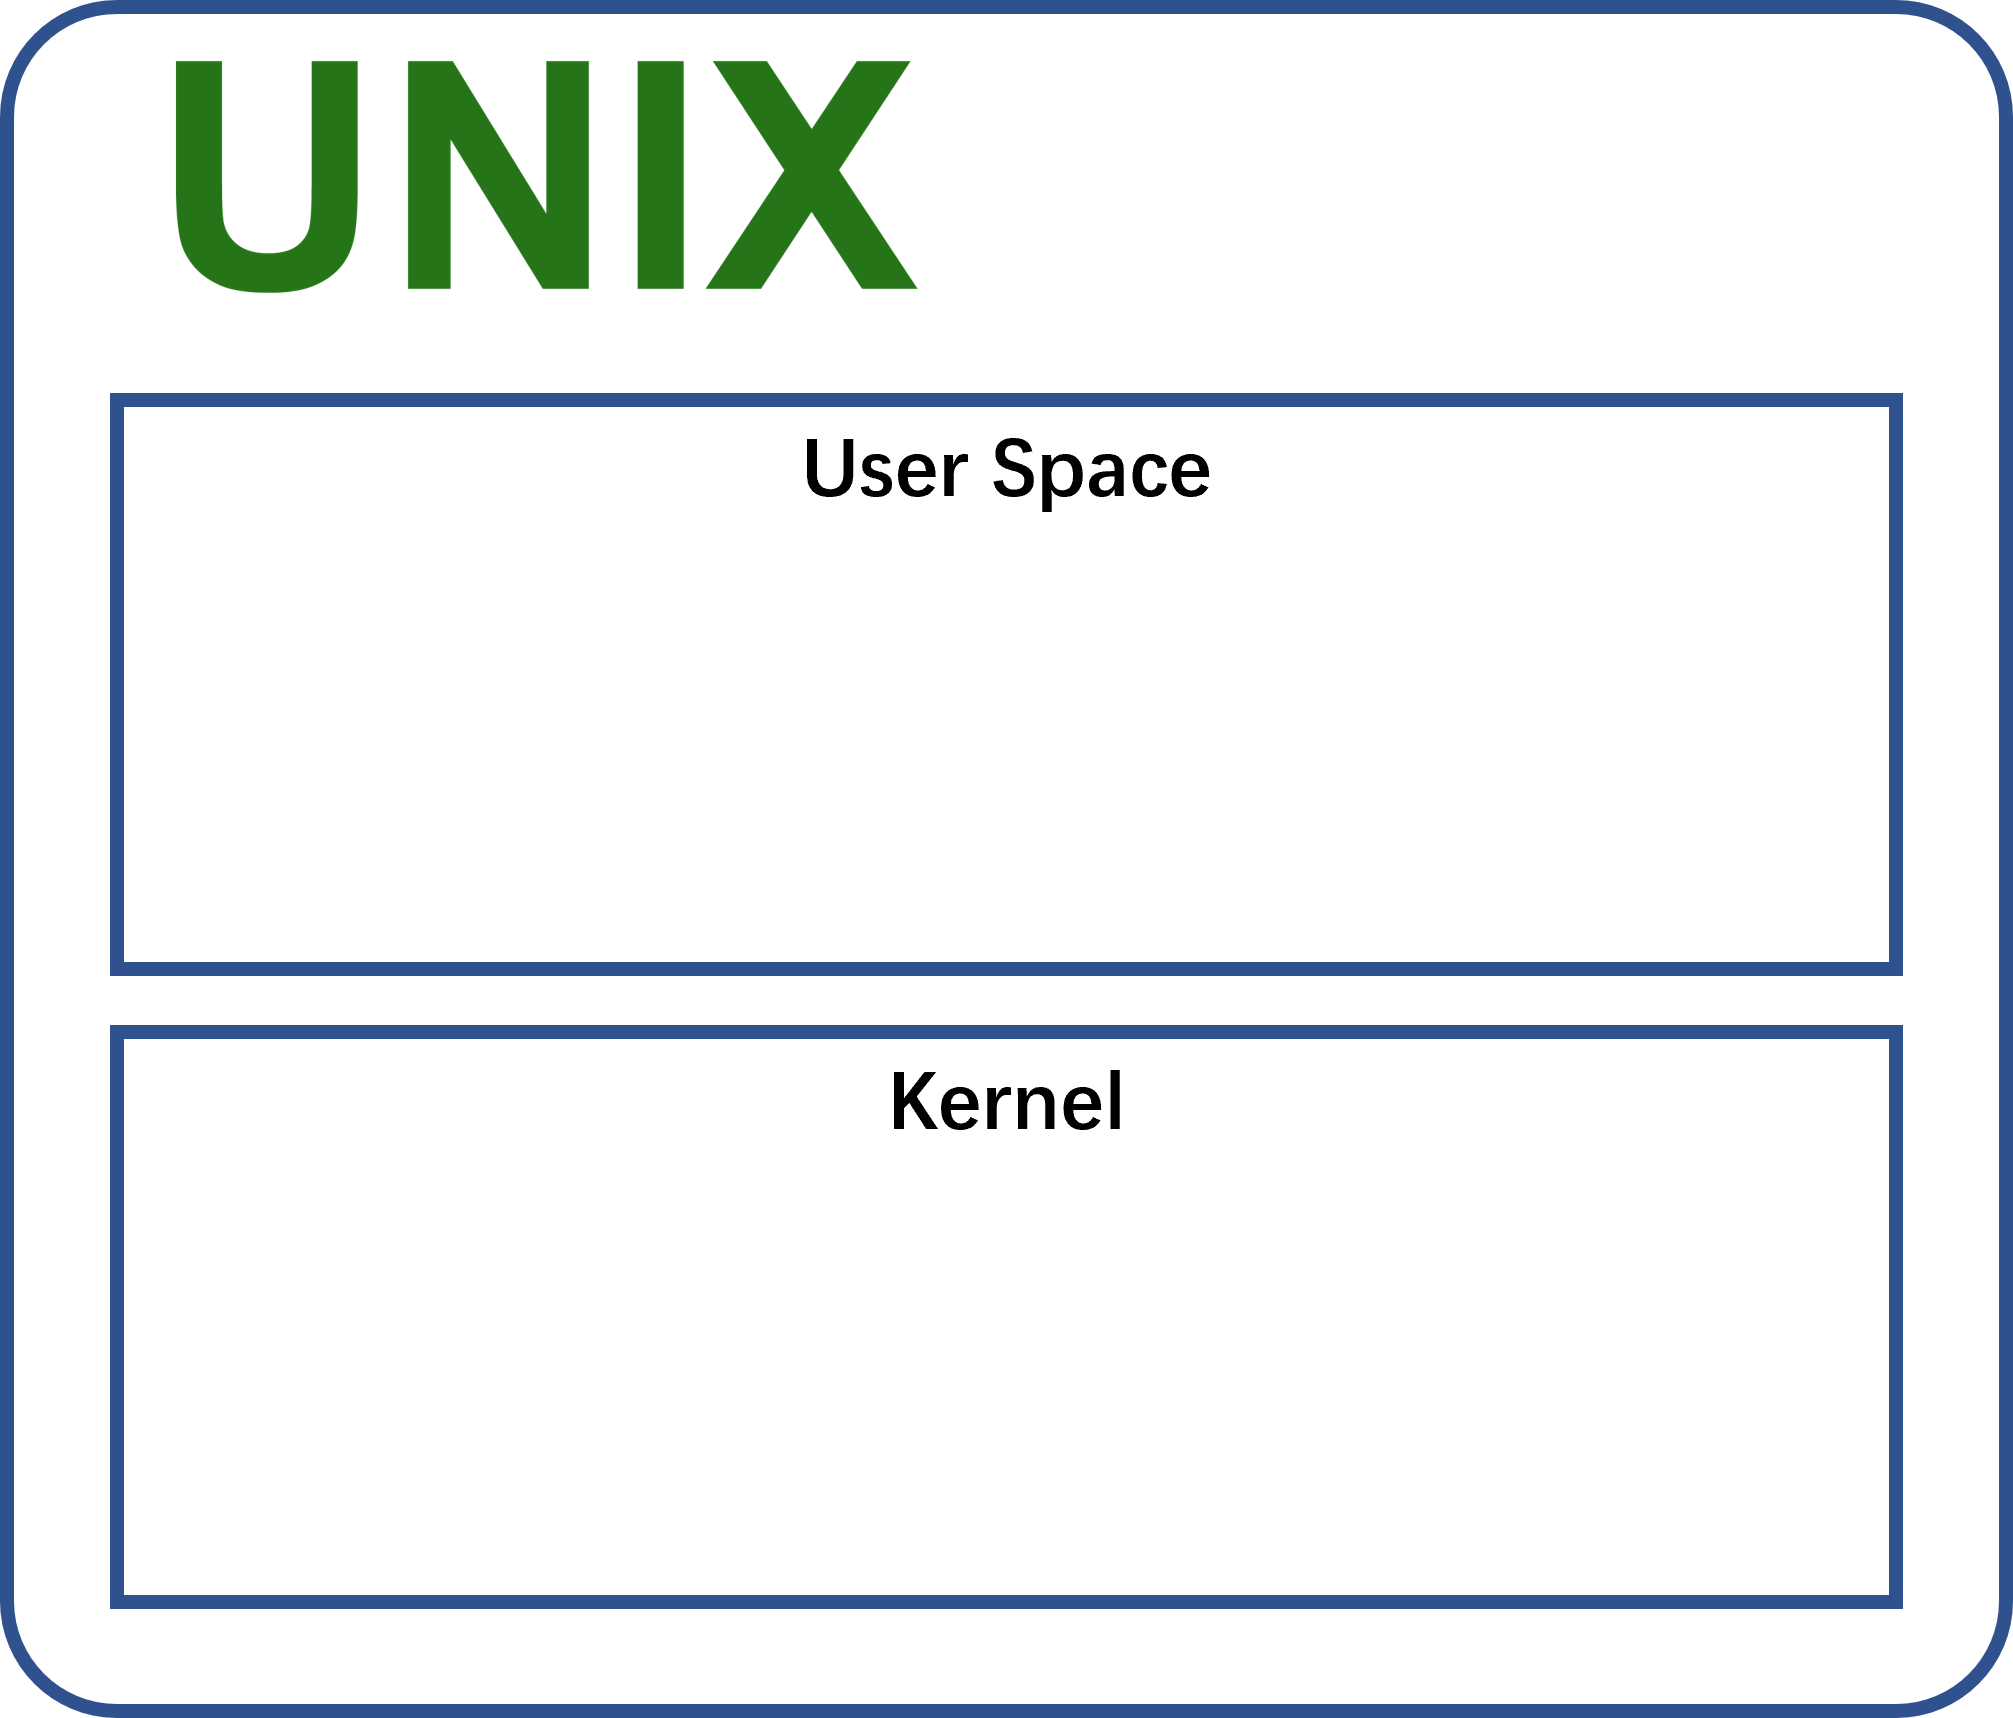
\includegraphics[width=0.6\textwidth]{images/gnu1.png}
        \caption{GNU 项目}
    \end{figure}
\end{frame}

\begin{frame}[t]{1980s-1990s: GNU 与开源革命}
    \begin{figure}
        
\includegraphics[width=0.6\textwidth]{images/gnu2.png}
        \caption{GNU 项目}
    \end{figure}
\end{frame}

\begin{frame}[t]{1980s-1990s: GNU 与开源革命}
    \begin{figure}
        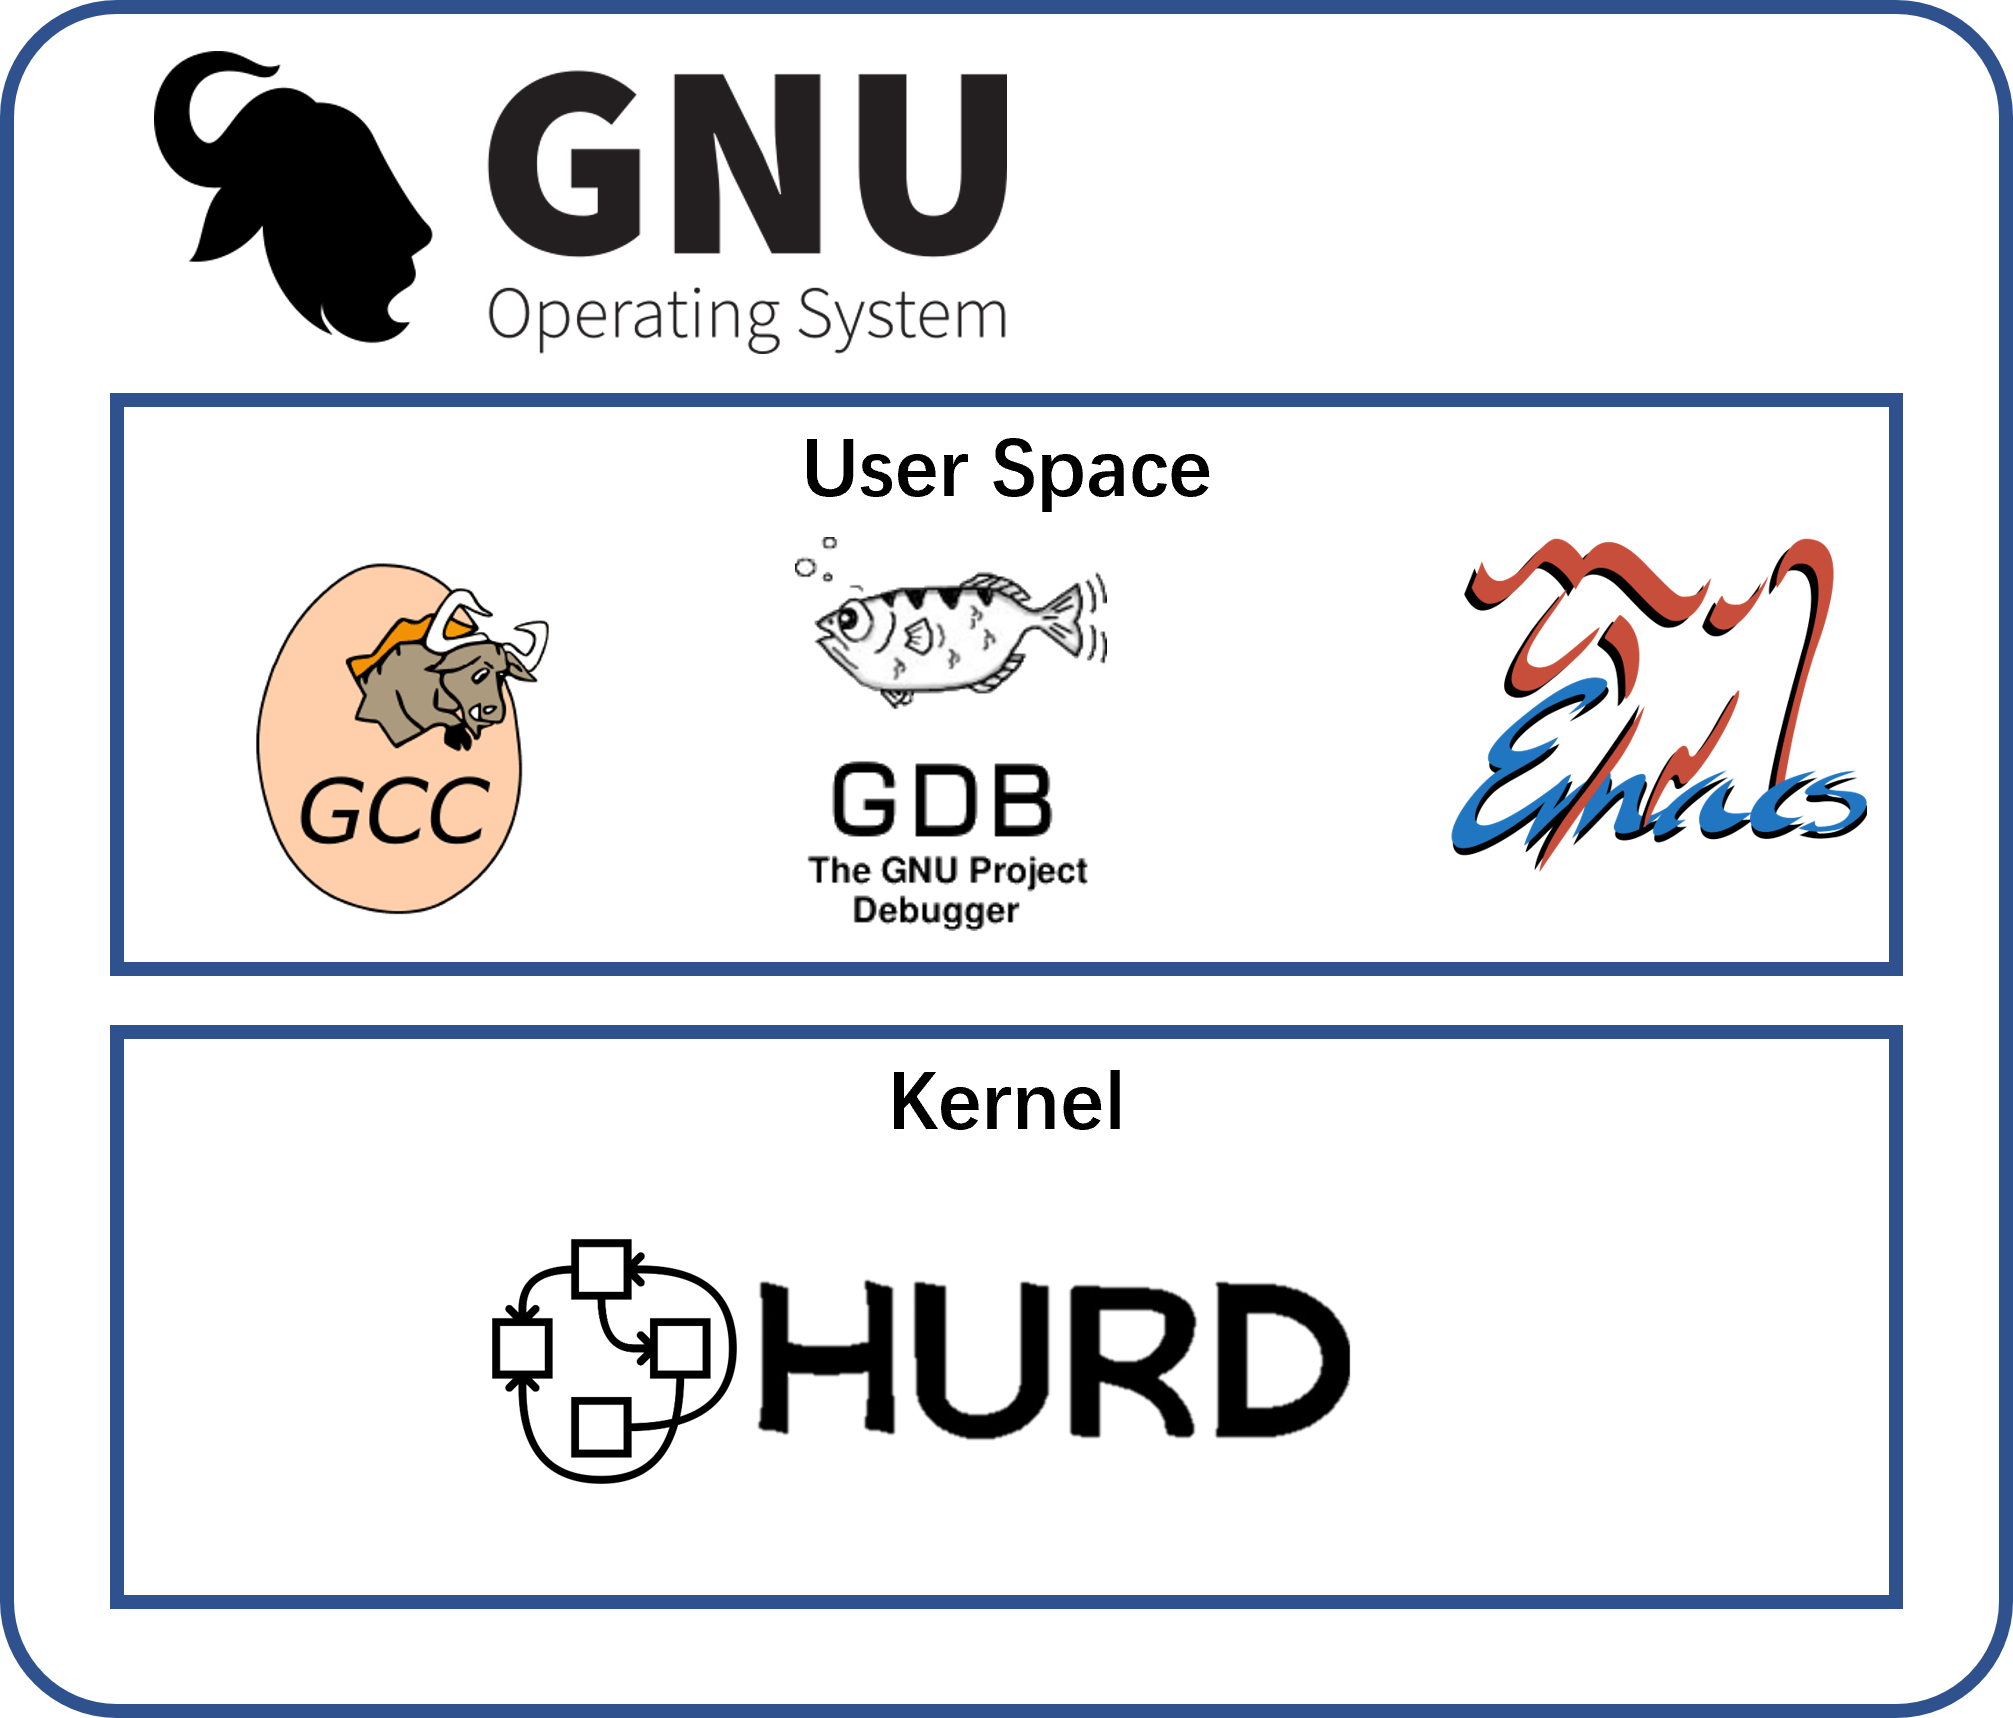
\includegraphics[width=0.6\textwidth]{images/gnu3.png}
        \caption{GNU 项目}
    \end{figure}
\end{frame}

\begin{frame}[t]{1980s-1990s: GNU 与开源革命}
    \begin{figure}
      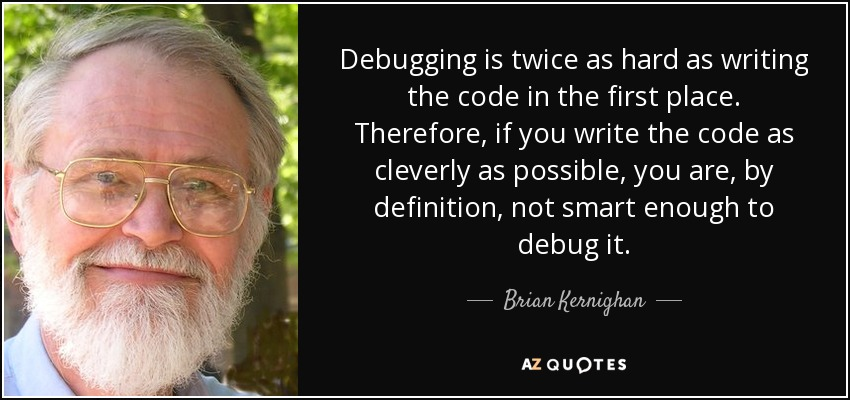
\includegraphics[width=0.8\textwidth]{images/quote-debugging.jpg}
        \caption{Brian Kernighan 谈调试}
    \end{figure}
\end{frame}

\begin{frame}[t]{1980s-1990s: GNU 与开源革命}
    \begin{figure}
        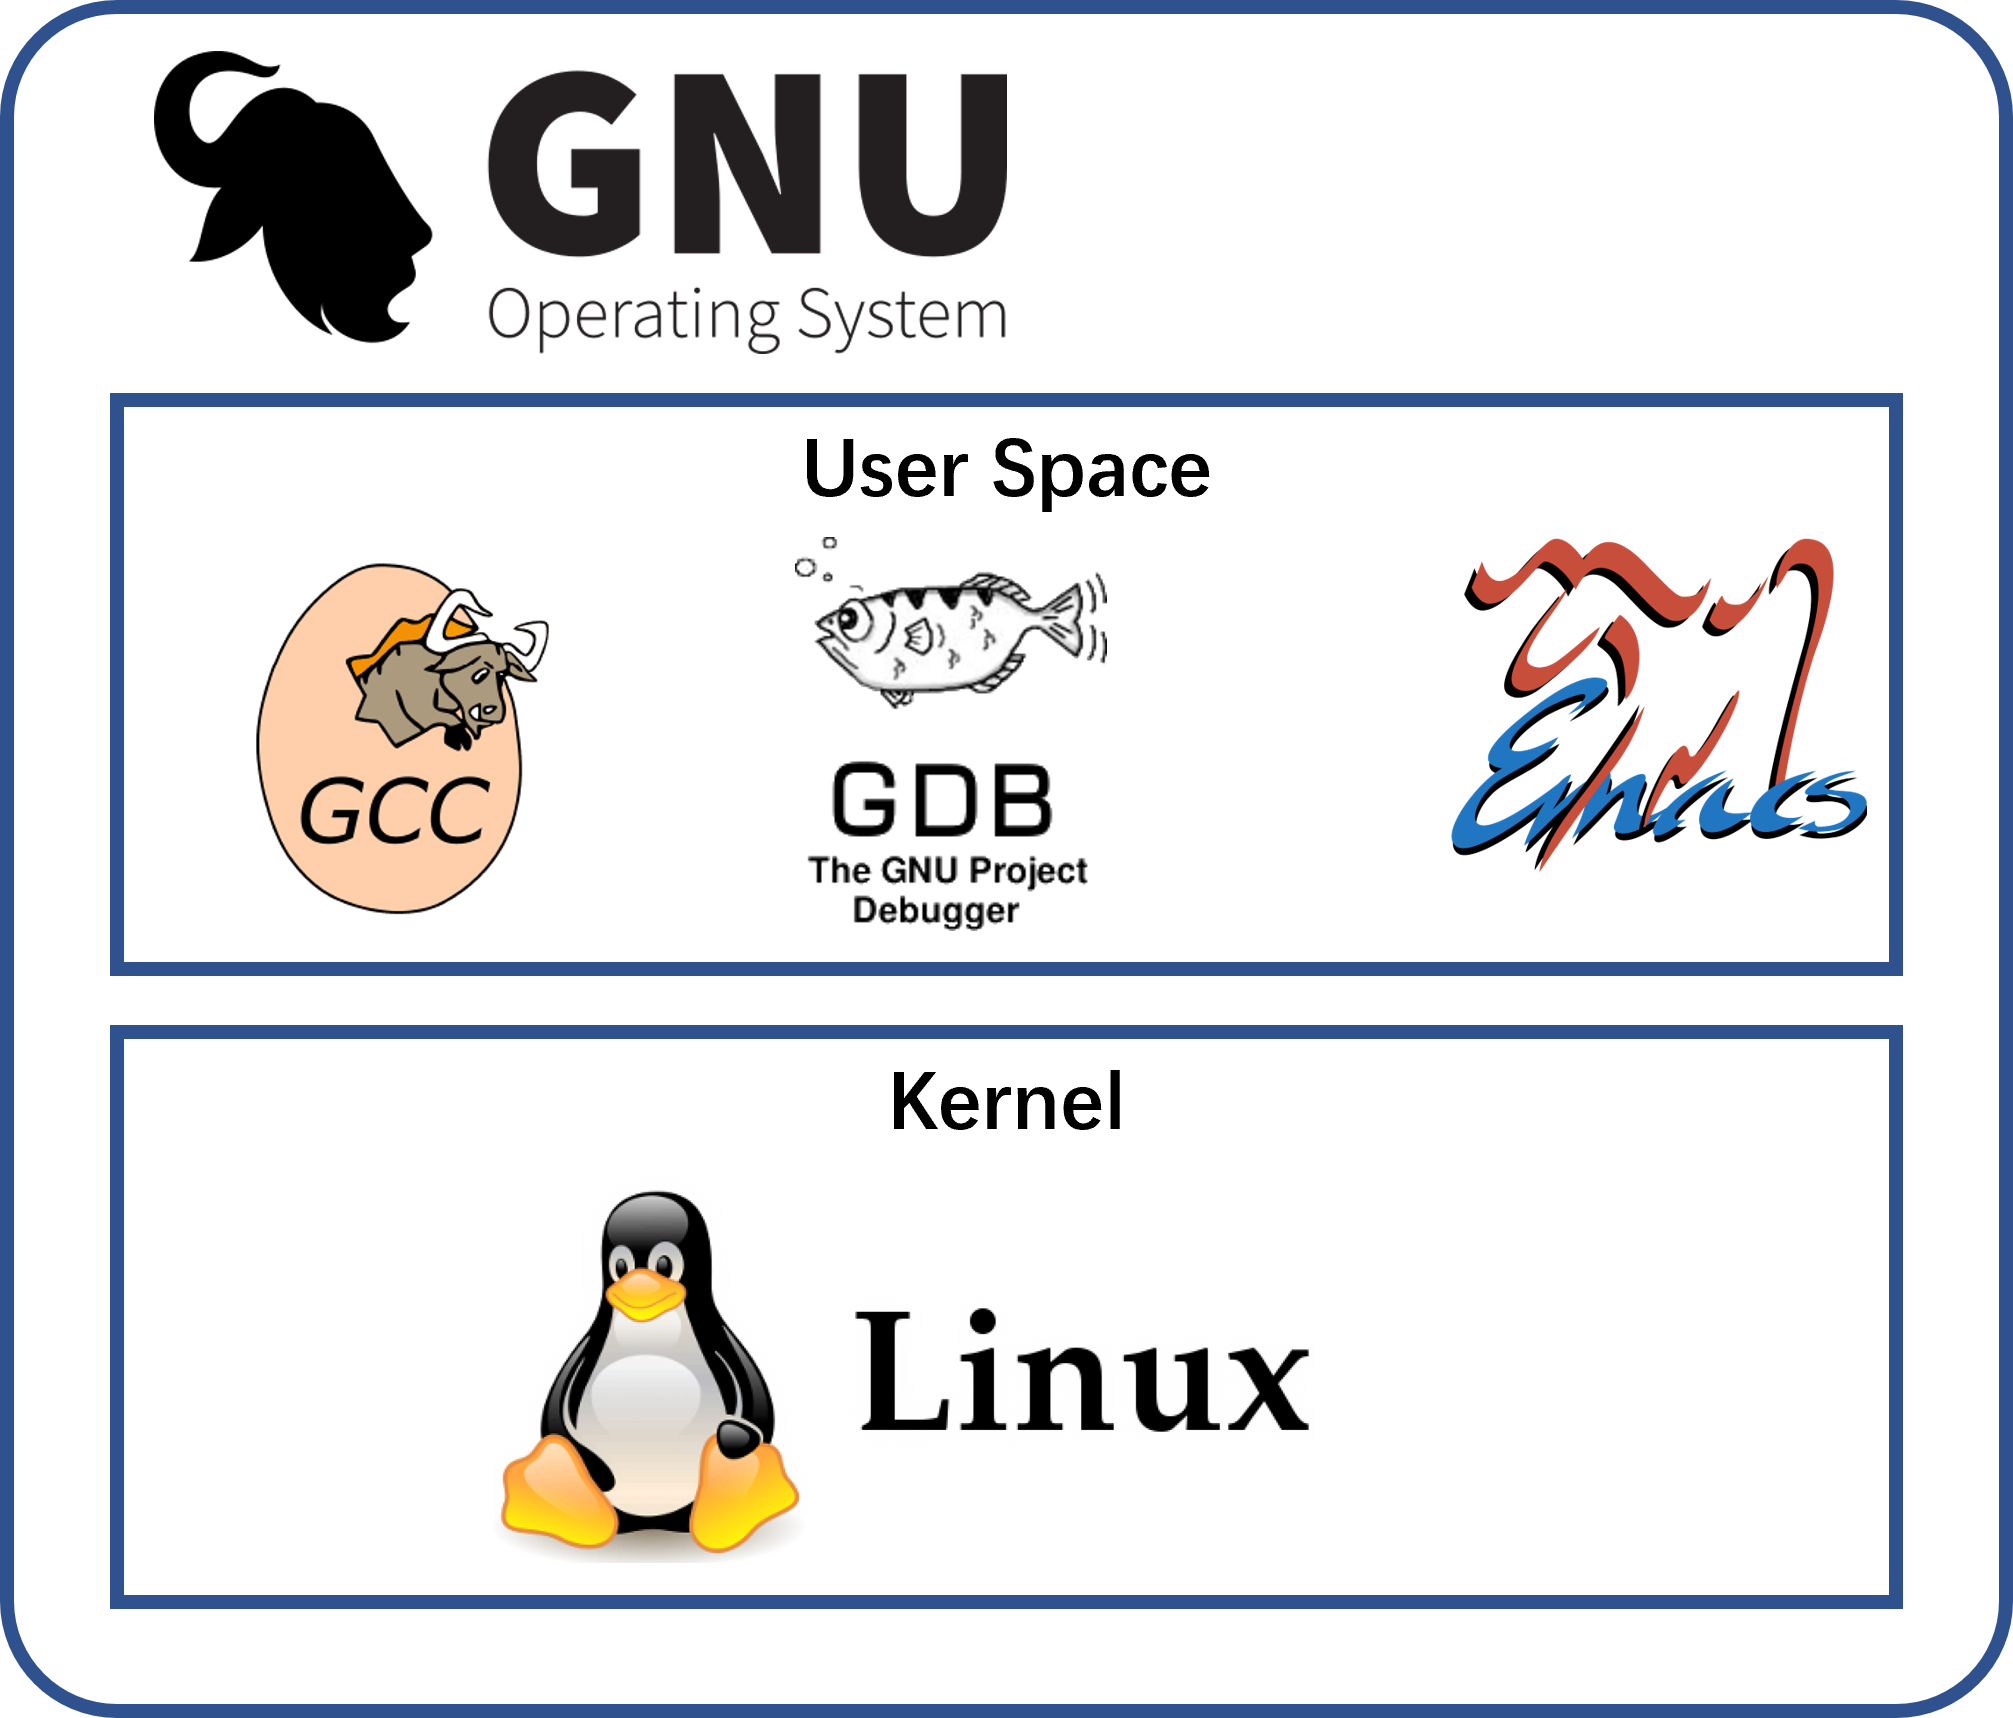
\includegraphics[width=0.6\textwidth]{images/gnu4.png}
        \caption{GNU 项目}
    \end{figure}
\end{frame}

\begin{frame}[t]{1980s-1990s: GNU 与开源革命}
    \begin{itemize}
        \item Linus Torvalds 创建 Linux 内核 (1991)
        \item 开源促进会 (OSI) 成立 (1998)
    \end{itemize}
    \begin{figure}
      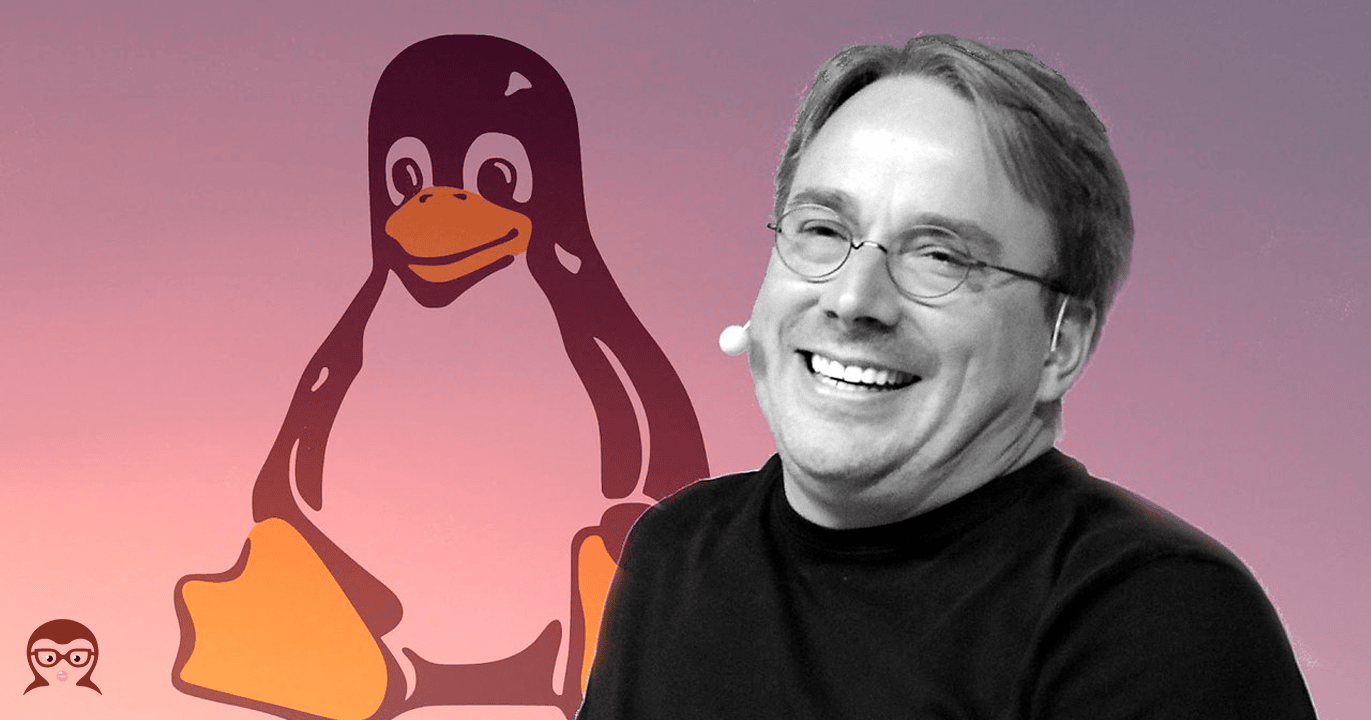
\includegraphics[width=0.8\textwidth]{images/Linus-Torvalds-Linux.png}
        \caption{Linus Torvalds 与 Linux}
    \end{figure}
\end{frame}

\begin{frame}[t]{从 Netscape 到 Firefox}
\begin{block}{巨人的陨落：Netscape 的“大教堂”}
\begin{itemize}
    \item \textbf{Netscape Navigator} 在1990年代中期曾占据90\%的市场份额。
    \item 在“第一次浏览器大战”中输给了微软的 Internet Explorer。
    \item 面对被淘汰的风险，Netscape 在 \textbf{1998年} 采取了激进的一步。
\end{itemize}
\end{block}
\end{frame}

\begin{frame}[t]{从 Netscape 到 Firefox}
    \begin{figure}
        \subfloat[]{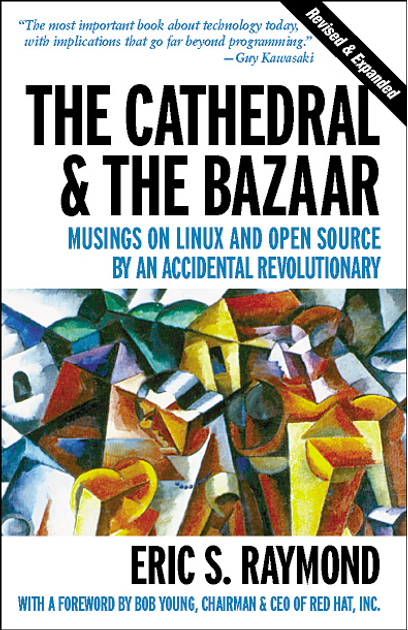
\includegraphics[height=4cm]{images/cathedral.png}}    
        \subfloat[]{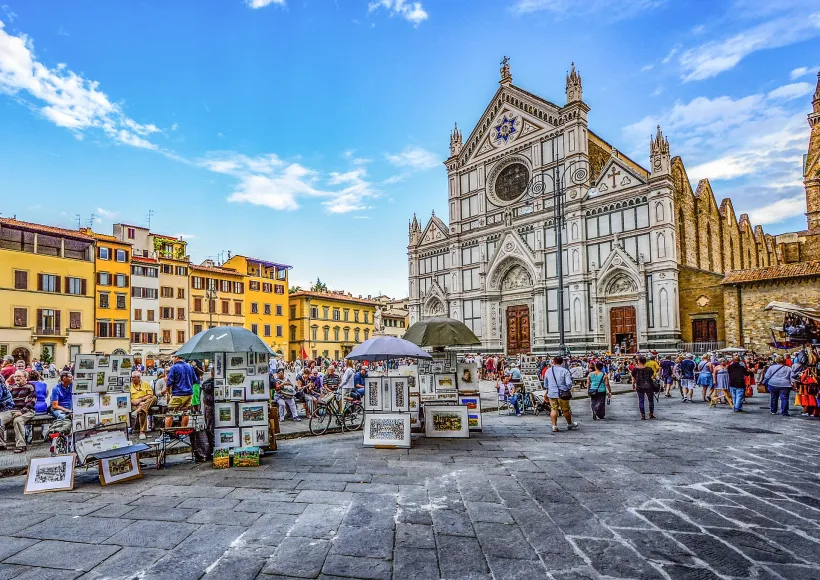
\includegraphics[height=4cm]{images/florence-1964638_1920.png}}    
        \caption{大教堂与市集 (The Cathedral and the Bazzar)}
    \end{figure}
\end{frame}

\begin{frame}[t]{从 Netscape 到 Firefox}
\begin{block}{激进转变：拥抱“市集”}
\begin{itemize}
    \item 1998年1月，Netscape 将其浏览器代码（Netscape Communicator 4.0）\textbf{开源}，以利用分布式开发者的力量。
    \item 成立了 \textbf{Mozilla 组织} 来管理该项目。
    \item 旧代码臃肿难用；开发者决定从零开始，使用新的 \textbf{Gecko} 渲染引擎。
\end{itemize}
\end{block}
\end{frame}

\begin{frame}[t]{从 Netscape 到 Firefox}
\begin{block}{凤凰涅槃：Firefox 的诞生}
\begin{itemize}
    \item 从 Mozilla 代码库中，诞生了一个名为 \textbf{Phoenix} (2002) 的轻量级、以用户为中心的浏览器。
    \item 经过商标争议（Phoenix $\rightarrow$ Firebird $\rightarrow$ \textbf{Firefox}），Mozilla Firefox 1.0 于 \textbf{2004年} 发布。
    \item Firefox 挑战了 IE 的垄断，捍卫了开放标准和用户选择权。
\end{itemize}
\end{block}
    \begin{figure}
        
\includegraphics[width=0.5\textwidth]{images/firefox-logo.jpg}
        \caption{Firefox Logo 演变}
    \end{figure}
\end{frame}

\begin{frame}[t]{哲学引擎：大教堂 vs. 市集}
\begin{columns}
    \begin{column}{0.48\textwidth}
        \begin{block}{大教堂模式}
            \scriptsize
            \begin{itemize}
                \item \textbf{封闭、集中的开发}。
                \item 由少数专门的专家团队构建。
                \item 版本发布周期长，是大规模的事件。
                \item \textbf{例子}：1998年之前的 Netscape，传统软件开发。
            \end{itemize}
        \end{block}
    \end{column}
    \begin{column}{0.48\textwidth}
        \begin{block}{市集模式}
            \scriptsize
            \begin{itemize}
                \item \textbf{开放、分散的开发}。
                \item 代码通过互联网公开开发。
                \item “只要眼睛足够多，所有 Bug 都会无所遁形。”
                \item \textbf{例子}：Mozilla, Linux, Firefox。
            \end{itemize}
        \end{block}
    \end{column}
\end{columns}
\vspace{1em}
\begin{exampleblock}{核心启示}
从 Netscape 到 Firefox 的故事表明，通过全球协作，管理良好的 \textbf{市集模式} 能够比封闭模式更有效地构建复杂的高质量系统。
\end{exampleblock}
\end{frame}

\begin{frame}[t]{遗产与深远影响}
\begin{itemize}
    \item \textbf{技术基础}：Gecko 引擎为 Firefox 铺平了道路。Netscape 的遗产还包括 JavaScript, SSL 和 Cookie。
    \item \textbf{机制化}：\textbf{Mozilla 基金会} (成立于2003年7月) 确保了项目使命超越了单一公司的寿命。
    \item \textbf{持久战}：Firefox 成为 IE 的主要替代品，证明了开源软件对主流用户的可行性。
\end{itemize}
\begin{center}
    \textbf{从大教堂灰烬中诞生的开源市集，帮助确保了互联网的开放性和竞争性。}
\end{center}
\end{frame}

\begin{frame}[t]
    \frametitle{趣味冷知识}
    \begin{itemize}
        \scriptsize
        \item Tøyen Cola: \url{https://distrita.com/toyen-cola-is-a-speciality-in-oslo-norway-that-needs-to-be-tested/}
        \item Open Soda: \url{http://www.opensoda.org/}
        \item Cube Cola: \url{https://cube-cola.org/}
    \end{itemize}
    \begin{figure}
        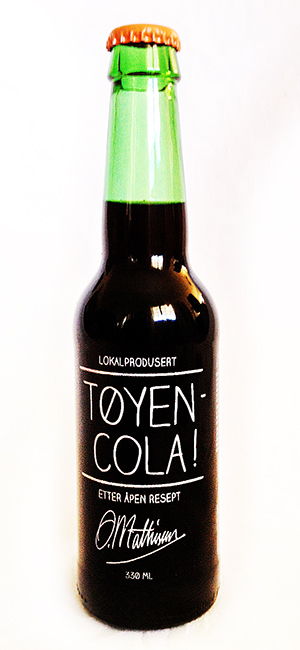
\includegraphics[width=0.2\textwidth]{images/cola.jpg}
    \caption{开源可乐}
    \end{figure}
\end{frame}

\begin{frame}[t]
    \frametitle{趣味冷知识}
    \begin{itemize}
        \scriptsize
        \item 开源硬件由开放设计运动所设计和提供的技术实体组成
        \item 硬件设计（如机械图、电路图、物料清单、PCB布局数据、HDL源码和集成电路布局数据）以及驱动硬件的软件，全部在自由/开放条款下发布
    \end{itemize}
    \begin{figure}
        
\includegraphics[width=0.2\textwidth]{images/arduino.png}
        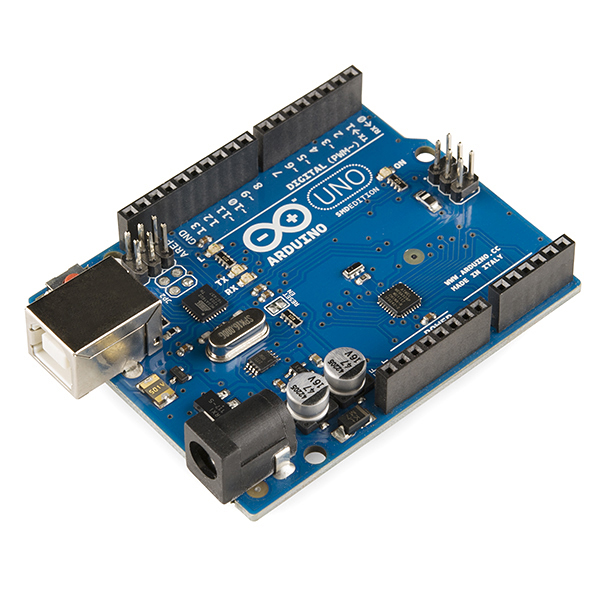
\includegraphics[width=0.2\textwidth]{images/Arduino_Uno.jpg}
    \caption{开源硬件}
    \end{figure}
\end{frame}

\begin{frame}[t]{1980s-1990s: 面向对象革命}
\begin{itemize}
    \item \textbf{Smalltalk} (1970s-1980s)：纯面向对象 (OOP) 概念
    \item \textbf{C++} (1985)：将 OOP 引入系统级编程
    \item \textbf{Java} (1995)：“一次编写，到处运行”
    \item 核心原则：封装、继承、多态
    \item 设计模式（Gang of Four 著作, 1994）
\end{itemize}
\begin{figure}
    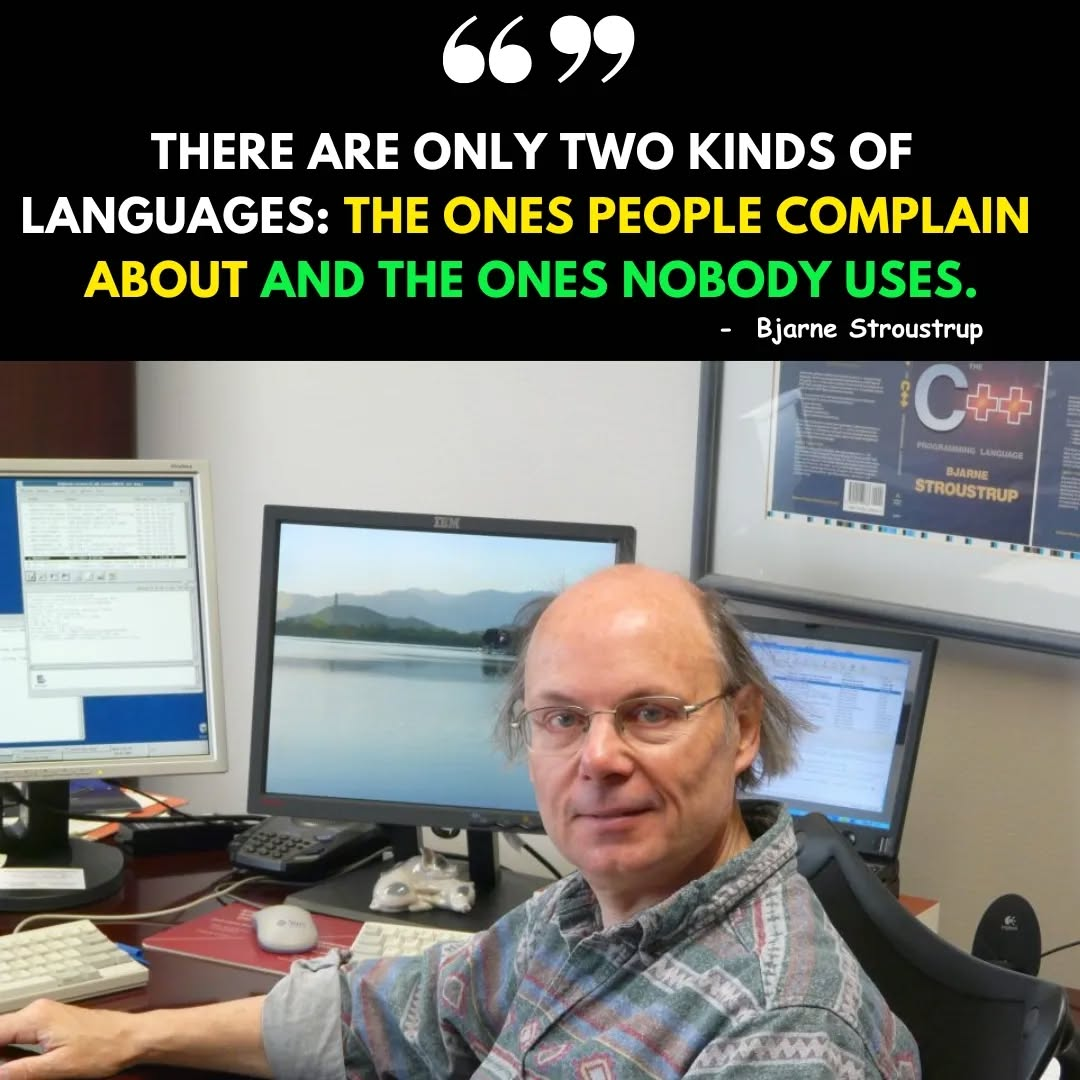
\includegraphics[width=0.3\textwidth]{images/cpp.jpeg}
    \caption{C++ 创始人的语录}
\end{figure}
\end{frame}

\subsection{现代时期}

\begin{frame}[t]{2000s: 敏捷与 DevOps}
    \begin{itemize}
        \item \textbf{敏捷宣言} (2001)：强调迭代开发和客户协作
        \item \textbf{DevOps 运动} (2000年代末)
        \item 弥合开发与运维的鸿沟，以 Git 和 CI/CD 为特征
        \item 基础设施即代码 (IaC)
    \end{itemize}
    \begin{figure}
        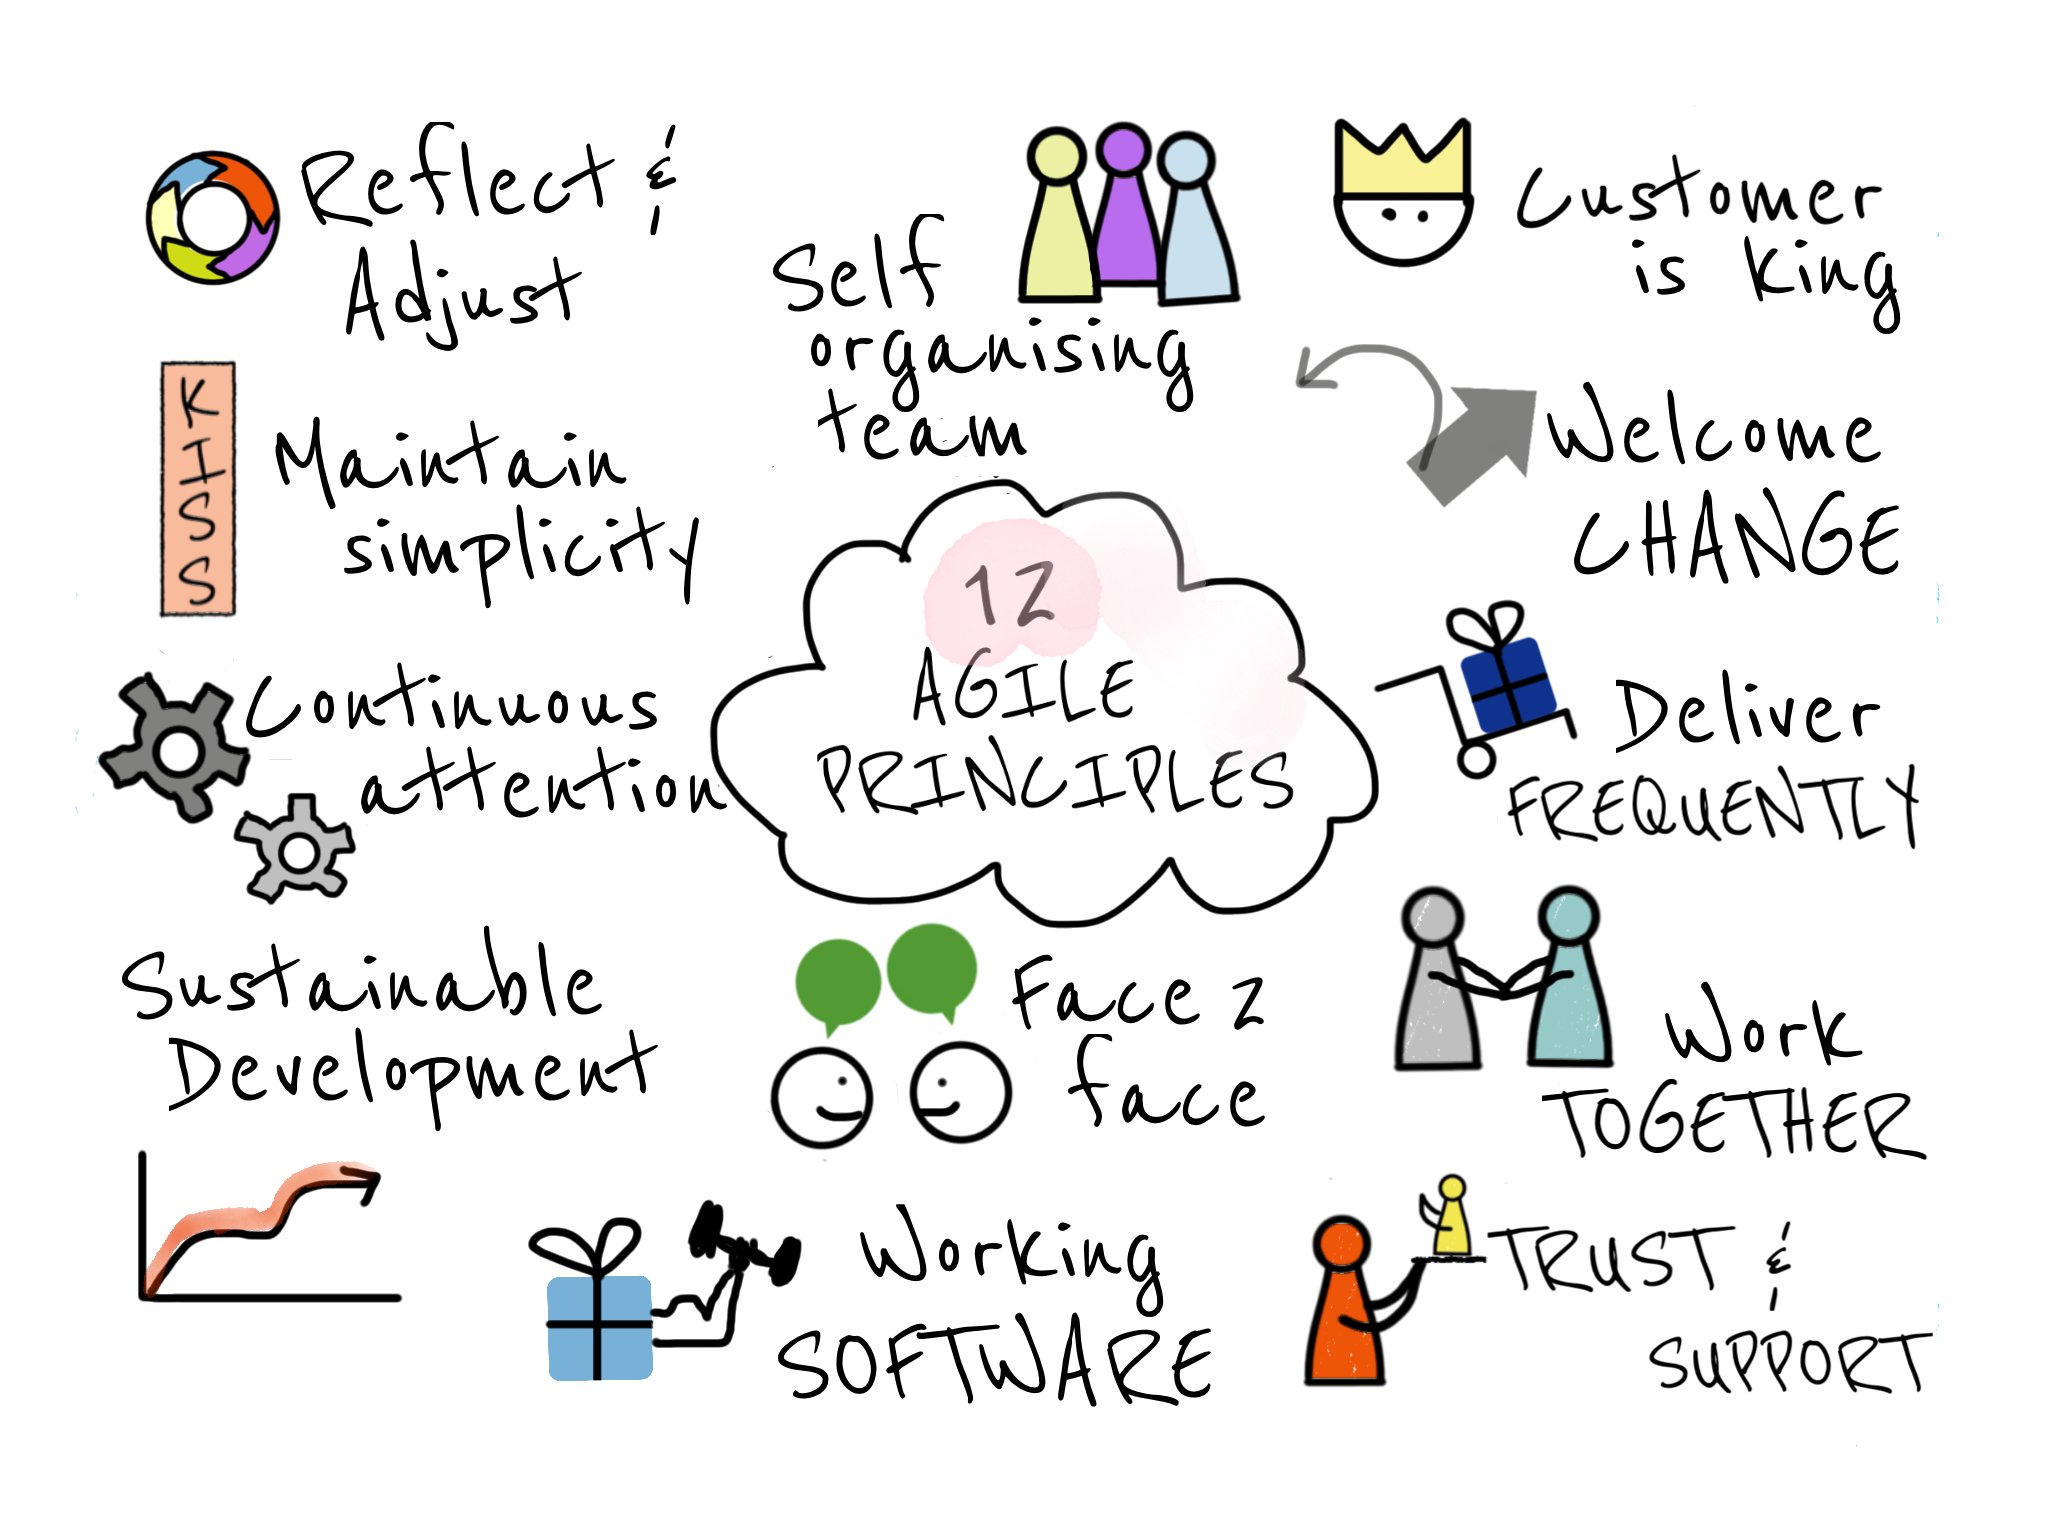
\includegraphics[width=0.3\textwidth]{images/agile-manifesto.png}
        \caption{敏捷12条原则}
    \end{figure}
\end{frame}

\begin{frame}[t]{1990s: CVS - 并发版本系统}
\begin{columns}
    \begin{column}{0.6\textwidth}
      \begin{itemize}
            \item \textbf{开发于1986年}，在1990年代占据主导地位
            \item \textbf{集中式架构}：单一中央仓库
            \item \textbf{关键功能}：
                \begin{itemize}
                    \item 基础版本追踪
                    \item 支持多开发者
                    \item 基于网络的访问
                \end{itemize}
            \item \textbf{局限性}：
                \begin{itemize}
                    \item 缺乏原子提交
                    \item 分支/合并功能差
                    \item 网络操作缓慢
                    \item 单点故障风险
                \end{itemize}
        \end{itemize}
    \end{column}
    \begin{column}{0.4\textwidth}
        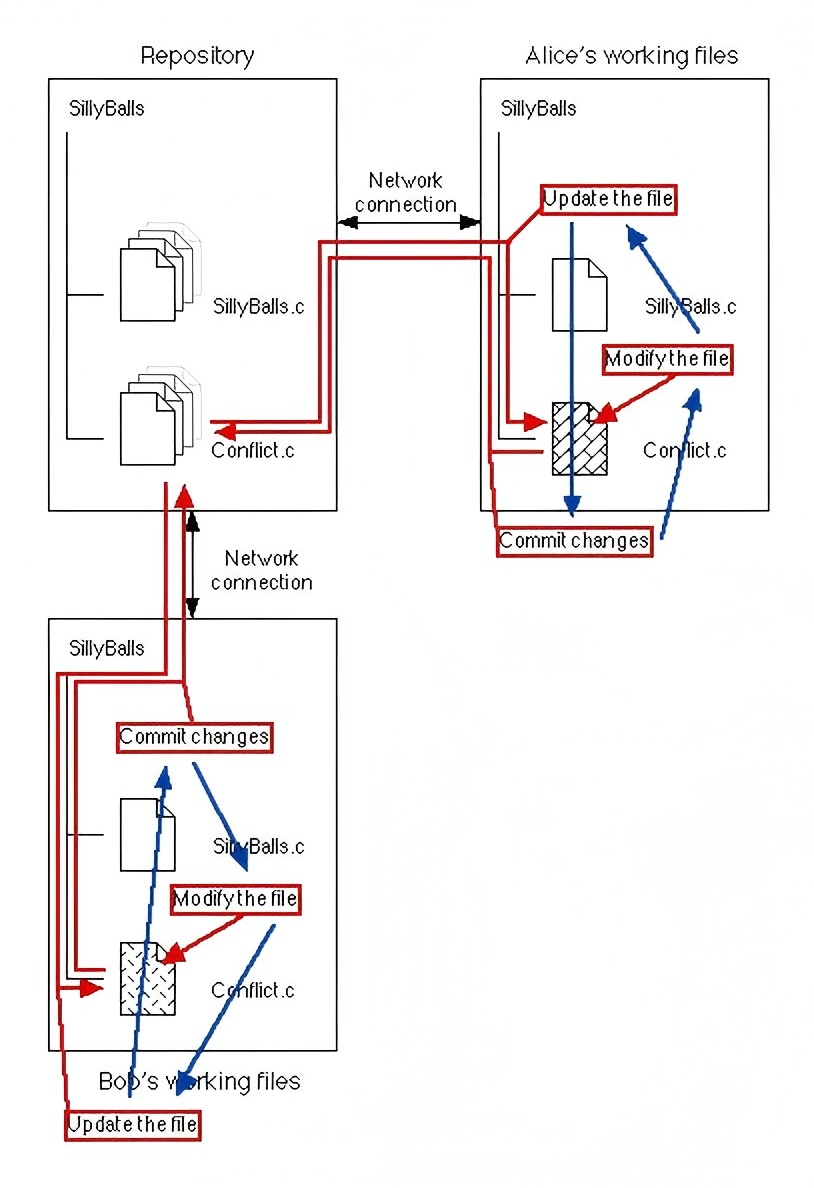
\includegraphics[width=0.9\textwidth]{images/cvs.jpg}
        \\\scriptsize{CVS 集中式架构}
    \end{column}
\end{columns}
\begin{block}{}
CVS 将版本控制带给了大众，但协作过程是顺序且谨慎的。
\end{block}
\end{frame}

\begin{frame}[t]{2000: Subversion - “正确的 CVS”}
\begin{itemize}
    \item \textbf{2000年创建}，旨在修复 CVS 的局限性
    \item \textbf{相比 CVS 的改进}：
        \begin{itemize}
            \item \textbf{原子提交}：更改要么全部成功，要么全部失败
            \item \textbf{更好的分支/标记}：廉价的复制操作
            \item \textbf{版本化的目录和重命名}
            \item \textbf{更好的二进制文件处理}
        \end{itemize}
    \item \textbf{依然是集中式}：单一仓库模型
    \item \textbf{采用情况}：迅速成为企业标准
    \item \textbf{局限性}：中央服务器 = 单点故障，离线工作困难
\end{itemize}
\end{frame}

\begin{frame}[t]{2002-2005: BitKeeper 争议}
        \begin{itemize}
            \item \textbf{Linux 内核开发}规模超出了基于补丁的工作流
            \item \textbf{BitKeeper}：专有的分布式版本控制系统
            \item \textbf{2002年被 Linux 采用}：实现了真正的分布式开发
            \item \textbf{革命性功能}：
                \begin{itemize}
                    \item 分布式仓库
                    \item 卓越的分支/合并功能
                    \item 快速的性能
                \end{itemize}
            \item \textbf{争议 (2005)}：许可协议纠纷导致 BitKeeper 停止免费提供
            \item \textbf{催化剂}：迫使 Linux 社区创建自己的解决方案
        \end{itemize}
\end{frame}

\begin{frame}[t]{2005: Git - Linux 社区的回答}
\begin{itemize}
    \item \textbf{2005年由 Linus Torvalds 创建}，紧随 BitKeeper 争议之后
        \begin{itemize}
            \item 分布式且点对点
            \item 强大的加密完整性 (SHA-1)
            \item 快速的分支/合并
            \item 高效处理大型项目
            \item 支持非线性开发
        \end{itemize}
    \item \textbf{关键创新}：
      \begin{itemize}
            \item 内容寻址存储
            \item 基于有向无环图 (DAG) 的历史记录
            \item 三阶段思维（工作目录、暂存区、仓库）
        \end{itemize}
\end{itemize}
\begin{center}
    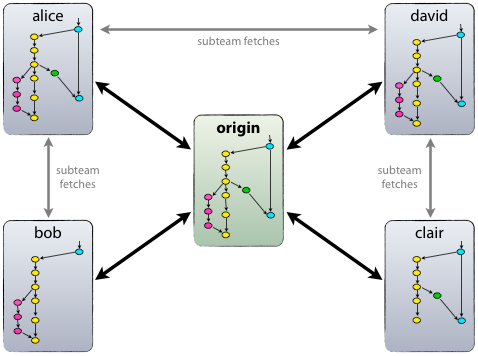
\includegraphics[width=0.3\textwidth]{images/git-dist.png}
\end{center}
\end{frame}

\begin{frame}[t]{xkcd 谈 Git}
    \begin{figure}
        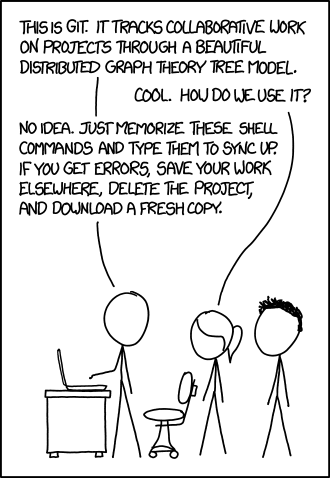
\includegraphics[width=0.3\textwidth]{images/git.png}
        \caption{Git 漫画}
    \end{figure}
\end{frame}

\begin{frame}[t]{为什么 Git 赢了：分布式工作流}
\begin{columns}
    \begin{column}{0.5\textwidth}
        \textbf{集中式 (CVS/SVN)}
        \begin{itemize}
            \item 单一信任源
            \item 顺序提交
            \item 必须联网
            \item 分支成本高
            \item 线性历史
        \end{itemize}
    \end{column}
    \begin{column}{0.5\textwidth}
        \textbf{分布式 (Git)}
        \begin{itemize}
            \item 每个克隆都是完整仓库
            \item 并行开发
            \item 离线工作，随后同步
            \item 廉价分支
            \item 非线性历史
        \end{itemize}
    \end{column}
\end{columns}
\begin{block}{游戏规则改变者}
Git 实现了诸如 \textbf{功能分支 (feature branching)} 和 \textbf{拉取请求 (pull requests)} 的工作流，使开源协作具有可扩展性。
\end{block}
\end{frame}

\begin{frame}[t]{GitHub 与社交编程革命 (2008)}
\begin{itemize}
    \item \textbf{GitHub 2008年上线}：为 Git 添加了社交层
    \item \textbf{关键创新}：
        \begin{itemize}
            \item 拉取请求 (Pull Request)：代码审查成为一等公民
            \item Fork \& Pull 模型：轻松贡献任何项目
            \item Issue、项目看板、Wiki：集成化的项目管理
        \end{itemize}
    \item \textbf{网络效应}：使开源协作成为主流
    \item \textbf{企业采用}：GitHub Enterprise, GitLab, Bitbucket
\end{itemize}
\end{frame}

\begin{frame}[t]{Git 赋能的 CI/CD：自动化革命}
\begin{itemize}
    \item \textbf{持续集成 (CI)}：自动构建并测试每一次提交
    \item \textbf{持续部署/交付 (CD)}：自动部署通过测试的代码
    \item \textbf{Git 作为触发器}： 
        \begin{itemize}
            \item 推送到仓库触发自动化流水线
            \item 分支保护规则强制执行质量关卡
            \item 拉取请求状态检查防止引入 Bug
        \end{itemize}
    \item \textbf{关键工具}：Jenkins, GitHub Actions, GitLab CI, CircleCI
\end{itemize}
\end{frame}

\begin{frame}[t]{演变时间线}
\begin{center}
    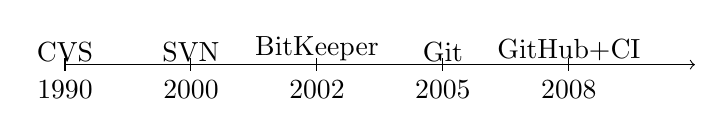
\begin{tikzpicture}[scale=0.8]
        \draw[->] (0,0) -- (10,0);
        \foreach \x/\year/\text in {0/1990/CVS, 2/2000/SVN, 4/2002/BitKeeper, 6/2005/Git, 8/2008/GitHub+CI/CD}
            \draw (\x,0.1) -- (\x,-0.1) node[below] {\year} node[above] {\text};
    \end{tikzpicture}
\end{center}

\begin{itemize}
    \item \textbf{1990s}：集中式时代 - 顺序协作
    \item \textbf{2000s}：集中式改良 - 更好但仍受限
    \item \textbf{2002-2005}：分布式觉醒 - BitKeeper 展示了方向
    \item \textbf{2005+}：Git 革命 - 并行、分布式协作
    \item \textbf{2008+}：社交编程 + 自动化 - CI/CD 生态
\end{itemize}
\end{frame}

\begin{frame}[t]{2010s: AIOps 与云原生}
\begin{itemize}
    \item \textbf{AIOps}：将人工智能应用于运维
    \begin{itemize}
        \item 自动化监控和事件响应
        \item 预测系统性能分析
        \item 异常检测与根因分析
    \end{itemize}
    \item \textbf{云原生开发}
    \begin{itemize}
        \item 微服务架构
        \item 容器化 (Docker, Kubernetes)
        \item 无服务器计算 (Serverless)
    \end{itemize}
\end{itemize}
\end{frame}

\subsection{LLM 时代}

\begin{frame}[t]{2020s: LLM 革命}
    \begin{itemize}
        \item \textbf{大语言模型改变软件工程}
        \item GitHub Copilot (2021) 及类似工具
    \end{itemize}
    \begin{figure}
        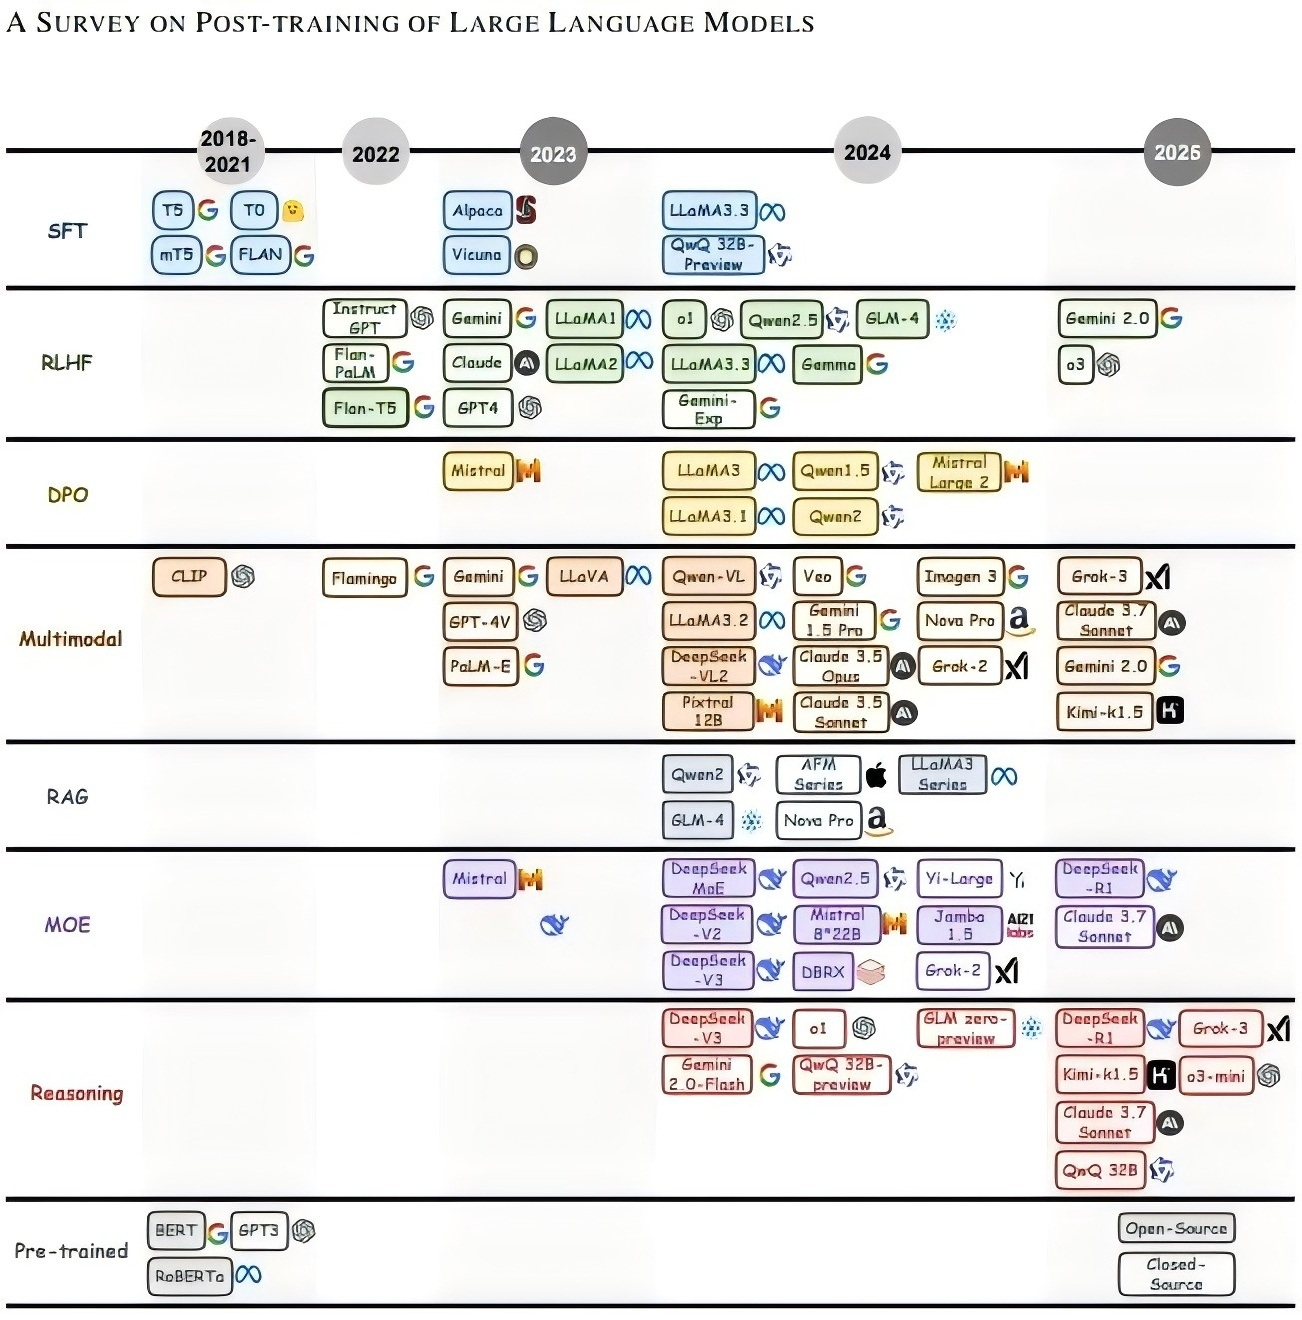
\includegraphics[width=0.5\textwidth]{images/timeline.jpg}
        \caption{LLM 发展时间线}
    \end{figure}
\end{frame}

\begin{frame}[t]{LLM 对软件工程的影响}
\begin{itemize}
    \item \textbf{代码生成}：从自动补全到生成整个函数
    \item \textbf{调试辅助}：AI 驱动的 Bug 检测与修复
    \item \textbf{文档自动化}：自动生成文档
    \item \textbf{代码审查}：AI 辅助的质量保证
    \item \textbf{测试}：智能测试用例生成
\end{itemize}
\begin{block}{未来方向}
\begin{itemize}
    \item AI 结对编程成为标准
    \item 新的编程范式正在出现
    \item 重心转向提示工程 (Prompt Engineering) 和 AI 监管
\end{itemize}
\end{block}
\end{frame}

\subsection{结论}

\begin{frame}[t]{展望未来}
\begin{itemize}
    \item 从严谨的工程化到 AI 增强的持续演进
    \item 越来越强调自动化和智能化
    \item 人为因素在系统设计和监管中依然至关重要
    \item AI 很强大，但它既不是银弹也不是万灵药
\end{itemize}
\begin{center}
    \textbf{旅程仍在继续...}
\end{center}
\end{frame}

\section{人工智能简史}
\subsection{先驱思想}
\begin{frame}[t]{构思的种子}
    \begin{itemize}
        \item \textbf{Ada Lovelace (1843)}：质疑机器是否能产生原创想法，还是只能执行人类的命令。
        \item \textbf{20世纪早期}：Karel Čapek 的剧本《R.U.R.》(1920) 创造了“robot”（机器人）一词。
    \end{itemize}

    \begin{figure}
        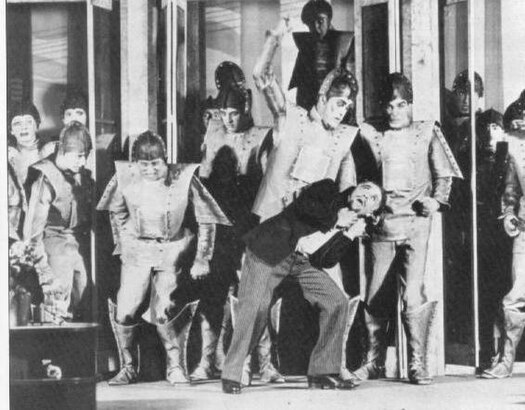
\includegraphics[width=0.3\textwidth]{images/Capek_RUR.jpg}
        \caption{Capek 的剧本 R.U.R}
    \end{figure}
\end{frame}

\subsection{1950s: 领域诞生}

\begin{frame}[t]{1950s: 奠基的十年}
    \begin{itemize}
        \item \textbf{Alan Turing (1950)}：发表《计算机器与智能》，提出 \textbf{图灵测试}。
    \end{itemize}
    \begin{figure}
        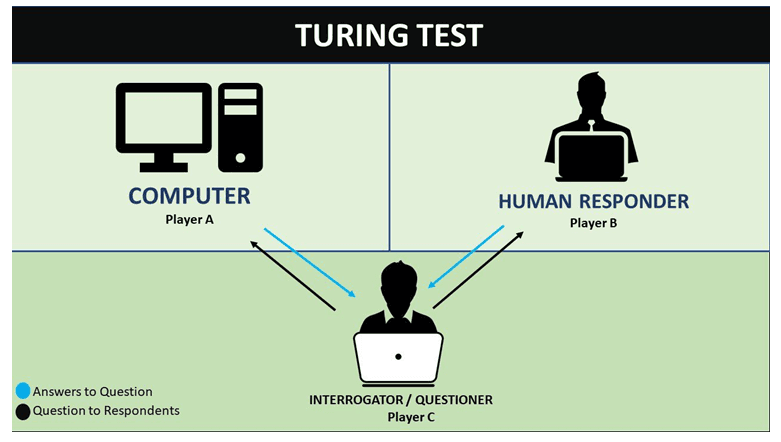
\includegraphics[width=0.7\textwidth]{images/turing-test.png}
        \caption{图灵测试示意图}
    \end{figure}
\end{frame}

\begin{frame}[t]{1950s: 奠基的十年}
    \begin{itemize}
        \item \textbf{术语诞生}：John McCarthy 组织了 \textbf{达特茅斯会议} (1956) 并创造了“人工智能 (Artificial Intelligence)”一词。
    \item \textbf{设定目标}：“学习的每一个方面或智能的任何其他特征，在原则上都可以被精确地描述，从而可以制造出一台机器来模拟它。” - 达特茅斯提案
    \end{itemize}
    \begin{figure}
        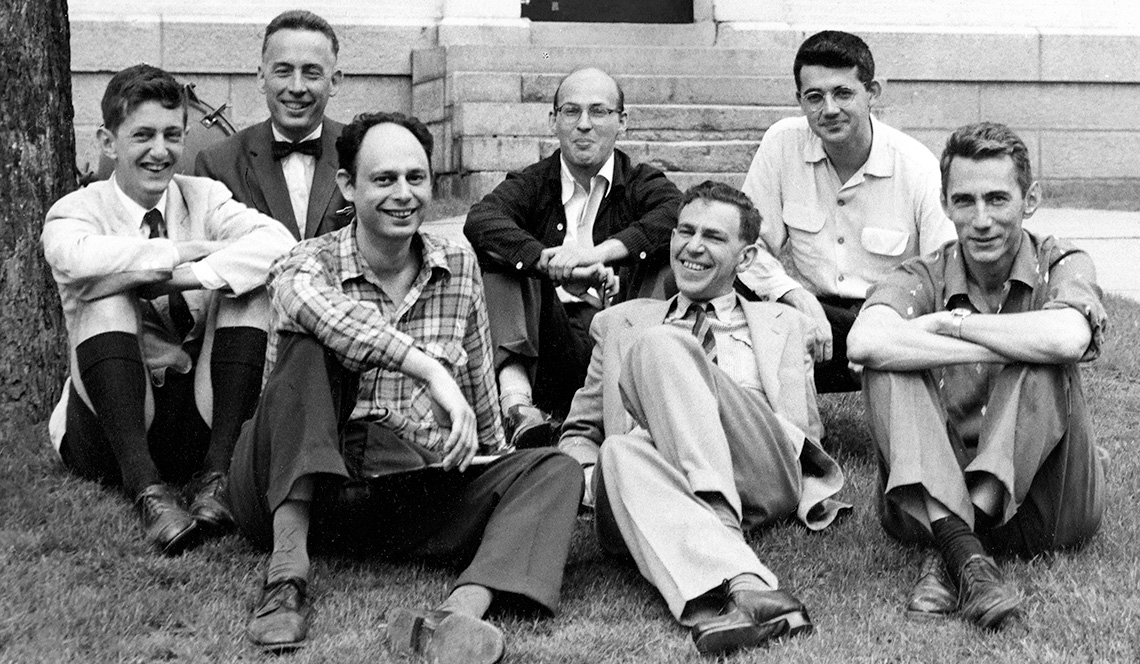
\includegraphics[width=0.5\textwidth]{images/Dartmouth-1956-Conference.jpg}
        \caption{达特茅斯会议}
    \end{figure}
\end{frame}

\subsection{1960s-70s: 符号 AI 与第一次 AI 寒冬}

\begin{frame}[t]{1960s-70s: 符号 AI 及其局限}
\begin{itemize}
    \item \textbf{符号 AI (GOFAI)}：专注于操作符号和逻辑规则来表示知识并解决问题。
    \item \textbf{ELIZA} (1966)：一个早期的自然语言处理程序，模拟罗杰斯心理治疗师。
    \item 符号 AI 在处理现实世界的复杂性和歧义时遇到困难。它需要大规模的手动编码知识库。
    \item \textbf{Lighthill 报告 (1973)}：批评 AI 未能实现其宏伟承诺，导致资金大幅削减 - \alert{第一次 AI 寒冬}。
\end{itemize}
\begin{figure}
    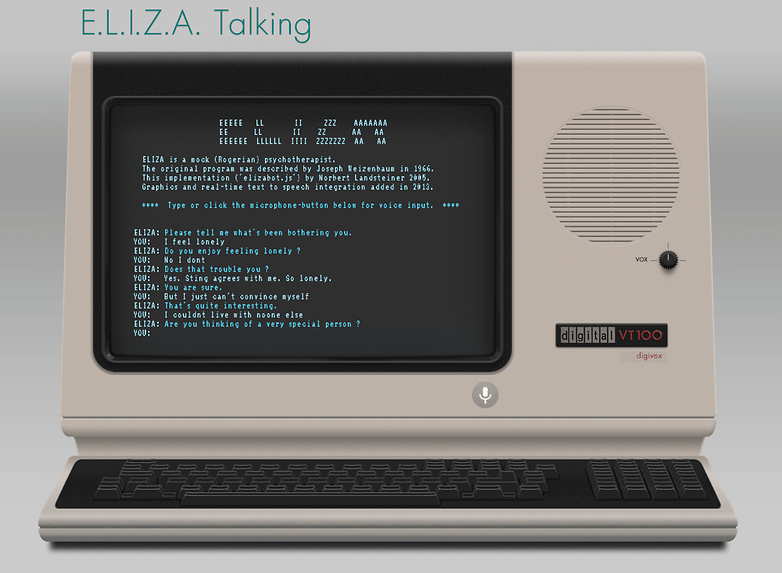
\includegraphics[width=0.4\textwidth]{images/eliza.png}
    \caption{ELIZA 程序}
\end{figure}
\end{frame}

\begin{frame}[t]
    \frametitle{LLAMA3.2 拜访 Emacs Doctor}
    \begin{figure}
    \begin{center}
        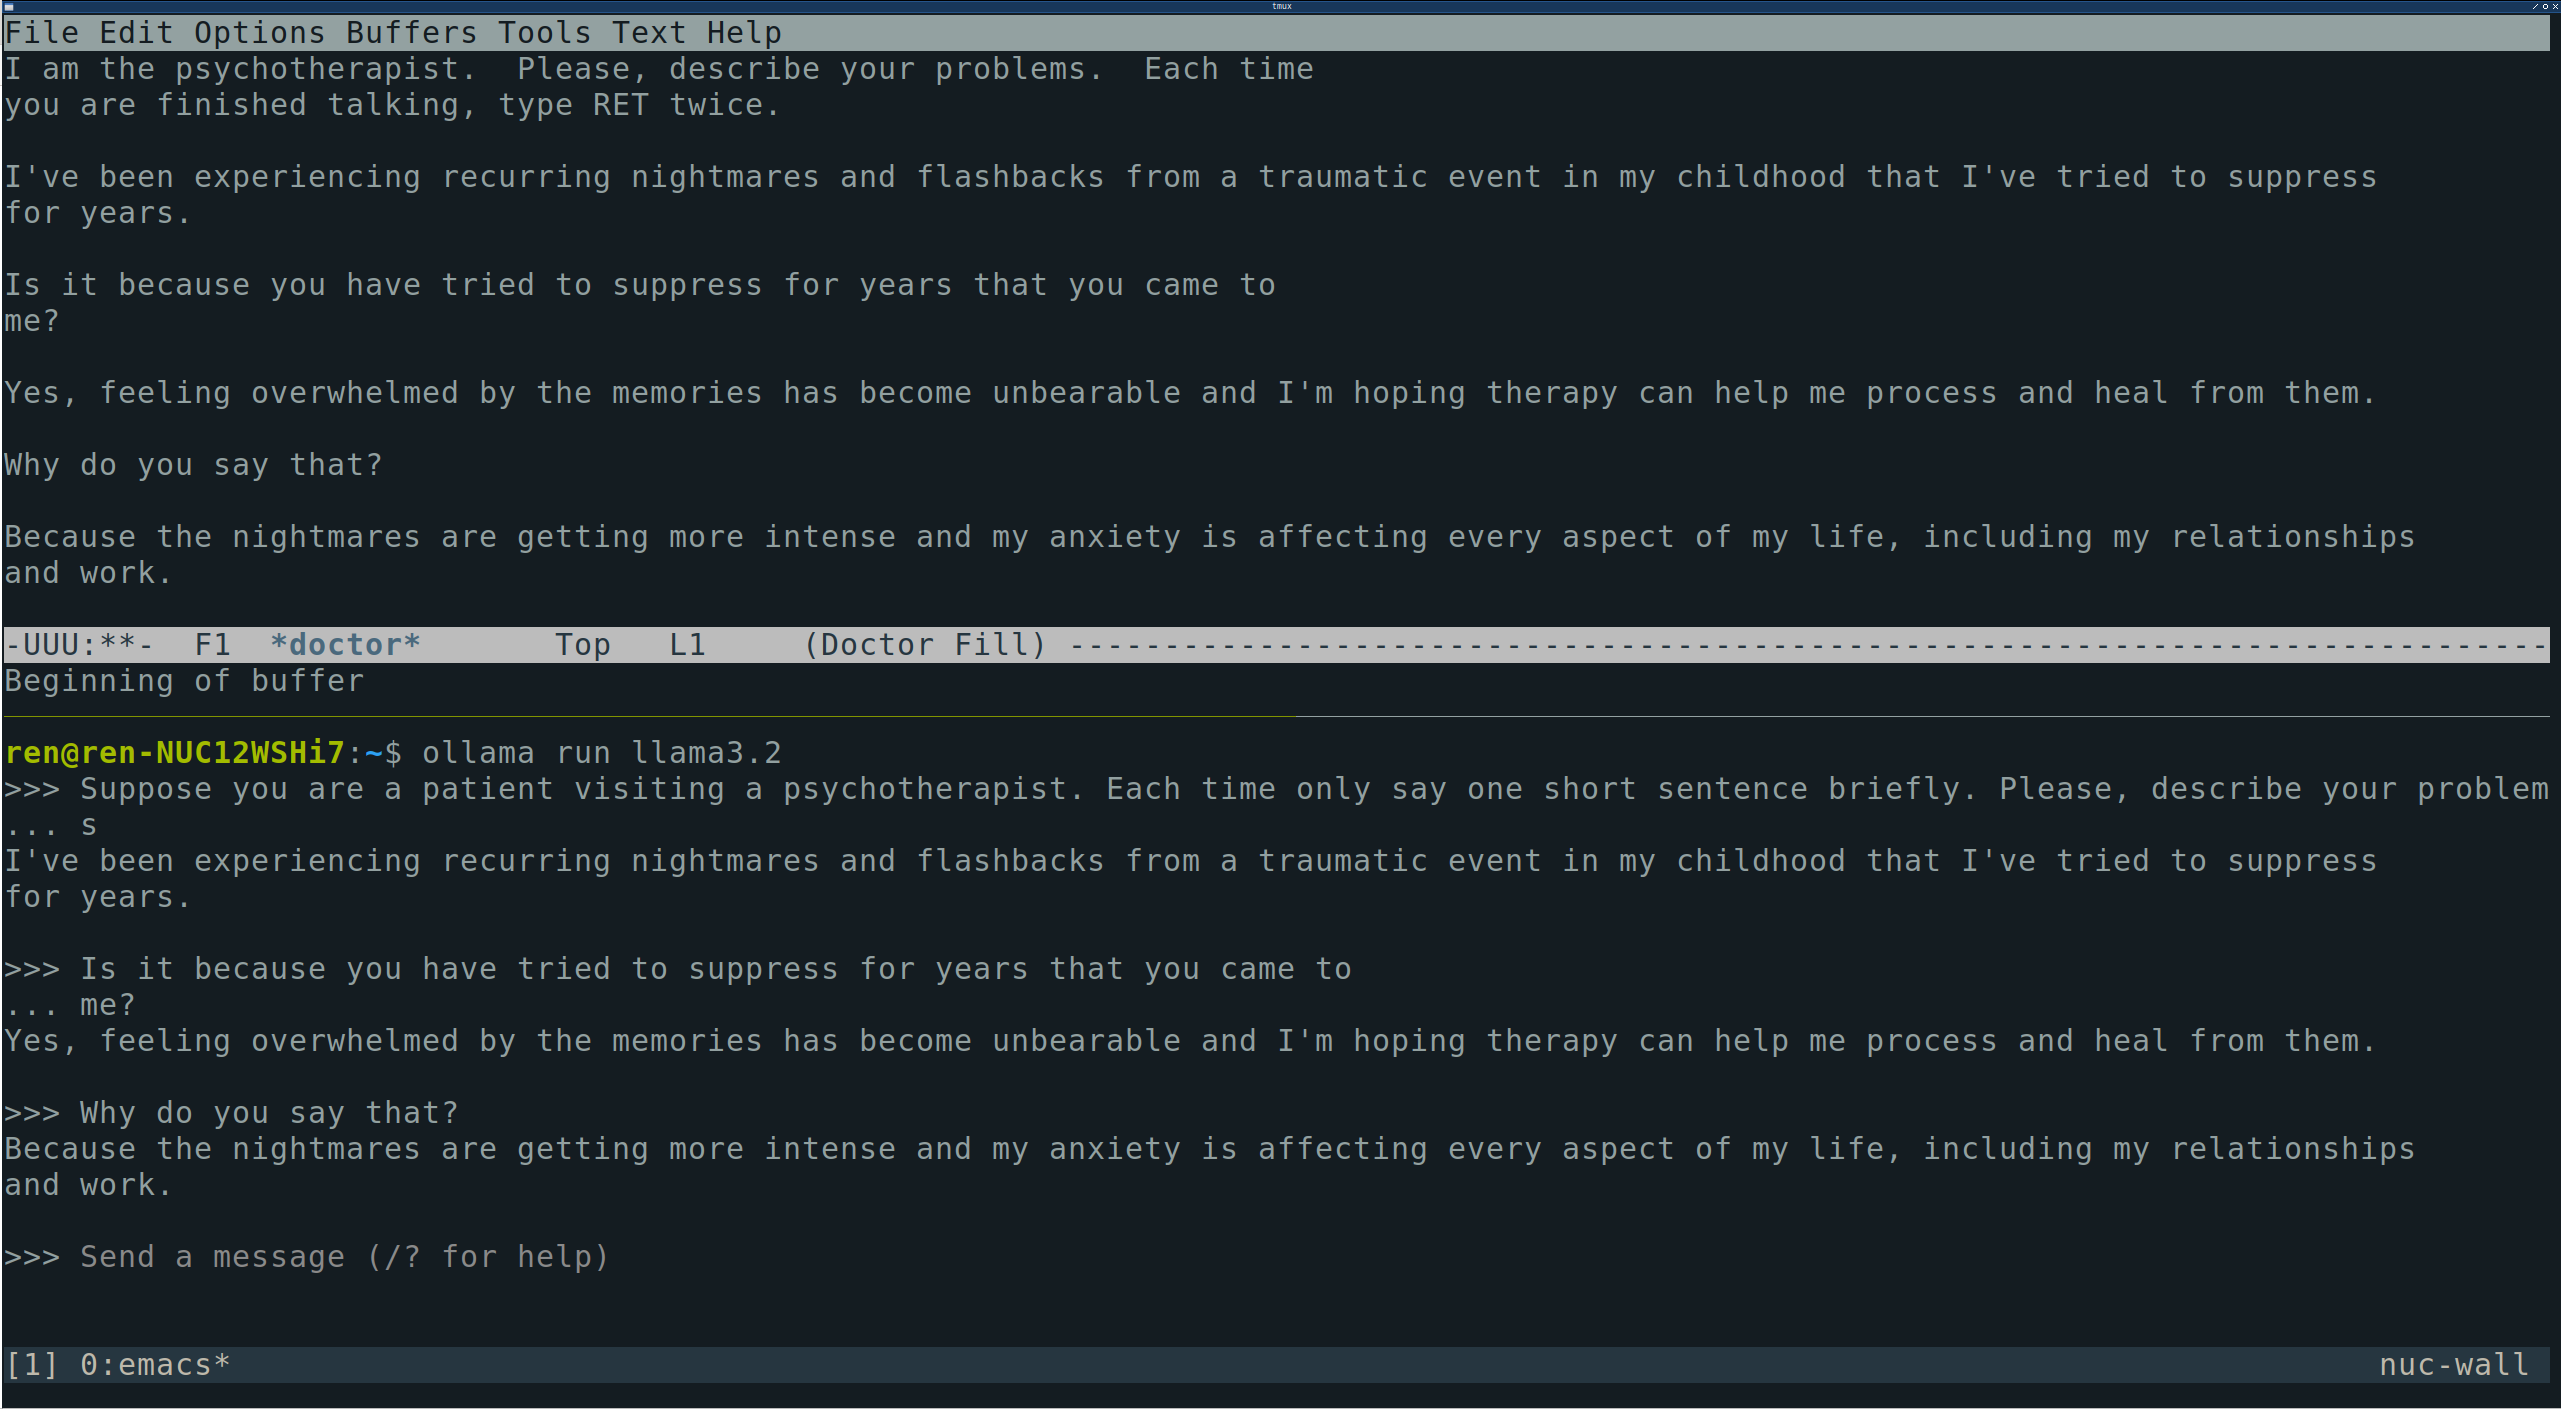
\includegraphics[width=0.9\textwidth]{images/doctor-llama.png}
    \end{center}
    \caption{LLAMA3.2 拜访 Emacs Doctor}
    \end{figure}
\end{frame}

\subsection{1980s: 专家系统与第二次 AI 寒冬}

\begin{frame}[t]{1980s: 专家系统的兴衰}
\begin{columns}
    \begin{column}{0.6\textwidth}
        \textbf{专家系统}
        \begin{itemize}
          \item 旨在通过基于规则的系统捕获人类专家的知识。
          \item 用于诊断血液感染的 MYCIN 系统表现与专家相当。
        \end{itemize}
        \textbf{第二次 AI 寒冬}
        \begin{itemize}
            \item 专家系统非常 \alert{脆弱}，维护成本高，且不具备学习能力。
            \item 它们无法扩展到狭窄领域之外。
            \item 到了1980年代末，炒作周期再次破裂，导致 \textbf{第二次 AI 寒冬}。
        \end{itemize}
    \end{column}
    \begin{column}{0.4\textwidth}
        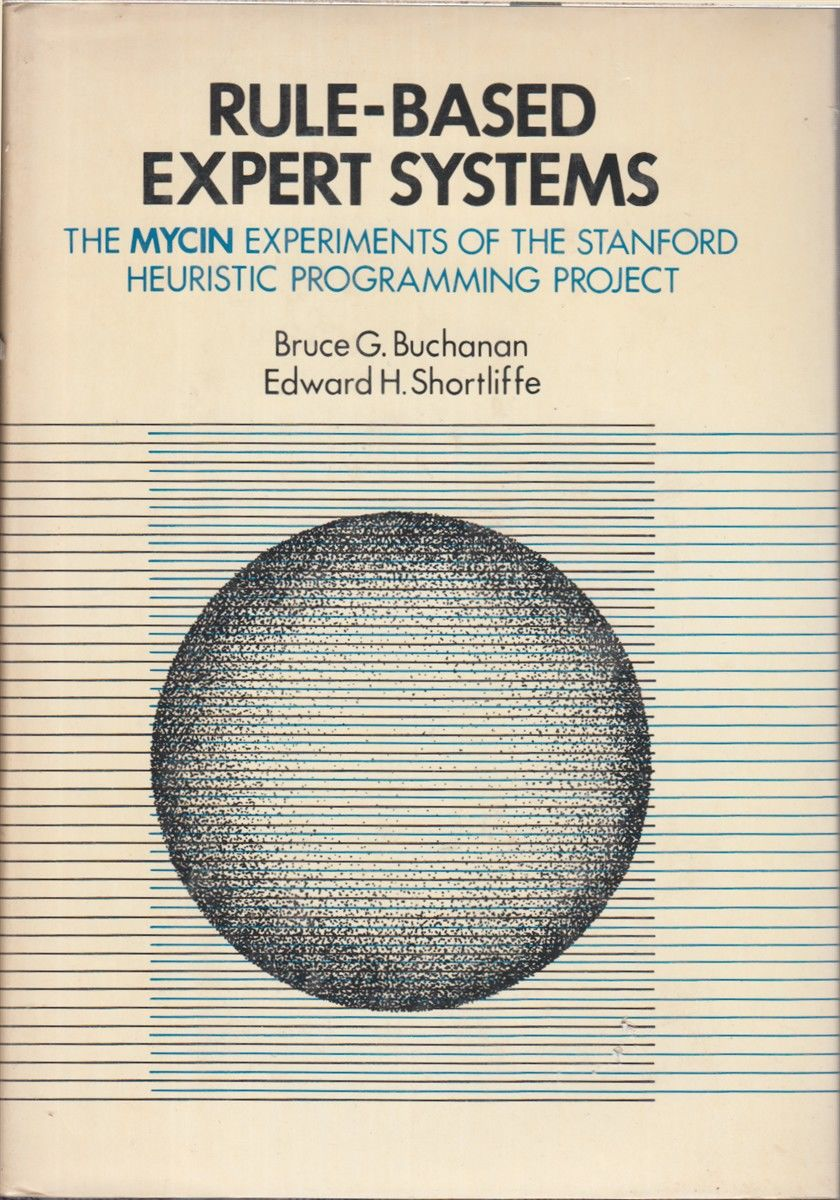
\includegraphics[width=0.9\textwidth]{images/mycin.jpg}
        \\\scriptsize{基于规则的专家系统}
    \end{column}
\end{columns}
\end{frame}

\subsection{1990s-2000s: 统计转型与机器学习}

\begin{frame}[t]{1990s-2000s: 新范式}
\begin{itemize}
    \item \textbf{从逻辑向统计的转变}：研究人员不再编程逻辑规则，而是专注于创建能够 \textbf{从数据中学习} 的系统（如 SVM、随机森林）。
    \item \textbf{IBM Deep Blue (1997)}：击败了世界象棋冠军加里·卡斯帕罗夫。这是符号 AI 的里程碑成就，主要依靠搜索和评估函数。
\end{itemize}
    \begin{figure}
        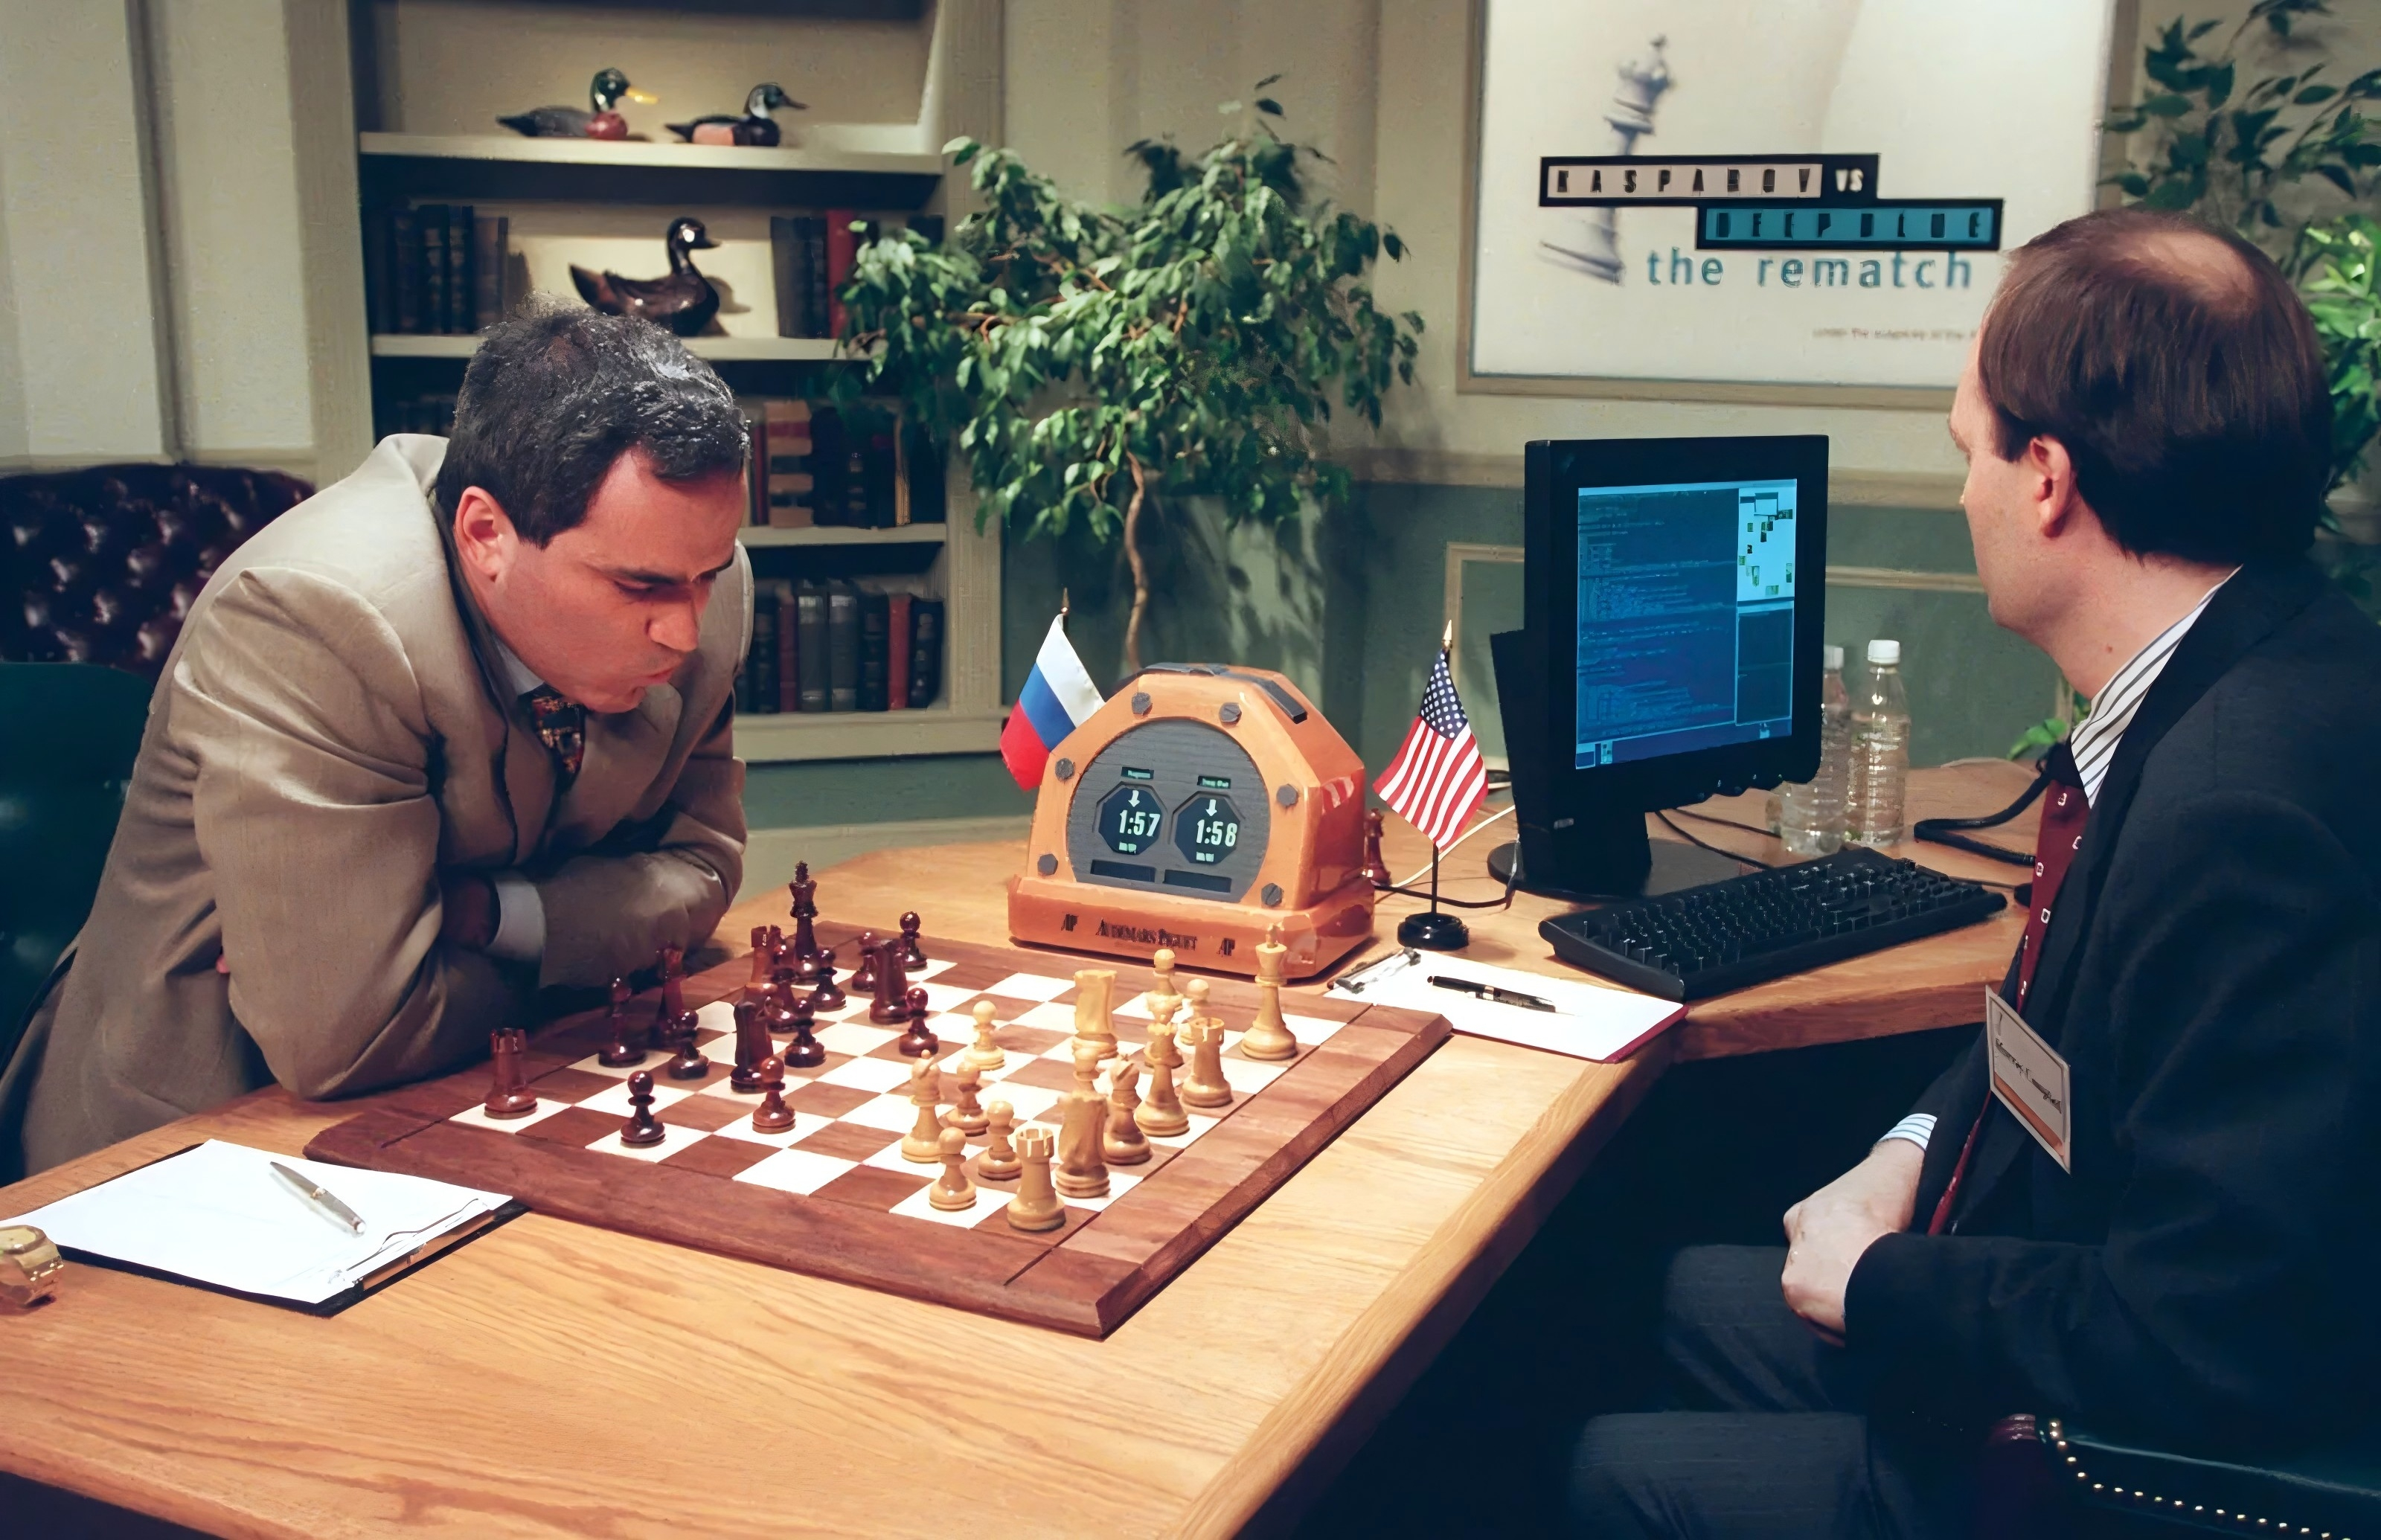
\includegraphics[width=0.5\textwidth]{images/Garry-Kasparov-Deep-Blue-IBM-computer.jpg}
        \caption{深蓝 vs. 加里·卡斯帕罗夫}
    \end{figure}
\end{frame}

\subsection{2010s: 深度学习革命}

\begin{frame}[t]{2010s: 深度学习爆发}
        \textbf{突破点}
        \begin{itemize}
            \item \textbf{关键促成因素}：海量数据集（大数据）和强大的并行计算能力（GPU）。
            \item \textbf{技术}：\textbf{深度学习} 使用多层神经网络，从原始数据中自动学习层次化特征。
        \end{itemize}
        \textbf{里程碑成就}
        \begin{itemize}
            \item \textbf{AlphaGo (2016)}：在围棋比赛中击败世界冠军，围棋曾被认为是人类智力游戏的最后堡垒。
        \end{itemize}
        \begin{figure}
            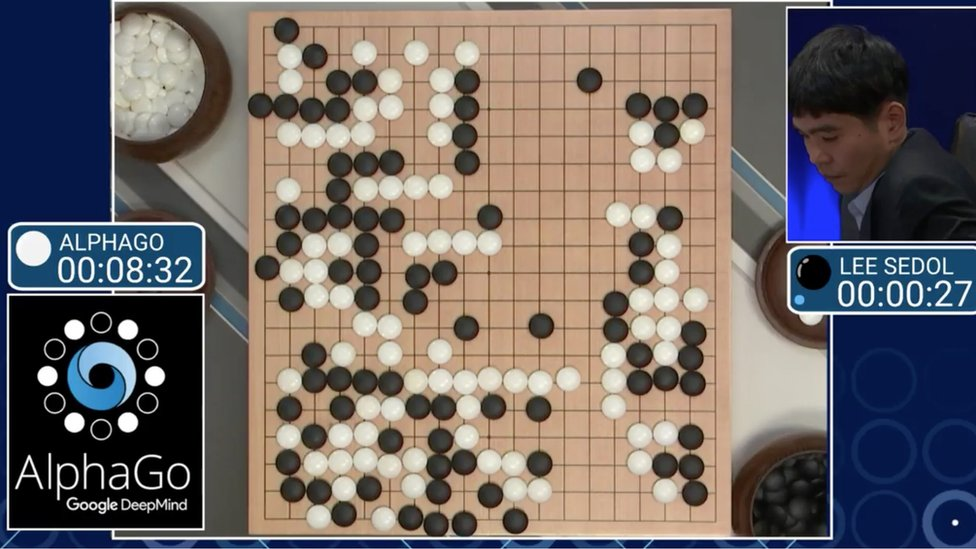
\includegraphics[width=0.4\textwidth]{images/alphago.jpg}
            \caption{AlphaGo vs. 李世石}
        \end{figure}
\end{frame}

\subsection{2020s: 大语言模型时代}

\begin{frame}[t]{2020s: LLM 与生成式 AI 时代}
\begin{itemize}
    \item \textbf{规模即一切}：发现大幅增加神经网络规模（大小、数据、计算量）会导致涌现能力的产生。
    \item \textbf{Transformer 架构 (2017)}：成为几乎所有现代 AI 的基础模型，实现了序列（如文本）的并行处理。
    \item \textbf{大语言模型 (LLMs)}：
        \begin{itemize}
            \item 像 GPT-4, Claude, Llama 这样的模型是在互联网大部分公开数据上训练的。
            \item 能够 \textbf{生成类人文本}、翻译、总结和编写代码。
        \end{itemize}
    \item \textbf{生成式 AI}：LLM 驱动了 ChatGPT 等工具，将 AI 能力带给大众。
    \item \textbf{多模态 AI}：能够理解和生成不同模态（文本、图像、音频）的模型。
\end{itemize}
\end{frame}

\subsection{结论}

\begin{frame}[t]{AI 历史：浪潮之旅}
\begin{center}
    \scriptsize{AI 领域经历了乐观的浪潮和随后的“寒冬”，每一次浪潮都在前人的基础上不断发展。}
\end{center}
\begin{block}{演进模式}
符号 AI (规则) $\rightarrow$ 统计机器学习 (数据) $\rightarrow$ 深度学习 (表示) $\rightarrow$ 生成式 AI (创作)
\end{block}
\end{frame}

\begin{frame}[t]{展望未来}
\begin{itemize}
    \item \textbf{通用人工智能 (AGI)}：人类水平智能的最初目标仍在远方。
    \item \textbf{伦理与安全}：随着 AI 变得强大，关于偏见、控制和与人类价值对齐的担忧变得至关重要。
    \item \textbf{AI 普及化}：AI 能力正在集成到几乎每一个软件产品中。
    \item \textbf{共生}：未来涉及人类与 AI 的紧密协作，增强人类的能力。
\end{itemize}
\begin{center}
    \textbf{制造思考机器的梦想比计算机本身更久远。这段旅程远未结束。}
\end{center}
\end{frame}

\section{跨学科结合课题}
\begin{frame}[t]{基于搜索的软件工程}
    基于搜索的软件工程 (SBSE) 将元启发式搜索技术（如遗传算法、模拟退火和禁忌搜索）应用于软件工程问题。软件工程中的许多活动都可以被表述为优化问题。由于计算复杂性或结构假设，运筹学的优化技术通常不适用于大规模软件工程问题。研究者使用对问题结构假设极少的元启发式搜索技术，来寻找近优解或“足够好”的解。
    \begin{figure}
    \begin{center}
        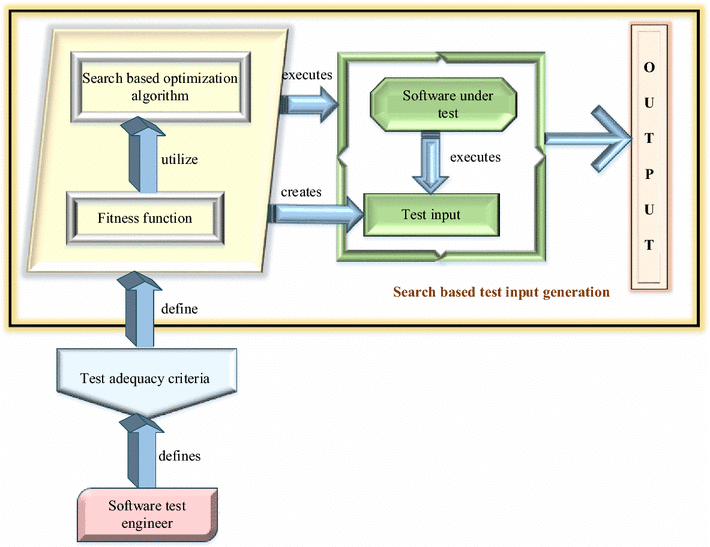
\includegraphics[width=0.5\textwidth]{images/Search-based-software-test-input-generation-method.png}
    \end{center}
    \caption{典型的 SBSE 工作流}
    \end{figure}
\end{frame}

\begin{frame}[t]{挖掘软件仓库}
在软件工程中，挖掘软件仓库 (MSR) 领域分析软件仓库中的丰富数据（如版本控制库、邮件列表归档、缺陷追踪系统等），以发现关于软件系统、项目和软件工程的有意义且可操作的信息。
    \begin{figure}
    \begin{center}
        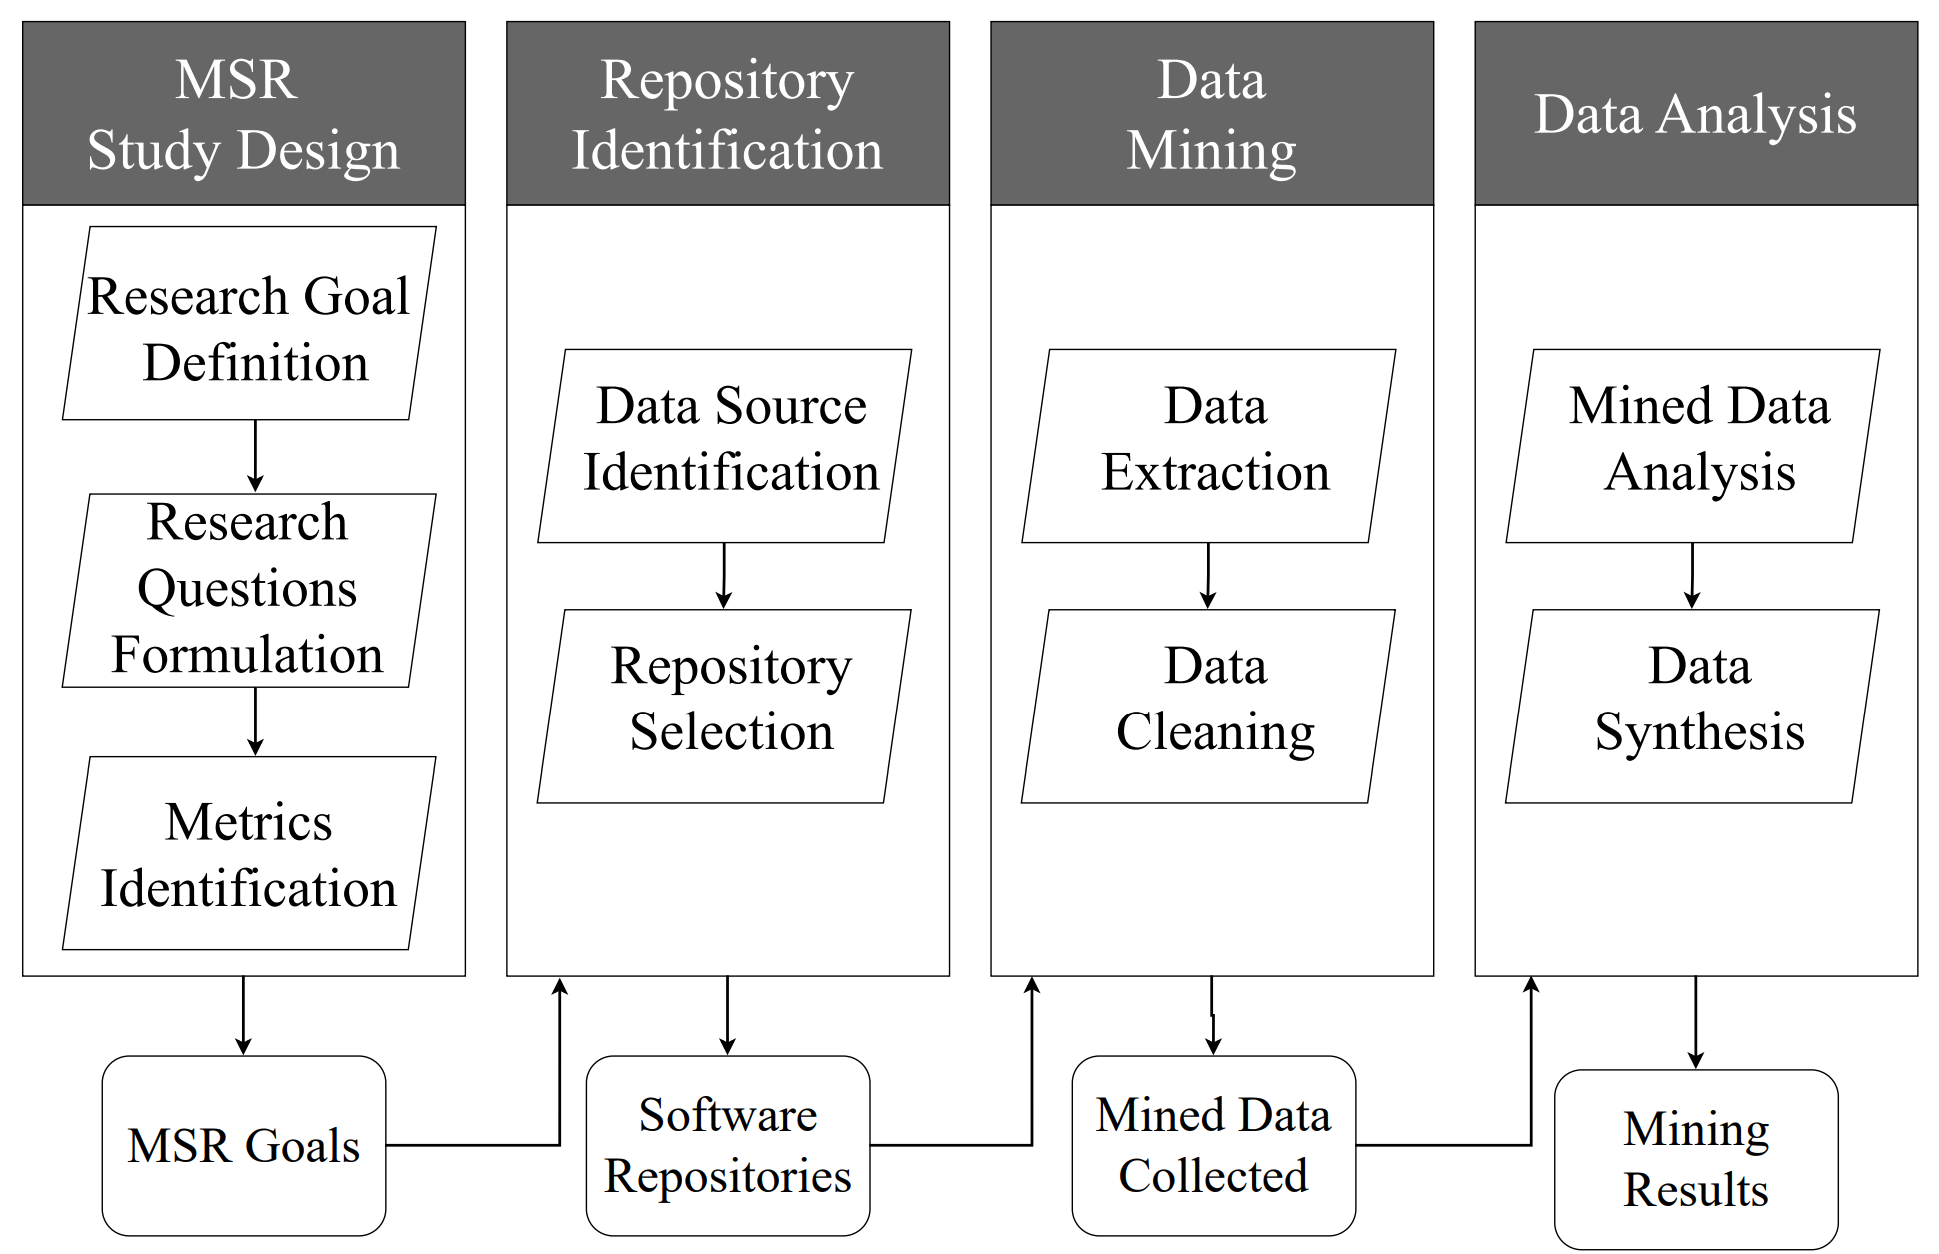
\includegraphics[width=0.5\textwidth]{images/msr.png}
    \end{center}
    \caption{典型的 MSR 工作流}
    \end{figure}
\end{frame}

\begin{frame}[t]{变更何时会引入修复？}
    \begin{figure}
        \subfloat[将事务链接到缺陷报告]{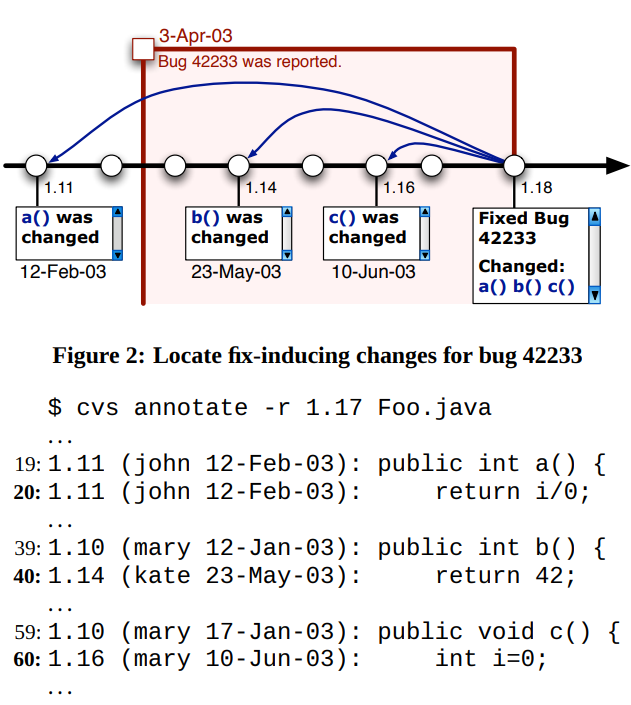
\includegraphics[height=4cm]{images/friday-1.png}}\qquad
        \subfloat[修复和修复诱导变更的分步]{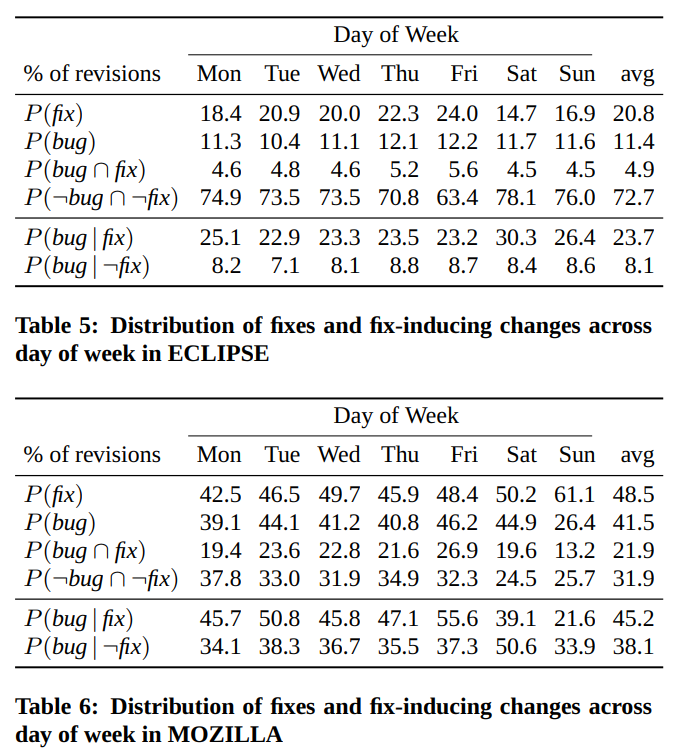
\includegraphics[height=4cm]{images/friday-2.png}}
        \caption{关于周五的研究}
    \end{figure}
\end{frame}

\begin{frame}[t]{为什么不要在周五写代码 (by Gemini)}
\begin{block}{理由 1：周末是神圣的}
\begin{itemize}
    \scriptsize
    \item \textbf{生产故障风险}：周五下午部署的 Bug 可能意味着整个周末都要进行紧急修复。
    \item \textbf{“多米诺效应”}：一个看似微小的问题可能连锁反应，需要多人协作解决。
    \item \textbf{压力与倦怠}：持续的周末加班是开发者职业倦怠的主要原因。
\end{itemize}
\end{block}

\begin{block}{理由 2：人为因素}
\begin{itemize}
    \scriptsize
    \item \textbf{人员可用性低}：关键人员（开发、测试、运维、支持）可能不在岗。
    \item \textbf{响应速度慢}：召集合适的团队解决问题需要更长时间。
    \item \textbf{周末疲劳}：周五的专注力自然下降，增加了出错的可能性。
\end{itemize}
\end{block}
\end{frame}

\begin{frame}[t]
\frametitle{主动方案：只读周五 (Read-Only Fridays)}
\begin{itemize}
    \item 将重心从部署新功能转向规划和准备。
    \item \textbf{活动包括}：
    \begin{itemize}
        \scriptsize
        \item 代码审查
        \item 编写文档
        \item 规划下周迭代
        \item 学习与专业发展
    \end{itemize}
    \item \textbf{目标}：在进入周末前保持生产环境的稳定和可预测性。
\end{itemize}
\end{frame}

\begin{frame}[t]{实证软件工程}
实证软件工程 (ESE) 是研究软件工程现象的子领域。该现象可以指软件开发工具、技术、实践、流程或组织因素。ESE 常用的研究方法包括：

\begin{enumerate}
    \item 初级研究（实验、案例研究、调查研究、模拟等）
    \item 次级研究（系统综述、系统映射研究等）
\end{enumerate}
\end{frame}

\begin{frame}[t]{UML 的实践现状}
    \begin{figure}
        \subfloat[声明的当前 UML 使用情况]{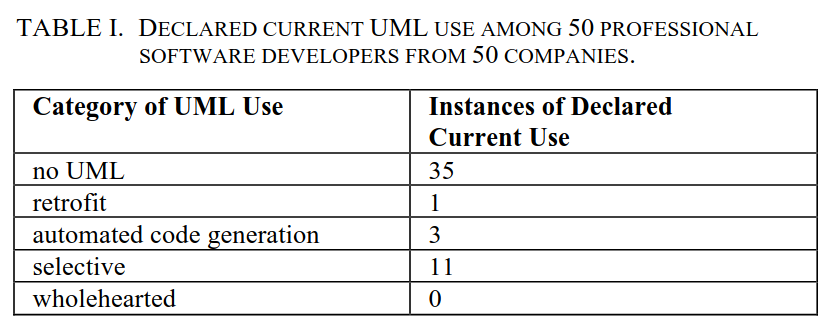
\includegraphics[height=2.2cm]{images/uml1.png}}\qquad
        \subfloat[11位“选择性”用户使用的 UML 图]{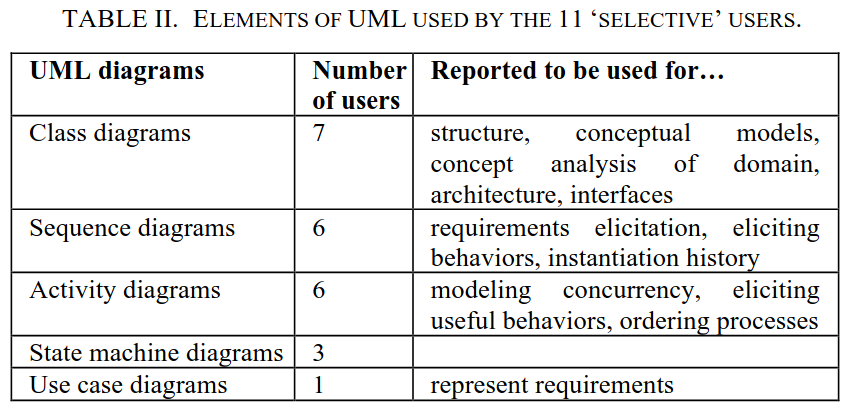
\includegraphics[height=2.2cm]{images/uml2.png}}
        \caption{UML 在实践中 (ICSE 2013)}
    \end{figure}
    \begin{block}{实践中的草图与图表 (FSE 2014)}
        \scriptsize
        大多数草图和图表是非正式的。40\% 根本不包含 UML 元素，48\% 包含部分元素，仅 9\% 完全由 UML 元素组成。受访者指出，即使使用了 UML，通常也没有严格遵守标准定义。
    \end{block}
\end{frame}

\begin{frame}[t]{参考文献}
\begin{thebibliography}{10}
\tiny
\bibitem{nato1968} NATO Software Engineering Conference (1968)
\bibitem{dijkstra1968} Dijkstra, E. W. (1968). Go To Statement Considered Harmful
\bibitem{brooks1975} Brooks, F. P. (1975). \textit{The Mythical Man-Month}. Addison-Wesley. 
\bibitem{thompson1984} Thompson, K. (1984). Reflections on Trusting Trust
\bibitem{stallman1983} Stallman, R. (1983). GNU Manifesto
\bibitem{beck2001} Beck, K. (2001). Agile Manifesto
\bibitem{llm2023} Chen, M. et al. (2023). Evaluating Large Language Models Trained on Code
\bibitem{fix} Śliwerski J, Zimmermann T, Zeller A. When do changes induce fixes?. 2005.
\bibitem{uml} Petre M. UML in practice. ICSE 2013.
\bibitem{sketch} Baltes S, Diehl S. Sketches and diagrams in practice. FSE 2014.
\end{thebibliography}
\end{frame}

\end{document}
